%%% The main file. It contains definitions of basic parameters and includes all other parts.

%% Settings for single-side (simplex) printing
% Margins: left 40mm, right 25mm, top and bottom 25mm
% (but beware, LaTeX adds 1in implicitly)
\documentclass[12pt,a4paper]{report}
\setlength\textwidth{145mm}
\setlength\textheight{247mm}
\setlength\oddsidemargin{15mm}
\setlength\evensidemargin{15mm}
\setlength\topmargin{0mm}
\setlength\headsep{0mm}
\setlength\headheight{0mm}
%% \openright makes the following text appear on a right-hand page
\let\openright=\clearpage

%% Settings for two-sided (duplex) printing
%\documentclass[12pt,a4paper,twoside,openright]{report}
%\setlength\textwidth{145mm}
%\setlength\textheight{247mm}
%\setlength\oddsidemargin{14.2mm}
%\setlength\evensidemargin{0mm}
%\setlength\topmargin{0mm}
%\setlength\headsep{0mm}
%\setlength\headheight{0mm}
%\let\openright=\cleardoublepage

%% Character encoding: usually latin2, cp1250 or utf8:
\usepackage[utf8]{inputenc}

%% Further useful packages (included in most LaTeX distributions)
\usepackage{amsmath}        % extensions for typesetting of math
\usepackage{amsfonts}       % math fonts
\usepackage{amsthm}         % theorems, definitions, etc.
\usepackage{bbding}         % various symbols (squares, asterisks, scissors, ...)
\usepackage{bm}             % boldface symbols (\bm)
\usepackage{graphicx}       % embedding of pictures
\usepackage{fancyvrb}       % improved verbatim environment
\usepackage{natbib}         % citation style AUTHOR (YEAR), or AUTHOR [NUMBER]
\usepackage[nottoc]{tocbibind} % makes sure that bibliography and the lists
			    % of figures/tables are included in the table
			    % of contents
\usepackage{dcolumn}        % improved alignment of table columns
\usepackage{booktabs}       % improved horizontal lines in tables
\usepackage{paralist}       % improved enumerate and itemize
\usepackage[usenames]{xcolor}  % typesetting in color
\usepackage{listings}
\usepackage{caption}
\usepackage{algorithm}
\usepackage[noend]{algpseudocode}
\usepackage{csquotes}
\usepackage{url}
\usepackage{blindtext}
\usepackage{enumitem}


%%% Basic information on the thesis

% Thesis title in English (exactly as in the formal assignment)
\def\ThesisTitle{Performance based adaptation of Scala programs}

% Author of the thesis
\def\ThesisAuthor{Petr Kubát}

% Year when the thesis is submitted
\def\YearSubmitted{2017}

% Name of the department or institute, where the work was officially assigned
% (according to the Organizational Structure of MFF UK in English,
% or a full name of a department outside MFF)
\def\Department{Department of Distributed and Dependable Systems}

% Is it a department (katedra), or an institute (ústav)?
\def\DeptType{Department}

% Thesis supervisor: name, surname and titles
\def\Supervisor{Tomáš Bureš}

% Supervisor's department (again according to Organizational structure of MFF)
\def\SupervisorsDepartment{Department of Distributed and Dependable Systems}

% Study programme and specialization
\def\StudyProgramme{Software Systems}
\def\StudyBranch{Software Engineering}

% An optional dedication: you can thank whomever you wish (your supervisor,
% consultant, a person who lent the software, etc.)
\def\Dedication{%
I would like to thank my supervisor, Doc. RNDr. Tomáš Bureš, PhD., for his help, valuable suggestions and ideas. I would also like to thank prof. Ing. Petr Tůma, Dr. for his consultations and advice. My thanks go to Mgr. Vojtěch Horký for setting up the environment to perform Spark tests. Last but not least, I would like to thank David Kuboň for providing useful feedback about the work.
}

% Abstract (recommended length around 80-200 words; this is not a copy of your thesis assignment!)
\def\Abstract{%
Dynamic adaptivity of computer system is its ability to modify the behavior according to an environment in which it is executed. It allows the system to achieve better performance, but usually requires specialized architecture and brings more complexity.

The thesis presents an analysis and design of a framework that allows simple and fluent performance-based adaptive development at the level of functions and methods. It closely examines the API requirements and possibilities of integrating such a framework into the Scala programming language using its advanced syntactical constructs. On theoretical level, it deals with the problem of selecting the most appropriate function to execute with given input based on measurements of previous executions.

In the provided framework implementation, the main stress is laid on modularity and extensibility, as many possible future extensions are outlined. The solution is evaluated on a variety of development scenarios, ranging from input adaptation of algorithms to environment adaptations of complex distributed computations in Apache Spark.
}

% 3 to 5 keywords (recommended), each enclosed in curly braces
\def\Keywords{%
{adaptive systems} {performance optimization} {run time prediction}
}

%% The hyperref package for clickable links in PDF and also for storing
%% metadata to PDF (including the table of contents).
\usepackage[pdftex,unicode]{hyperref}   % Must follow all other packages
\hypersetup{breaklinks=true}
\hypersetup{pdftitle={\ThesisTitle}}
\hypersetup{pdfauthor={\ThesisAuthor}}
\hypersetup{pdfkeywords=\Keywords}
\hypersetup{urlcolor=blue}

% Definitions of macros (see description inside)
%%% This file contains definitions of various useful macros and environments %%%
%%% Please add more macros here instead of cluttering other files with them. %%%

%%% Minor tweaks of style

% These macros employ a little dirty trick to convince LaTeX to typeset
% chapter headings sanely, without lots of empty space above them.
% Feel free to ignore.
\makeatletter
\def\@makechapterhead#1{
	{\parindent \z@ \raggedright \normalfont
		\Huge\bfseries \thechapter. #1
		\par\nobreak
		\vskip 20\p@
}}
\def\@makeschapterhead#1{
	{\parindent \z@ \raggedright \normalfont
		\Huge\bfseries #1
		\par\nobreak
		\vskip 20\p@
}}
\makeatother

% This macro defines a chapter, which is not numbered, but is included
% in the table of contents.
\def\chapwithtoc#1{
	\chapter*{#1}
	\addcontentsline{toc}{chapter}{#1}
}

% Draw black "slugs" whenever a line overflows, so that we can spot it easily.
\overfullrule=1mm

%%% Macros for definitions, theorems, claims, examples, ... (requires amsthm package)

\theoremstyle{plain}
\newtheorem{thm}{Theorem}
\newtheorem{lemma}[thm]{Lemma}
\newtheorem{claim}[thm]{Claim}

\theoremstyle{plain}
\newtheorem{defn}{Definition}

\theoremstyle{remark}
\newtheorem*{cor}{Corollary}
\newtheorem*{rem}{Remark}
\newtheorem*{example}{Example}

%%% An environment for proofs

%%% FIXME %%% \newenvironment{proof}{
%%% FIXME %%%   \par\medskip\noindent
%%% FIXME %%%   \textit{Proof}.
%%% FIXME %%% }{
%%% FIXME %%% \newline
%%% FIXME %%% \rightline{$\square$}  % or \SquareCastShadowBottomRight from bbding package
%%% FIXME %%% }

%%% An environment for typesetting of program code and input/output
%%% of programs. (Requires the fancyvrb package -- fancy verbatim.)

\DefineVerbatimEnvironment{code}{Verbatim}{fontsize=\small, frame=single}

%%% The field of all real and natural numbers
\newcommand{\R}{\mathbb{R}}
\newcommand{\N}{\mathbb{N}}

%%% Useful operators for statistics and probability
\DeclareMathOperator{\pr}{\textsf{P}}
\DeclareMathOperator{\E}{\textsf{E}\,}
\DeclareMathOperator{\var}{\textrm{var}}
\DeclareMathOperator{\sd}{\textrm{sd}}

%%% Transposition of a vector/matrix
\newcommand{\T}[1]{#1^\top}

%%% Various math goodies
\newcommand{\goto}{\rightarrow}
\newcommand{\gotop}{\stackrel{P}{\longrightarrow}}
\newcommand{\maon}[1]{o(n^{#1})}
\newcommand{\abs}[1]{\left|{#1}\right|}
\newcommand{\dint}{\int_0^\tau\!\!\int_0^\tau}
\newcommand{\isqr}[1]{\frac{1}{\sqrt{#1}}}

%%% Various table goodies
\newcommand{\pulrad}[1]{\raisebox{1.5ex}[0pt]{#1}}
\newcommand{\mc}[1]{\multicolumn{1}{c}{#1}}

\newcommand{\inlinecode}{\texttt}

\usepackage[linguistics]{forest}

% Settings of the code listings
\usepackage{listings}
\usepackage{color}
\usepackage[T1]{fontenc}
\usepackage[scaled]{beramono}

\usepackage{color}
%\definecolor{bluekeywords}{rgb}{0.13,0.13,1}
\definecolor{bluekeywords}{rgb}{0,0,0.5}
\definecolor{greencomments}{rgb}{0,0.5,0}
\definecolor{redstrings}{rgb}{0.9,0,0}
\definecolor{mygray}{rgb}{0.5,0.5,0.5}

\lstdefinestyle{Scala}{  
	language=Scala,
	showspaces=false,
	showtabs=false,
	breaklines=true,
	showstringspaces=false,
	breakatwhitespace=true,
	columns=fullflexible,
	escapeinside={(*@}{@*)},
	otherkeywords={},
	commentstyle=\color{greencomments},
	keywordstyle=\color{bluekeywords}\bfseries,
	stringstyle=\color{redstrings},
	basicstyle=\ttfamily,
	numbers=left,                    % where to put the line-numbers; possible values are (none, left, right)
	numbersep=12pt,                   % how far the line-numbers are from the code
	numberstyle=\color{mygray}, % the style that is used for the line-numbers
	rulecolor=\color{black},         % if not set, the frame-color may be changed on line-breaks within not-black text (e.g. comments (green here))
	stepnumber=1,                    % the step between two line-numbers. If it's 1, each line will be numbered
}

\lstdefinestyle{Dump}{  
	breakindent=0pt,
	breakatwhitespace,
	columns=fullflexible,
	showspaces=false,
	showtabs=false,
	breaklines=true,
	showstringspaces=false,
	breakatwhitespace=true,
	columns=fullflexible,
	escapeinside={(*@}{@*)},
	otherkeywords={},
	commentstyle=\color{greencomments},
	keywordstyle=\color{bluekeywords}\bfseries,
	stringstyle=\color{redstrings},
	basicstyle=\ttfamily,
	numbers=none,                    % where to put the line-numbers; possible values are (none, left, right)
	rulecolor=\color{black},         % if not set, the frame-color may be changed on line-breaks within not-black text (e.g. comments (green here))
}

\lstset{
%	language=Scala,
	showspaces=false,
	showtabs=false,
	breaklines=true,
	showstringspaces=false,
	breakatwhitespace=true,
	columns=fullflexible,
	escapeinside={(*@}{@*)},
	otherkeywords={},
	commentstyle=\color{greencomments},
	keywordstyle=\color{bluekeywords}\bfseries,
	stringstyle=\color{redstrings},
	basicstyle=\ttfamily,
	numbers=left,                    % where to put the line-numbers; possible values are (none, left, right)
	numbersep=12pt,                   % how far the line-numbers are from the code
	numberstyle=\color{mygray}, % the style that is used for the line-numbers
	rulecolor=\color{black},         % if not set, the frame-color may be changed on line-breaks within not-black text (e.g. comments (green here))
	stepnumber=1,                    % the step between two line-numbers. If it's 1, each line will be numbered
}

% Title page and various mandatory informational pages
\begin{document}
%%% Title page of the thesis and other mandatory pages

%%% Title page of the thesis

\pagestyle{empty}
\hypersetup{pageanchor=false}
\begin{center}

\centerline{\mbox{
\includegraphics[width=166mm]{./img/logo-en.pdf}}}

\vspace{-8mm}
\vfill

{\bf\Large MASTER THESIS}

\vfill

{\LARGE\ThesisAuthor}

\vspace{15mm}

{\LARGE\bfseries\ThesisTitle}

\vfill

\Department

\vfill

\begin{tabular}{rl}

Supervisor of the master thesis: & \Supervisor \\
\noalign{\vspace{2mm}}
Study programme: & \StudyProgramme \\
\noalign{\vspace{2mm}}
Study branch: & \StudyBranch \\
\end{tabular}

\vfill

% Zde doplňte rok
Prague \YearSubmitted

\end{center}

\newpage

%%% Here should be a bound sheet included -- a signed copy of the "master
%%% thesis assignment". This assignment is NOT a part of the electronic
%%% version of the thesis. DO NOT SCAN.

%%% A page with a solemn declaration to the master thesis

\openright
\hypersetup{pageanchor=true}
\pagestyle{plain}
\pagenumbering{roman}
\vglue 0pt plus 1fill

\noindent
I declare that I carried out this master thesis independently, and only with the cited
sources, literature and other professional sources.

\medskip\noindent
I understand that my work relates to the rights and obligations under the Act No.~121/2000 Sb.,
the Copyright Act, as amended, in particular the fact that the Charles
University has the right to conclude a license agreement on the use of this
work as a school work pursuant to Section 60 subsection 1 of the Copyright Act.

\vspace{10mm}

\hbox{\hbox to 0.5\hsize{%
In ........ date ............	% FIXME!
\hss}\hbox to 0.5\hsize{%
signature of the author
\hss}}

\vspace{20mm}
\newpage

%%% Mandatory information page of the thesis

\openright

\vbox to 0.5\vsize{
\setlength\parindent{0mm}
\setlength\parskip{5mm}

Title:
\ThesisTitle

Author:
\ThesisAuthor

\DeptType:
\Department

Supervisor:
\Supervisor, \SupervisorsDepartment

Abstract:
\Abstract

Keywords:
\Keywords

\vss}

\newpage

%%% Dedication

\openright

\noindent
\Dedication

\newpage

\openright
\pagestyle{plain}
\pagenumbering{arabic}
\setcounter{page}{1}


%%% A page with automatically generated table of contents of the master thesis

\tableofcontents

%%% Each chapter is kept in a separate file
\chapter*{Introduction}
\addcontentsline{toc}{chapter}{Introduction}

In modern software engineering, performance awareness has become a first class concern, as the systems deal with growing amounts of data, with higher emphasis on the real-time processing with more limited environments for embedded solutions and in general, as the requirements demand faster software while we are reaching the hardware limitations. It is the responsibility of the developer to assure that his code will not only work correctly, but also will be optimized and fast enough to meet these expectations.

The actual performance-aware programming can often be difficult and problematic for the developer, who is forced to make an assumptions about the speed of his program. The performance in general is, however, a dynamic, not a static feature. Even though it is possible to analyze the algorithm complexity at the design-time, the result will always be only an approximation, as it works with abstract elementary computational steps. In reality, the programs often behave in a different way due to the influence of CPU cache, memory locality, I/O operations, parallelism and many other factors. 

The only way how to actually find out if given implementation is fast enough, possibly faster than some other variant, is through a thorough testing process covering all the possible inputs and executed in the actual production environment. This process is complicated, costly, and should be repeated after every change in the program code, as it can have a previously unexpected impact. It can be partially automatized by introducing performance constraints to the classic unit tests, and there is an active research in this area, e.g. \cite{bulej_capturing_2012,horky_performance_2013,horky_utilizing_2015}.

Considering a common case where a programmer needs to decide which variant of implementation of some functionality to use, the discussed solution has some major downsides. First, he needs to design the tests, select the test data, execute them and make the decisions based on the results, which is a non-negligible effort, especially in a common software engineering process. Second, the decision made is final - once executed, the program will always have to use only the one, selected implementation. There are many cases where the performance of the implementations varies for different inputs or in different environments, and we would like our application to always use the best possible implementation, in other words, to adapt its execution to these conditions.

To address these problems and to simplify the performance-aware development in general, we propose a completely new approach in development, where the programmer identifies the implementation variants of a function in the code using a programming language construct. At execution, the system tracks the performance of the implementations involved and makes a new decision for each run of the function based on the inputs and current trends in the run times.

The goal of this thesis is to design a framework that would allow this way of development, to implement a prototype, to test it in various scenarios common for many applications where the approach might be beneficial, and to evaluate the actual advantages and problems of the proposed solution. The target platform of both the design and the implementation is the Scala programming language (\cite{noauthor_scala_nodate}), as it has a very flexible syntax suitable for creating language-like constructs, while being a statically typed language with both object oriented and functional foundations. In addition, many frameworks for data processing and similar tasks where the adaptation could be employed are either implemented or have interfaces in Scala, mainly for its high expressive powers. An example can be the Spark framework \cite{noauthor_apache_nodate}, which will be used in the evaluation process.

\subsubsection{Structure of the text}

In the first chapter of this work, the Scala language features that are not common among current object-oriented programming languages are introduced. Most of them will be mentioned and used in further chapters, so it serves as a brief introduction for a reader that knows basic OOP and functional languages, but does not have a deep knowledge of advanced Scala features.

The second chapter serves as a brief overview of the framework developed as a part of this thesis. More detailed goals are presented and a basic structure of the solution is outlined.

The third chapter is dedicated to the framework API. The reader is guided through the entire process of designing the API, from the requirement analysis and most simple use-cases, through possible drafts and their problems, the options that Scala offers, the actual design, its usage and problems, ending with more advanced scenarios and extensions. The whole chapter is written independently on the framework implementation, and is based only on the requirements and a basic notion of the functionality.

The fourth chapter is more theoretically focused. It introduces the functionality of the selection part of the framework on an abstract level. The whole process of deciding between multiple functions based on the historical observations of their runs is explained, and several algorithms are presented, tested and compared. In addition, more concrete improvements are suggested to increase the selection precision and to speed up the invocation process.

In the fifth chapter, the whole framework implementation is briefly presented. Concepts from the third and fourth chapters are incorporated into an actual Scala program. A couple of problems are mentioned and solved. Last but not least, the options that the framework user has of customizing and possibly extending the functionality are discussed.

The goal of the sixth chapter is to try out the framework in real-life scenarios and to evaluate the benefits that it brings. For that, a couple of different usage scenarios will be used, including basic selection between algorithms, JSON parsing or adapting to quickly changing network environment. A part of the chapter is devoted to the Spark framework for distributed data processing, which offers a great potential for adaptive execution.

In the last, seventh chapter, other work that is related to the problem of performance adaptation, measurement, prediction and similar topics is analyzed.
\chapter{Adaptation API design}

\section{The importance of API design}

API (Application Programming Interface) is a key component of every framework or library. It defines how a stand-alone piece of code (a function, class, module, or even entire running application) interacts with its environment. This includes the possible calls / requests, format of the data that is passed in as arguments and the data that is received as a result of the action.

APIs can be found on multiple levels of abstraction in a specific piece of software - % TODO 

.In our case, the API will be used to access functionality of our framework after adding our classes to the project.

\section{Basic API requirements}

The library itself should not require much interaction from the programmer. The usage would be based on performing some initial configuration, marking method implementations that are interchangeable, and then calling repeatedly either one of the methods marked, or some special method, and receiving correct results from one of the implementations.
In the optimal case, the library would be just added as a reference into the project and some minor changes would be done at the highest level, i.e. in the class method definitions, traits, adapters, etc. The business logic of the application should remain intact.
We can make a list of the \textbf{basic requirements}:
\begin{enumerate}
	\item Mark two or more methods as linked together (stating that they can be called interchangeably)
	\item Perform a call to the group of linked methods
	\item %TODO
\end{enumerate}

And some possible \textbf{extensions} to the API:
\begin{enumerate}
	\item Separate the selecting call and the evaluation call
	\item %TODO
\end{enumerate}

\section{Goals of the API design}

For a framework that will be used repeatedly by a variety of other developers, the API design is crucial and has several principal goals:

\begin{enumerate}
	\item Keeping the API calls simple in simple cases
	\item Giving the caller more options in more complicated cases
\end{enumerate}

\section{Advantages and disadvantages of Scala in API design}

% TODO: Macros

\section{Possibe API drafts}

\subsection{Direct interaction}

\subsection{Function composition}

Scala is a programming language that has absorbed a lot of concepts from the functional programming language world. Above all the key concept that functions are \textit{first-class values} and can be passed around the same way as code.

The goal of our API is to allow the programmer to link together two or more functions and receive one universal function that will decide which one to call. In a purely functional language, this could be solved using a \textit{higher-order function}\footnote{A function whose arguments and return type are other functions.}. It is a common approach

\lstset{language=Haskell}
\begin{lstlisting}
funA :: Ord a => [a] -> [a]
funB :: Ord a => [a] -> [a]

fun = selectFrom funA funB

fun :: Ord a => [a] -> [a]
\end{lstlisting}

\section{Scala API implementation}

%TODO: scala implicit casts

%TODO: scala function types (and nececity to duplicate code)

%TODO: extending function type, overriding apply()

%TODO: methods vs. functions in scala, eta expanstion

%TODO: multiple combination

%TODO: covariance and contravariance

\subsection{Covariance and contravariance}
So far, all mentioned usages of the \lstinline|or()| method were limited to functions with the same signatures. Quite common case, however, might be combining multiple functions with slightly different argument and return value types, typically one being a specialized version of the other. For example:

%TODO: replace this example:

The two functions can't be joined using the \lstinline|or()| method, because \lstinline|bubbleSort()| is defined on a more general type than \lstinline|radixSort()|. Let's examine simplified case with more combinations:

\lstset{language=Scala}
\begin{lstlisting}
def fun1(arg: Any): String = ???
def fun2(arg: String): Any = ???
def fun3(arg: String): String = ???

val fun4 = fun3 _ or fun2
val fun5 = fun2 _ or fun3
val fun6 = fun3 _ or fun1
val fun7 = fun1 _ or fun3
\end{lstlisting}

We receive compilation error on lines 5 and 8, in the definition of \lstinline|fun4| and \lstinline|fun7|. Lines 6 and 7 compile correctly. These are the cases where:

\begin{enumerate}
	\item Return type of the function passed in as an argument is a subtype of the return type of the target function
	\item Argument type of the function passed in as an argument is a supertype of the argument type of the target function
\end{enumerate}

The function types (represented as traits) in Scala are defined in the following way:
\lstset{language=Scala}
\begin{lstlisting}
trait Function1[-T1, +R] extends AnyRef
\end{lstlisting}

The type arguments representing the function arguments are defined as contravariant and the type argument representing the return value of the function is defined as covariant. This leads to \lstinline|(String) => String| being a subtype of \lstinline|(String) => Any| and to \lstinline|(Any) => String| being a subtype of \lstinline|(String) => String|. So the \lstinline|or()| method is working flawlessly for the \lstinline|fun5| and \lstinline|fun6|.

Taking into account that \lstinline|or()| is behaving like a commutative infix operator, we would like it to work in the other two cases as well. The two functions combined will always be in a subtype - supertype relation The signature of the function returned has to match the more limiting signature, i.e. the signature,

\begin{lstlisting}
def funA(arg: A): A = ???
def funB(arg: B): B = ???
val funAB: (B with A) => Object = funA _ or funB
\end{lstlisting}

%TODO: Comment case & listing

 As we can see, these are the cases where:

\begin{enumerate}
	\item The output type of the function that is passed as an argument is more general (superclass) than the output type of the target function
	\item The argument type of the function that is passed as an argument is more specific (subclass) than the argument type of the target function
\end{enumerate}

This is a case where covariance and contravariance of the type arguments of the functions that our \lstinline|or()| method accepts should be taken into account. Let's consider the following type of the first function:

\lstset{language=Scala}
\begin{lstlisting}
(A) => B
\end{lstlisting}

This function should be combinable using \lstinline|or()| method with any 

\subsection{Implicit arguments}

%TODO: How to solve this issue?

\lstset{language=Scala}
\begin{lstlisting}
def radixSort(list: List[Int]): List[Int] = ???
def bubbleSort[A <% Ordered[A]](list: List[A]): List[A] = ???
\end{lstlisting}

\lstset{language=Scala}
\begin{lstlisting}
def radixSort(list: List[Int]): List[Int] = ???
def bubbleSort[A](list: List[A])(implicit ord: A => Ordered[A]): List[A] = ???
\end{lstlisting}

%TODO: implementing traits using combined methods

%TODO: summary of the API approach, definition of key terms and points in adaptive lifecycle - method definition, function / closure creation (eta expansion), function combination, 

\section{Identifier selection}

The functions that we are going to select from have to be identifiable in the entire application. More specifically, we need to be able to store the runtime measurements for every function throughout the entire execution process. The functions might be referenced and called from various points in the library user's code. Additionally, we know nothing about the runtime state of the application memory at the point of entry into our function. So the auxiliary data have to be stored statically, in a special memory section dedicated exclusively to the framework, and the access has to be thread safe.

%TODO: Thread safety

The historical runtime measurements (run history) of a function can be identified using various approaches.

\subsection{Arbitrary identifiers}
User of the library could assign custom identifiers to the functions. Main advantage of this approach is the possibility to include description or documentation of the specific implementation in the identifiers. For example:

\begin{lstlisting}
quickSort
heapSort
\end{lstlisting}

\begin{lstlisting}
joinQuery
selectInQuery
\end{lstlisting}

Having meaningful identifiers leads to readable logs or measurement history dumps and to easier debugging in general. It, however, imposes new requirements on the user of the library and makes the API more complex. In addition, the identifiers would in almost all the cases exactly match the name of the function implementation.

\subsection{Randomly generated identifiers}
If we abandoned the idea of meaningfulness, we could assign automatically generated identifiers without the user having to specify them. Possible candidates could be sequential numbers or GUIDs. The identifiers would have to be created and matched with the function definitions or combi

%TODO: Evaluation, advantages, disadvantages, generation
\chapter{Solution overview}

This chapter will provide a basic overview of the solution presented and of the tasks that had to be solved in the process and that will be described with more details in later sections.

%TODO: Maybe add references to future chapters

\section{Detailed goals}
\label{sec:goals_revisited}

In the introduction, the basic goal of the thesis was mentioned in a very general manner - as a simple-to-use framework that allows the user to introduce variants into his program. Now, we will go a little deeper and present more detailed goals and the consequences they have for the implementation.

\subsubsection{A simple and fluent API}

We would like the programmer to be able to simply combine two or more functions or methods (in any combination), resulting into a new function that can be called again.

\lstset{style=Scala}
\begin{lstlisting}
def impl1(in: T): U = ???
def impl2(in: T): U = ???
val impl3: (T) => U = ???

val function = impl1 _ or impl2 or impl3
\end{lstlisting}

This means that we are going to have to work with implicit typecasts from function types and with eta-expansion.

\subsubsection{Transparent usage}

The function that was created by the combining process (in the rest of the text referred to as \textit{combined function}) should behave just like a normal function - the caller should not have to perform any special action and he should not be able to recognize that multiple implementations are involved.

\lstset{style=Scala}
\begin{lstlisting}
val result1: U = impl1(arg)
val result2: U = function(arg)
\end{lstlisting}

If the user, however, decides to combine the function that is already combined from $n$ simple functions one more time, the result should be a combination of $n+1$ functions, not a combination of $2$ functions where one of them is the original.

\lstset{style=Scala}
\begin{lstlisting}
val newFunction = function or impl4
\end{lstlisting}

Similar behavior can be achieved by introducing custom function trait implementations and reflecting it in the typecast.

\subsubsection{Measuring and storing run times}

Whenever the function is called and one of the implementations run, the run time (or other metric) has to be measured and stored. The storage should be statically accessible, because the function can be invoked from different contexts and we would like to share the history across the entire application. In order to identify the implementation in the static storage, we would need an identifier, preferably the name of the method (if a method is used). For that, we are going to have to use a compile-time macro.

\subsubsection{Selecting the most appropriate function in different cases}

As the key part of the library, we want to select the function to run each time. The selection should have 2 basic outcomes:

\begin{itemize}
	\item Select the function that is expected to have better performance on given input in current conditions if we are certain enough
	\item Select the function that we need to collect data for if we are not certain enough
\end{itemize}

The selection would be based on historical measurements of each function. We should be able to handle the following situations regarding the history data:

\begin{itemize}
	\item Functions whose run time does not depend significantly on the input - we expect that if one function has better performance than the other, it will not change with different input or environment
	\item Functions whose run time depends on some characteristics of the input (e.g. if the sequence is sorted)
	\item Functions whose run time is expected to be a function of the input size or some similar measurable feature of the input (e.g. length of the sequence to sort)
	\item Functions whose run time depends on the execution environment and is expected to change over time
\end{itemize}

This leads to a few requirements. Multiple selection strategies meeting the requirements of these cases will be necessary - we need to propose some decision making procedures that will reflect the certainty using the methods of statistical testing with given significance level. The user will have a way to customize the function combination in order to identify the case and configure the selection process correctly.

\subsubsection{Controlling the invocation behavior}

The invocation behavior should change in some situations - when we are sure enough that one option is better than the other in general, when we need to gather more data, when we need to save time and cannot perform the selection, or in other cases. Every combined function should have its state and some behavior plan, which would reflect some basic statistics and events on the functions.

We can achieve this by introducing a simple state machine logic and a language in form of a Scala DSL to create simple state machines.

\subsubsection{Possibility to extend the framework}

The framework should be modular, with its parts being easy to replace or extend. It should be possible for the user of the framework to incorporate his own implementations without having to change the framework code in any way, just by modifying the initial runtime construction.

The following extensions should be possible without changing the code of the framework, only by adding custom implementations:

\begin{itemize}
	\item Change the metrics that is measured for the functions
	\item Change the history storage
	\item Add, replace or extend the selection strategies
\end{itemize}

For this to work, the framework runtime will be created by composition with no close-coupling between modules. All of the runtime parts will communicate using trait interfaces. A simple form of IoC\footnote{Inversion of Control} configuration will be used for the composition.

\section{Key parts of the system}

Based on the extended goals presented in section \ref{sec:goals_revisited}, key parts of the solution can be identified and will be described in detail in the rest of the text.

\begin{itemize}
	\item \textbf{API and \inlinecode{CombinedFunction}} - a set of classes and methods that the user will be directly interacting with in order to and invoke the combined functions
	\item \textbf{Invocation policies} - a system of simple state machines to manage the invocation process with almost no overhead, handled directly in the \textit{CombinedFunction}
	\item \textbf{Selection strategies} - simple, stateless and isolated strategies that can decide about the most appropriate function to run given a historical measurements of all the functions
	\item \textbf{Function selector and invoker with the history storage} - module that will be responsible for selecting the method using a given strategy, invoking it, measuring the performance metrics and storing and retrieving the history data; it will be called by the \textit{CombinedFunction}
	\item \textbf{Configuration} - a static description of the function selector and invoker, can be changed by the user
\end{itemize}
\chapter{Adaptation API design and implementation}
\label{chapter:api}

\section{The importance of API design}

API (Application Programming Interface) is a key component of every framework or library. It defines how a stand-alone piece of code (a function, class, module, or even entire running application) interacts with its environment. This includes the possible calls / requests, format of the data that is passed in as arguments and the data that is received as a result of the action.

APIs can be found on multiple levels of abstraction in a specific piece of software - % TODO 

.In our case, the API will be used to access functionality of our framework after adding our classes to the project.

\section{Basic API requirements}

The library itself should not require much interaction from the programmer. The usage would be based on performing some initial configuration, marking method implementations that are interchangeable, and then calling repeatedly either one of the methods marked, or some special method, and receiving correct results from one of the implementations.
In the optimal case, the library would be just added as a reference into the project and some minor changes would be done at the highest level, i.e. in the class method definitions, traits, adapters, etc. The business logic of the application should remain intact.
We can make a list of the \textbf{basic requirements}:
\begin{enumerate}
	\item Mark two or more methods as linked together (stating that they can be called interchangeably)
	\item Perform a call to the group of linked methods
	\item %TODO
\end{enumerate}

And some possible \textbf{extensions} to the API:
\begin{enumerate}
	\item Separate the selecting call and the evaluation call
	\item %TODO
\end{enumerate}

\section{Goals of the API design}

For a framework that will be used repeatedly by a variety of other developers, the API design is crucial and has several principal goals:

\begin{enumerate}
	\item Keeping the API calls simple in simple cases
	\item Giving the caller more options in more complicated cases
\end{enumerate}

\section{Advantages and disadvantages of Scala in API design}

% TODO: Macros

\section{Possible API drafts}

\subsection{Method annotations}

\subsection{Untyped reflection interface}

\subsection{Direct interaction}

\subsection{Function composition}

Scala is a programming language that has absorbed a lot of concepts from the functional programming language world. Above all the key concept that functions are \textit{first-class values} and can be passed around the same way as code.

The goal of our API is to allow the programmer to link together two or more functions and receive one universal function that will decide which one to call. This could be solved using a \textit{higher-order function}\footnote{A function whose arguments and return type are other functions.}, which is a common approach in functional languages, well known from list manipulating patterns like \textit{map}, \textit{filter}, or \textit{fold}.

Scala supports this approach both in language features and in its standard libraries - as mentioned in \ref{subsec:metandfun}, functions are first class values and can be arguments of other methods or functions. A simple example could be function composition, which is implemented as a method on the function type traits (see \ref{subsec:functiontypes}):

\lstset{style=Scala}
\begin{lstlisting}
val timesTwo = (x: Int) => { x * 2 }
val plusOne = (x: Int) => { x + 1 }
val timesTwoPlusOne = timesTwo.andThen(plusOne)
\end{lstlisting}

We can achieve even more readable and natural looking code if we take advantage of the infix operator syntax (see \ref{subsec:infixops}):

\lstset{style=Scala}
\begin{lstlisting}
val timesTwoPlusOne = timesTwo andThen plusOne
\end{lstlisting}

Chaining of the methods / operators is possible as well:

\lstset{style=Scala}
\begin{lstlisting}
val manyOperations = timesTwo andThen plusOne andThen plusOne andThen timesTwo
\end{lstlisting}

Inspired by this readable and very simple syntax to compose functions which relies on only the basic syntactic features of Scala, we can try to design the API of the selection mechanism in the exactly same way:

\lstset{style=Scala}
\begin{lstlisting}
def or(fun: (T) => R): (T) => R = ???
...
val funAorB = funA or funB
\end{lstlisting}

\subsubsection{Advantages}
\subsubsection{Disadvantages}
\subsubsection{Consequences}

\section{Scala API implementation}

\subsection{Consequences of the choice}

The \lstinline|or()| method, in order to be used as an infix operator, has to be defined on the type that represents the first argument, in this case, a function. More specifically, any of the function types mentioned in \ref{subsec:functiontypes}. Because Scala doesn't support extension methods, we need to introduce a new type for functions containing this functionality, and an implicit conversion from the normal function type.

We need to cover all of the 23 original function type traits with custom type extensions, which will be mostly duplicated code - this reduces the maintainability and flexibility of the code. The trait files can be generated, but any change has to be reflected in the generating script first, before re-generating the code.

\subsection{Using the API with methods}
\label{subsec:apimethods}

Another thing to consider is that in most cases, the selection mechanism will be used with methods, not functions. As mentioned in \ref{subsec:etaexpansion}, Scala allows a simple conversion from methods to functions, which can be implicit in some cases. It would be preferable to omit the explicit conversions wherever it's possible.

We can try combining methods with Scala function composition:
\lstset{style=Scala}
\begin{lstlisting}
val composed = method1 andThen method2
\end{lstlisting}

This code won't compile with a suggestion to add the \lstinline|_| operator to \lstinline|method1| in order to treat it as a partially applied function (and to be able to call \lstinline|andThen()| method). Scala unfortunately doesn't perform implicit eta-expansion on the target of a method call. So after fixing the example, we get a fully working result:

\lstset{style=Scala}
\begin{lstlisting}
val composed = method1 _ andThen method2
\end{lstlisting}

On \lstinline|method2|, the eta-expansion is performed implicitly, because it's an argument of a method without overloads.

Now, in order to keep the same pattern working, we need to declare our \lstinline|or()| method in the following way:
\lstset{style=Scala}
\begin{lstlisting}
trait FunctionAdaptor[T, R] extends (T) => R {
  def or(fun: (T) => R): (T) => R = ???
}
\end{lstlisting}

If there is a suitable implicit conversion from \lstinline|(T) => R| to \lstinline|FunctionAdaptor[T,R]|, it is possible to use it in the same way as the \lstinline|andThen()| method:

\lstset{style=Scala}
\begin{lstlisting}
val fun = method1 _ or method2 or method3
\end{lstlisting}

Chaining in this case will not cause any problem, because the return value of the \lstinline|or()| method has the type of \lstinline|(T) => R| and can be combined again. It is, however, necessary to identify the case in the implementation and to handle it, otherwise, we would be building a tree of function pairs to choose from instead of choosing from all N values at once.

Note that changing or overloading the \lstinline|or()| method to accept directly \lstinline|FunctionAdaptor[T,R]| to handle the chaining case would break the syntax, as there would be implicit typecast (or even a function overload) blocking the implicit eta-expansion (see \ref{subsec:etaexpansion}). The following example demonstrates the result:

\lstset{style=Scala}
\begin{lstlisting}
def or(fun: FunctionAdaptor[T,R]): (T) => R = ???
...
val fun = method1 _ or method2 _  or method3
\end{lstlisting}

%TODO: Def macros?
%TODO: Move to a different section

\section{The API problems and their solution}

\subsection{Covariance and contravariance}
%TODO: Object-oriented polymorphism
% http://milessabin.com/blog/2012/04/27/shapeless-polymorphic-function-values-1/

So far, all mentioned usages of the \lstinline|or()| method were limited to functions with the same signatures. Quite common case, however, might be combining multiple functions with slightly different argument and return value types, typically one being a specialized version of the other. For example:

%TODO: replace this example:

The two functions can't be joined using the \lstinline|or()| method, because \lstinline|bubbleSort()| is defined on a more general type than \lstinline|radixSort()|. Let's examine simplified case with more combinations:

\lstset{style=Scala}
\begin{lstlisting}
def fun1(arg: Any): String = ???
def fun2(arg: String): Any = ???
def fun3(arg: String): String = ???

val fun4 = fun3 _ or fun2
val fun5 = fun2 _ or fun3
val fun6 = fun3 _ or fun1
val fun7 = fun1 _ or fun3
\end{lstlisting}

We receive compilation error on lines 5 and 8, in the definition of \lstinline|fun4| and \lstinline|fun7|. Lines 6 and 7 compile correctly. These are the cases where:

\begin{enumerate}
	\item Return type of the function passed in as an argument is a subtype of the return type of the target function
	\item Argument type of the function passed in as an argument is a supertype of the argument type of the target function
\end{enumerate}

The function types (represented as traits) in Scala are defined in the following way:
\lstset{style=Scala}
\begin{lstlisting}
trait Function1[-T1, +R] extends AnyRef
\end{lstlisting}

The type arguments representing the function arguments are defined as contravariant and the type argument representing the return value of the function is defined as covariant. This leads to \lstinline|(String) => String| being a subtype of \lstinline|(String) => Any| and to \lstinline|(Any) => String| being a subtype of \lstinline|(String) => String|. So the \lstinline|or()| method is working flawlessly for the \lstinline|fun5| and \lstinline|fun6|.

Taking into account that \lstinline|or()| is behaving like a commutative infix operator, we would like it to work in the other two cases as well. The two functions combined will always be in a subtype - supertype relation The signature of the function returned has to match the more limiting signature, i.e. the signature,

\begin{lstlisting}
def funA(arg: A): A = ???
def funB(arg: B): B = ???
val funAB: (B with A) => Object = funA _ or funB
\end{lstlisting}

%TODO: Comment case & listing

As we can see, these are the cases where:

\begin{enumerate}
	\item The output type of the function that is passed as an argument is more general (superclass) than the output type of the target function
	\item The argument type of the function that is passed as an argument is more specific (subclass) than the argument type of the target function
\end{enumerate}

This is a case where covariance and contravariance of the type arguments of the functions that our \lstinline|or()| method accepts should be taken into account. Let's consider the following type of the first function:

\lstset{style=Scala}
\begin{lstlisting}
(A) => B
\end{lstlisting}

This function should be combinable using \lstinline|or()| method with any 

\subsection{Generic methods}

%TODO: Solution suggestion - OOP approach, genericity in classes

%TODO: How to solve this issue?

Functions have one major limitation in Scala - they can't have any generic arguments. The signature of a function always has all the argument and return value types specified at compile-time. If we perform the eta-expansion on a generic method, we have to specify the type argument, otherwise, the type arguments will be fixed as Nothing and the function won't be callable:

\lstset{style=Scala}
\begin{lstlisting}
def makeTuple[A, B](a: A, b: B): (A, B) = (a, b)
val fun1 = makeTuple _
// fun1: (Nothing, Nothing) => (Nothing, Nothing)
val fun2 = makeTuple[Int, String] _
// fun2: (Int, String) => (Int, String)
\end{lstlisting}

As the \lstinline|or()| method performs combination of functions into another function, we automatically lose all the generic types involved in the original methods we are expanding and then combining. We can, however, take advantage of the fact that the type arguments being explicitly set in the process of eta-expansion can be generic types of an enclosing structure (generic class or generic method). With this approach, there are two possible patterns of achieving genericity in combined functions:

\begin{enumerate}
	\item Defining a function field inside a generic class
	\lstset{style=Scala}
	\begin{lstlisting}
	def defaultCount[A](list: List[A], item: A) = list.count(_ == item)
	def customCount[A](list: List[A], item: A) = list.filter(_ == item).map((i) => 1).sum
	
	class ListTools[A] {
	val count = defaultCount[A] _ or customCount[A]
	}
	\end{lstlisting}
	\item Defining a generic method by creating the combination and then calling it immediately
	\lstset{style=Scala}
	\begin{lstlisting}
	def count[A](list: List[A], item: A) = (defaultCount _ or customCount)(list, item)
	\end{lstlisting}
\end{enumerate}


Generics solution:
\lstset{style=Scala}
\begin{lstlisting}
def defaultMap[A, B](list: List[A], fun: (A) => B): List[B] = 
list.map(fun)
def iterativeMap[A, B](list: List[A], fun: (A) => B): List[B] =  {
val result = new mutable.MutableList[B]()
for (x <- list) {
result += fun(x)
}
result.toList
}

def map[A, B](list: List[A], fun: (A) => B): List[B] = 
(defaultMap[A, B] _ or iterativeMap[A, B])(list, fun)
\end{lstlisting}

\subsection{Implicit arguments}

Implicit arguments are arguments that will be filled in automatically at invocation by an implicit method with matching signature that is available within the scope. This can be used for different reasons, but the most common is a combination with a type argument that has to have a conversion of some kind. In the Scala terminology, the type has to be \textit{viewable} as some other type. There used to be a specialized syntax called \textit{View bounds} in earlier versions of Scala to support this usage, but it has been deprecated.

%TODO: http://docs.scala-lang.org/tutorials/tour/implicit-parameters.html

\lstset{style=Scala}
\begin{lstlisting}
def bubbleSort[A <% Ordered[A]](list: List[A]): List[A] = ???
def bubbleSort[A](list: List[A])(implicit ord: A => Ordered[A]): List[A] = ???
\end{lstlisting}

The most common usage of implicit arguments is simulating \textit{type classes} from other functional languages like Haskell. We create a generic trait with required methods (representing the type class and its functions) and whenever we want a new type to be member of the type class, we create implementation of the trait and an implicit method that provides the implementation. From now on, the newly added member can be used in any method requiring the implicit conversion just by importing our conversion function into the scope where the method is called.

%TODO: Example of custom "type class" or member?

As with a lot of other features, implicit arguments are supported only by methods, not by functions. Therefore, all of them have to be resolved and fixed when performing eta-expansion, along with all the type arguments. If we set the type arguments to a concrete type, we can provide the implementation in the same way as at the time of invocation, without any problem:

\lstset{style=Scala}
\begin{lstlisting}
def radixSort(list: List[Int]): List[Int] = ???
def bubbleSort[A <% Ordered[A]](list: List[A]): List[A] = ???

val sort = radixSort _ or bubbleSort[Int]
\end{lstlisting}

%TODO: Reference
There is, however, one more option mentioned in [REFERENCE] - the type argument can be set to a type argument of an enclosing scope, making the implicit argument generic again. In this case, the scope in which the type argument is declared has to provide the implicit function implementation. As a result, the implicit argument has to be repeated in the method or class constructor signature.

\lstset{style=Scala}
\begin{lstlisting}
def implicitFun1[A](list: List[A])(implicit ord: A => Ordered[A]): List[A] = ???
def implicitFun2[A](list: List[A])(implicit ord: A => Ordered[A]): List[A] = ???

// Following line won't compile:
// def implicitFun[A](list: List[A]): List[A] = (implicitFun1[A] _ or implicitFun2[A])(list)
def implicitFun[A](list: List[A])(implicit ord: A => Ordered[A]): List[A] = (implicitFun1[A] _ or implicitFun2[A])(list)d
\end{lstlisting}

\lstset{style=Scala}
\begin{lstlisting}
def bubbleSort[A](list: List[A])(implicit ord: A => Ordered[A]): List[A] = ???
\end{lstlisting}

\lstset{style=Scala}
\begin{lstlisting}
def implicitFun1[A <% Ordered[A]](list: List[A]): List[A] = ???
def implicitFun2[A <% Ordered[A]](list: List[A]): List[A] = ???

def fun = implicitFun1 _ or implicitFun2
\end{lstlisting}

Interesting thing is that the parser included in the IntelliJ IDEA IDE\footnote{Integrated Development Environment.} Scala plugin that performs background code inspection and immediately highlights compile-time errors doesn't recognize this problem. It was tested in version 2016.3.4 with Scala plugin version 2016.3.8.

%TODO: IntelliJ parser has no problems, compilation shows error

\lstset{style=Scala}
\begin{lstlisting}
def fun: (List[A]) => List[String] = implicitFun1 _ or implicitFun2
\end{lstlisting}

%TODO: Automatically generated type annotation is WRONG!!!

\subsection{Overloading}
Very similar issue is encountered when it comes to overloading - only methods can be overloaded.

%TODO: implementing traits using combined methods
\subsection{Implementing Traits}
Traits in the role of interfaces represent key element of object-oriented programming approach. Providing custom implementations of traits is essential and using adapted functions in this role would be very useful. The key problem is the separation of functions and methods in Scala mentioned in [REF].
%TODO: ADD REFERENCE HERE

The methods defined in traits can be implemented or overridden only by a different method, which will be invoked using virtual method calls. The function defined in the trait using a val keyword is basically a getter which returns the function value, invokable by itself. In this case, the getter has to be overridden, either by a custom getter, or by a field with automatically generated getter. An adapted function generated using the \lstinline|or()| method can be assigned to such a field and thus implementing the trait function getter. An example follows:

\lstset{style=Scala}
\begin{lstlisting}
trait TestTrait {
def testMethod(arg: List[Int]): List[String]
val testFunction: (List[Int]) => List[String]
}

class TestImpl extends TestTrait {
import functionadaptors.Implicits._

def impl1(arg: List[Int]): List[String] = 
arg.map("Num: " + _.toString)
def impl2(arg: List[Int]): List[String] = 
arg.map(i => s"Num: $i")

override val testFunction: (List[Int]) => List[String] = 
impl1 _ or impl2

// Can't implement testMethod using the result of or()
override def testMethod(arg: List[Int]): List[String] = ???
}
\end{lstlisting}

Unfortunately, a lot of the traits we need to provide implementations for are already existing and can use the method format. Manual workaround to implement the method is quite straightforward, but again, it generates unnecessary calls and duplicities in our code:

\lstset{style=Scala}
\begin{lstlisting}
...
private val adaptedFunction = impl1 _ or impl2
override def testMethod(arg: List[Int]): List[String] = 
adaptedFunction(arg)
...
\end{lstlisting}

%TODO: Add reference
Or, using the solution that was previously mentioned in [PREVIOUS SECTION], we can even omit the private field declaration and use an expression syntax:

\lstset{style=Scala}
\begin{lstlisting}
override def testMethod(arg: List[Int]): List[String] = 
(impl1 _ or impl2)(arg)
\end{lstlisting}


%TODO: summary of the API approach, definition of key terms and points in adaptive lifecycle - method definition, function / closure creation (eta expansion), function combination, 

%TODO: Thread safety

\section{Run history storage location}
\label{sec:storing}

The main concern of the selection mechanism design that is invisible to the user is all the data that will be gathered at runtime and used to select the appropriate variant. Assuming we have a function combined from two different implementations and it gets invoked at various points throughout the execution of the process, we have multiple options where to store the measurements.

All of the options were actually implemented and the API allows the user to chose storage location for every usage of the combiner.

\subsection{Local}

The first and most straightforward approach is to store all the measured runtime data inside the function object itself - we have a custom type \inlinecode{FunctionAdaptor} that is hidden to the user and that carries the references to function implementation, so it could hold the measurements for them as well.

The measurement data are specific for every instance of the adaptor and limited to it. This could have some use cases, for example classes that hold immutable data and provide some functionality that is based on the contained data, which is expected to be invoked repeatedly. The run history will then be specific for the data held by the instance and thus perfectly reflect performance in this one case.

There is a limitation connected to this use case - user of the API himself has to make sure that the adaptor instance will survive and be used in every call. Let's consider the following example:

\lstset{style=Scala}
\begin{lstlisting}
def processData(data: List[Int]): Int = 
  (impl1 _ or impl2 withStorage Storage.Local)(data)
\end{lstlisting}

In this case, during every invocation of the method \inlinecode{processData}, there will be new local instance of the \inlinecode{FunctionAdaptor} created by the \inlinecode{or} call. This instance will be used for the single call and then thrown away with the measured data. In order for this example to work properly, the adaptor has to be stored away:

\lstset{style=Scala}
\begin{lstlisting}
val impl = impl1 _ or impl2 withStorage Storage.Local
def processData(data: List[Int]): Int = impl(data)
\end{lstlisting}

\subsection{Global}

Another option is to store all the measured data globally, in a static area of the memory accessible from all contexts. A unique identifier has to be used to identify every one of the functions and methods combined.

The main advantage of this approach is that the run data are collected and stored from all invocation in the entire process, so there is more data to base the decision process on. This is usually the preferred approach for some business logic or utility methods in long-running services.

\subsection{Persistent}

The globally accessible runtime data can be 

This would be most useful (and probably the only means of using the ScalaAdaptive) for short-running tools with more variants of implementing the main logic. If the logic is invoked only once (or only a couple of times) during one invocation, there will never be enough data collected in a single run and it is necessary to persist the run history, saving data from multiple runs.

As the selection algorithms are delivering better results with growing data size, persisting the run history improves the selection mechanism in all the programs.

What can be a little problematic is deciding on when to persist the data. The logical solution to minimize the time spent on writing data is to store the entire run history once at the end of execution of the program. The runtime support, however, doesn't have any method of detecting when the program is about to end - JVM doesn't guarantee finalizers being called and relying on notifications from the user would complicate the API and generally be problematic.

The other approach is to update the persisted history with every run. Its downside is that the I/O operation might have negative impact on the performance if the function is called often and its run is fast. This impact can be limited by buffering the I/O - using the default Java I/O buffering mechanism would require leaving the file open for the entire application run, so custom buffer would be preferred. The buffer could be flushed upon every n-th write.

There are more problems connected with this solution, namely:
\begin{enumerate}
\item Running multiple instances of the application at once (collisions on the persisted data file) - especially if the file is left open
\item Changes in the application code (outdated run data, changed identifiers, etc.)
\item ...
\end{enumerate}
%TODO: More

\section{Run history storage identifiers}

In the globally accessible run history data storage, the data have to be assigned to a specific function. A unique identifier that would be derivable from the function objects passed into the \inlinecode{FunctionAdaptor} is required, so that whenever an adapted function is being executed, the runtime can access its history. 

In this case, references can't be used, because the \inlinecode{FunctionAdaptor} objects and the function objects wrapped inside can exist in multiple instances, can be deallocated and reallocated.

\subsection{Type name}

Functions in Scala are instances implementing the \inlinecode{FunctionN} trait. The default implementations are anonymous closure classes that are compiled from lambda expressions. Two different functions originated in two different lambda expressions and thus have two different type names, the ones that were generated and assigned by the compiler. The fully qualified type name can be used as the identifier of a function

Using the type names as unique identifiers is safe and straightforward. A small disadvantage is that they aren't very readable, the compiler uses the name of the type that contained the lambda expression followed by sequential number. 

There is also a subtle danger connected - in case of persisting the run history, the closure classes might get renamed automatically upon recompiling. The compiler usually assigns the closure names sequentially, so this could happen by just inserting another lambda expression into the enclosing class code before the current one. Run history data might even get mixed up as the newly added lambda expression could have the former name of the original closure (by taking its position in the sequence).

If the \inlinecode{FunctionN} trait has a different than default implementation, the type name identification might fail - the trait can be implemented by a single class wrapping other values. In this case, all functions implemented by that class would share the run history.

\subsection{Method name}
\label{subsec:methodnameident}

The most common usage pattern is the one where the functions used with the \inlinecode{or} method are eta-expanded methods (see \ref{subsec:apimethods}). The eta-expansion internally replaces the method name with a lambda expression wrapping the method call into a function. Consider the following example:

\lstset{style=Scala}
\begin{lstlisting}
def method(x: Int): Int = ???
def printName[T, R](fun: (T) => R) =
  println(fun.getClass.getTypeName)
...
printName(method)
\end{lstlisting}

Line 5 will print out \textit{Test\$\$anonfun\$main\$1}, a name of a closure class generated to encapsulate lambda expression. The closure itself gets compiled and so at runtime, there is no way of finding out, which method was called inside (i.e. which method it was expanded from).

If we, in case of eta-expanded methods, use the type name identifier, we run into a little problem - if a method is used in multiple \inlinecode{or} expressions, a different closure class is generated for each expression where it's eta-expanded. So in the following example, run history data of \inlinecode{method1} wouldn't be shared for runs originating from \inlinecode{combined1} and \inlinecode{combined2}:

\lstset{style=Scala}
\begin{lstlisting}
val combined1 = method1 _ or method2
val combined2 = method1 _ or method3
\end{lstlisting}

More convenient would be to use directly the names of the methods that are being eta-expanded. The names have to be extracted at compile time, using the def macros (see \ref{sec:defmacros}). At the moment of implicit conversion from \inlinecode{FunctionN} to \inlinecode{FunctionAdapterN}, the AST\footnote{Abstract syntax tree.} of the \inlinecode{FunctionN} expression can be examined - if it's a lambda expression containing one method call, the method name can be extracted.

Using method name identifier has some disadvantages as well. Firstly, all method overloads share the same identifier. Additionally, generic type arguments are not included in the identifier either.

\subsection{Custom identifier}

In order to handle the specific cases where type name and method name identifiers don't distinguish correctly between different functions, there is also a possibility of choosing a custom, arbitrary identifier. This has to be triggered specifically by the user in the API and should be used in the cases where:

\begin{enumerate}
	\item User knows that the automatically assigned identifiers won't be sufficient
	\item User wants to replace default type identifier with custom identifier because of readability
\end{enumerate}

%TODO: Evaluation, advantages, disadvantages, generation

\section{Extracting method name from eta-expansion AST}

In order to retrieve the method name to be used as an identifier (as explained in \ref{subsec:methodnameident}), we need to do the following:

\begin{enumerate}
	\item Replace the implicit conversion method from \inlinecode{FunctionN} to \inlinecode{FunctionAdaptorN} by a def macro (see \ref{sec:defmacros})
	\item Inside the macro, analyze the AST, detect eta-expansion method call
	\item If there is a method call:
	\begin{enumerate}
		\item Generate the identifier expression as a \inlinecode{getTypeName} call on the target of the method call, followed by the method name
		\item Generate the conversion code with explicitly specified reference expression
	\end{enumerate}
	\item Otherwise generate the conversion code with implicit reference	
\end{enumerate}

The conversion is done using the \inlinecode{toAdapter()} method with two overloads:
\begin{itemize}
	\item Accepting only the function - implicit reference is used (type name of the closure)
	\item Accepting the function and a custom reference - the reference provided is used
\end{itemize}

\subsection{Eta-expansion AST format}

First step in the macro implementation has to be parsing the input AST and detecting patterns that are generated from eta-expansions by the compiler. Using the \inlinecode{printAst()} macro mentioned in \ref{subsec:buildingast}, the following facts were discovered:

\begin{itemize}
	\item The eta-expansion is already replaced by the equivalent code in AST, so it can't be detected directly.
	\item The result of eta-expansion is a lambda expression (function literal).
\lstset{style=Dump}
\begin{lstlisting}
Function(...)
\end{lstlisting}
	\item The lambda expression is always wrapped in a block, being its return value.
	
\lstset{style=Dump}
\begin{lstlisting}
Block(
  List(...), 
  Function(...))
\end{lstlisting}	
	
	\item If the target of the invocation is either a constant or \textit{this}, it is captured in the lambda expression closure (i.e., the constant or \textit{this} is referenced directly from the function body).
	
	\item If the target of the invocation is a variable or a result of a more complicated expression, it is extracted to the enclosing block, its result is stored in a variable local to the block and then captured in the lambda expression closure. The reason is probably to avoid multiple evaluation of expressions with possible side-efects upon every invocation of the resulting function, and to avoid the target being changed throughout the lifetime of the function.
	
\lstset{style=Dump}
\begin{lstlisting}
Block(
  List(
    ValDef(
      Modifiers(SYNTHETIC), 
      TermName("eta$0$1"), 
      TypeTree(), 
      Apply(
        Select(
          This(
            TypeName("ClassName")), 
          TermName("getClassInstance")), 
        List()))), 
  Function(...))
\end{lstlisting}

	\item The function node contains argument definition and the expression itself, which is a single function application.

\lstset{style=Dump}
\begin{lstlisting}
Function(
  List(
    ValDef(
      Modifiers(PARAM | SYNTHETIC), 
      TermName("arg"), 
      TypeTree(), 
      EmptyTree)), 
  Apply(...))
\end{lstlisting}

	
%	\item The lambda expression (function literal) generated for the eta-expansion contains only the method invocation and the type applications (if the method is generic) - all the other expressions that are part of the eta-expansion are extracted to an outer, enclosing block, their results are stored in variables local to the block and then captured in the lambda expression closure. The reason is probably to avoid multiple evaluation of expressions with possible side-efects upon every invocation of the resulting function.
\end{itemize}

This has a few consequences for our case. We need to generate our conversion and method retrieval code into the block return value, because we need to be able to access the invocation targets that can be defined in the block itself. The target and the method name will always be in the single Apply node representing the function body.

If the method doesn't accept any type arguments, the tree is quite simple:

\lstset{style=Dump}
\begin{lstlisting}
Apply(
  Select(
    ...invocation target expression..., 
    TermName("methodName")), 
  List(...function arguments...))
\end{lstlisting}

Where the \textit{invocation target expression} can have multiple forms based on the original expression, and can depend on the enclosing block variables. It isn't, however, important for us, as we can work with the expression as whole. The function arguments are not needed either.

If the method is generic, the type arguments need to be applied in order to convert it to a function (which can't be generic). In this case, the tree gets a little more complicated:

\lstset{style=Dump}
\begin{lstlisting}
Apply(
  TypeApply(
    Select(
      ...invocation target expression..., 
      TermName("genericMethod")), 
    List(...type arguments...))), 
  List(...function arguments...))
\end{lstlisting}

The method call is wrapped in a TypeApply node before being invoked using the Apply node. The TypeApply node can in our case be ignored.

And the most complicated case we can encounter is when the method has some implicit arguments as well:

\lstset{style=Dump}
\begin{lstlisting}
Apply(
  Apply(
    TypeApply(
      Select(
        ...invocation target expression...,
        TermName("genericMethodImplicit")), 
      List(...type arguments...)), 
    List(...function arguments...)), 
  List(...implicit arguments...))
\end{lstlisting}

One more Apply node is added to the topmost level - the implicit arguments are applied after applying the actual function arguments. Their definition contains another nested block and lambda expression, but again, it is not necessary for our case. We just need to extract the invocation target and the method name.

\subsection{Generating the conversion}

Supposing we have the invocation target expression and the method name, we need to create the identifier string expression that will be used in the manual \inlinecode{toAdapter} invocation.

In order to extract the fully qualified name of the method call target, we need to generate the following expression:

\lstset{style=Scala}
\begin{lstlisting}
invocationTarget.getClass.getTypeName + ".methodName"
\end{lstlisting}

The AST representing this expression has to be wrapped in the \inlinecode{MethodNameReference} construction application (it is a case class with automatically generated \inlinecode{apply()} method) to get the resulting reference.

In all the cases, the \inlinecode{toAdapter} method has to be generated to replace the macro function. The function literal from the original AST has to be passed in as the first argument, and optionally, the second argument can be provided if the extraction of the method name was successful.

The original simplified tree looks like this:

\begin{forest}
	[Block
	  [Statements
	    [ValDef]
	  ]
	  [Function]
	]
\end{forest}

We need to transform the block, keeping the definition in the statement part, but wrapping the \inlinecode{Function} into the \inlinecode{toAdapter} call.
	
\begin{forest}
	[Block
	[Statements
	[ValDef]
	]
	[Apply
	  [toAdaptor]
	  [ArgumentList
	    [Function]
	    [ExtractedReferenceExpression]
	  ]
	]
	]
\end{forest}

\subsection{Extracting method overloads}

The approach that was described so far has one small issue - it doesn't recognize function overloads, so all the overloads share the same identifier.

 It wouldn't be difficult to extract the actual number of arguments that the method is being invoked with and include it in the reference. When attempting to extract the argument types of the lambda expression, we encounter a major problem - the function literal is generated without argument type specification, the TypeTree is empty:

\lstset{style=Dump}
\begin{lstlisting}
ValDef(
  Modifiers(PARAM | SYNTHETIC), 
  TermName("i"), 
  TypeTree(), 
  EmptyTree)
\end{lstlisting}

This can be done and is quite similar to the following piece of code:

\lstset{style=Scala}
\begin{lstlisting}
val function: (Int) => Int = { i => math.abs(i) + 1 }
\end{lstlisting}

In this case, the lambda expression doesn't have the type of its arguments specified either, because the compiler will infer it from the context in which the expression is used, in this case, from the type specifier of the variable.

The compiler is able to infer the data type from the usage of the argument as well:
\lstset{style=Scala}
\begin{lstlisting}
def method(i: Int): Int = ???
val function = { i => method(i) }
\end{lstlisting}

The previous piece of code is correctly compiled by the Scala compiler, although some IDEs (namely IntelliJ IDEA 2016.3.4) aren't able to infer the type and mark the code as incorrect.

Note that the eta-expansion is guided by the same rules, so whenever expanding a method without overloads, the compiler infers the types by itself:
\lstset{style=Scala}
\begin{lstlisting}
def method(i: Int): Int = ???
val function = method _
\end{lstlisting}

Upon expansion of a method with overloads, the resulting function type has to be provided and the inference flow goes in the other direction:
\lstset{style=Scala}
\begin{lstlisting}
def method(i: Int): Int = ???
def method(s: String): Int = ???
val function: (String) => Int = method _
\end{lstlisting}

As a consequence, at the time of syntax analysis, the types aren't inferred yet and there is no way for us to find out which method overload is being called.

The method overloads have to share the same identifier, but in most typical cases, this isn't a problem. Otherwise, it can be solved by using custom identifiers.
	
\section{Delayed measuring}

In some specific cases it might be useful to delay the measurement, or, in general, to measure invocation of a different function than the one that has multiple implementation. The implementations can affect something else than their own runtime. Some example use cases might be:

\begin{itemize}
	\item Configuration, or generation of configuration
	\item Expression tree building
	\item Query building
	\item Method chain building
\end{itemize}

It is obvious that our API, which was designed to remain as simple as possible, doesn't support this case. We need to slightly extend it.

\subsection{Decision context}

Supposing we already have a mechanism to mark the actual function to measure, we encounter another problem. Making a decision when executing the function with multiple implementation automatically generates a context of the decision - all measured function invocations that were affected by the decision. When measuring the invocation, the framework has to know to which context it belongs in order to be able to assign the measured data to the run history of the corresponding function.

The contexts can interleave and we can't match the decision with the invocation by time or location. It is impossible to decide to which decision which invocation belongs automatically - we need support from the framework user. The user will have to explicitly state the context whenever invoking the measured function. By doing this, he will pinpoint the moment of decision that affected the invocation.

Practically, we need to introduce a special object - the \textbf{measurement token} - which will represent the context. The \inlinecode{MultiFunction} instances will have a special, modified version of the apply method, which will not trigger the measure of the selected function, but will generate a measurement token, that will be used to measure future function runs.

\lstset{style=Scala}
\begin{lstlisting}
val getConfig = getFastConfig _ or getSlowConfig
val (config, measure) = getConfig^()
...
measure(() => run(config))
\end{lstlisting}

This approach has one main disadvantage compared to the rest of the API - it isn't transparent. The user has to know that he is working with the \inlinecode{MultiFunction}, not just normal function. His assistance is, however, required by the nature of the problem.

%TODO: Use cases - configuration generation, expression tree building, query building...

%TODO: Problems - matching decision with measurement
\chapter{Adaptive function selection}
\label{chap:deciding}

The key purpose of the adaptive framework is to always invoke a function that is expected to have the best performance possible in a given environment and with given inputs. By \textit{function performance} we mean any measurable description of the qualities of the function. It can be the actual run time of the function, memory consumption, number of I/O operations, number of threads created, execution counts for various parts of the code, etc. All these factors can be valuable and be the goal of the system run optimization.

This thesis is focused on the task of optimizing the function run time or time complexity in general. The core of the framework, however, is designed to be extensible by modules that can analyze the function run in different ways. More on this topic will be covered in chapter \ref{chap:implementation}.

Note we will suppose some basic knowledge of mathematical statistics in this chapter. A nice introduction covering all the concepts that this text works with can be found in \cite{weiss_introductory_2010}.

\section{Overview of the selection process}
\label{sec:selection_overview}

Suppose we have functions $f_1,\dots, f_n$, all of them interchangeable, and an input $in$\footnote{If the original Scala function has multiple arguments \inlinecode{arg1, ..., argN}, we will consider them to be a tuple \inlinecode{(arg1, ..., argN)} to get a single input object.}. We need to decide which of the functions to select and invoke. To be able to do that, we need to formulate predictions about run times of the functions under given circumstances, and then use the function with the lowest prediction. As the internal structure of the functions is unknown to us, the only data we can base the prediction on is the information we collect during previous executions of the individual functions. The exact form of these \textit{historical data} will be discussed later.

\subsection{Problems of the prediction and selection process}

There are three main factors we should take into account when predicting run times and using them to select a function:

\begin{itemize}
	\item The run times may depend on the input $in$
	\item The run times may depend on the environment
	\item The predictions are never precise, they have certain probability based on the amount and the character of the historical data
\end{itemize}

The \textit{input dependency} problem is being solved in many works about program execution time predictions. Certain features of the input are usually analyzed and a model is constructed describing the relation to the run time. The model can then be used to predict the times for new inputs. This approach was used in \cite{chun_mantis:_2010,goldsmith_measuring_2007}. The authors of \cite{smith_predicting_1998} propose clustering the inputs prior to creating any models.

The \textit{environment dependency} is more complicated - there are no factors that we could watch and use to classify the runs or to include in the prediction model. The simplest solution is to give the history records a limited duration after which they expire. The environment changes are not expected to occur very often, which makes the most recent data the most suitable for modeling and predicting. This technique is suggested among the adaptive framework use-cases in \cite{bulej_performance_2012}.

As for the \textit{uncertainty} problem, works in this field tend to use statistical methods to express the confidence of the prediction. In \cite{smith_predicting_1998}, confidence intervals are used for this purpose. The comparison of predictions used for selection should aways take these information into account and reject to select any function in case of uncertainty to prevent potentially wrong decision. Such a case should be solved by executing the function with the least data to gather more observations.

\subsection{Input in the prediction process}
\label{subsec:input_in_selection}

The input of the function can be a complex structure with multiple factors contributing to the run time\footnote{Consider for example a general graph - for most of the algorithms, both number of vertices and edges have to be taken into account}. Common prediction techniques (\cite{chun_mantis:_2010,goldsmith_measuring_2007}) use simplified model of the input $in$ represented by a vector of \textit{features} $(t_1, \dots, t_n)$. 

Based on this approach, we will suppose that for each Scala function exists $g$ so that for each input $in$ modeled by $(t_1, \dots, t_n)$ holds \(t = g(t_1, \dots, t_n) + \varepsilon\), where \(t\) is the runtime of the function on input \(in\), and $\varepsilon$ is an error represented by a random variable with certain distribution, which we, for simplicity, assume to be normal. 

Now, the \textit{features} can be divided into 2 basic categories:

\begin{itemize}
	\item \textit{Features} with distance metric
	\item \textit{Features} without distance metric
\end{itemize}

If the \textit{feature} has a distance metric, i.e., is comparable (typically sizes of structures), we can construct models that use the it to analyze the trends and make predictions about inputs with feature values that were not processed before. The \textit{features} without the distance metric (usually enumerations and discrete configuration values) cannot be treated this way, and we need previous observations for a given value before making any assumptions. 

To integrate these concepts into the framework, two mechanisms were included. First, to replace the vector of \textit{features} with distance metric, a single integer called \textit{input descriptor} is used. The user can define a \textit{descriptor function} that extracts the \textit{input descriptor} from the input $in$ for given function. Then, at the beginning of the selection process, the \textit{descriptor function} is applied and the resulting value is used by the predicting model. In addition, the \textit{input descriptors} are stored in the run history as well, so a model can be built upon it and used in the selection process. We will suppose that exists $h$ so that for every input $in$ with \textit{input descriptor} $x$ holds \(t = h(x) + \varepsilon\).

If we wanted to be more precise in the dependency modeling, we should be using a tuple of all the distance-based features as our \textit{input descriptor}. That would, however, lead to significantly more complex prediction models, and therefore we decided to keep the framework prototype simple by limiting ourselves to one factor. More complex models working with multiple features can be added to the framework in the future.

As for the \textit{features} with no metric, the simplest way of addressing the issue is to treat different combinations of these \textit{features} the same way as if they were different functions. They should have completely separate historical measurement records, and the strategies can build separate models for them, using the \textit{input descriptor} on top of that. A possibility of grouping the inputs was therefore added and will be discussed in a separate section.

\subsection{Input grouping}
\label{subsec:grouping}

In \cite{smith_predicting_1998}, an automatic method of clustering the inputs is used before formulating any predictions about the run time. This is done because of the fact that inputs with common factors are in general expected to lead to similar run times, or at least to run times that can be described by the same, simpler model. In addition, it might be necessary to split the inputs using the values of \textit{input features} with no distance metric, as explained in \ref{subsec:input_in_selection}.

Due to the performance limitations and the overall complexity of the solution, we will not include the algorithmic clustering. The user will, however, be able to specify a method of assigning the inputs to groups. The historical records for inputs from different groups will be held separately, and upon selection, only the ones from the corresponding group will be used.

\subsubsection{Group selection}
\label{subsubsec:group_selection}

The group selection function that determines a group for a given input is called a \textit{group selector} and has to be provided by the user when creating the combined function. Groups are identified by a custom type that can be either an integer, or a special \textit{NoGroup} value. 

The grouping should be primarily based on the discrete values that affect the function behavior - enumerations, boolean flags and similar, as these cannot be included in the \textit{input descriptor} based model of the selection strategies. It can, optionally, include the \textit{features} covered by \textit{input descriptor} as well, in order to divide the range of all its possible values into more smaller ranges, which can increase precisions of the models. Some of the most common ways how to group values for the \textit{input descriptors} might be:
\begin{itemize}
	\item Logarithmic -- orders of magnitude
	\item Linear -- tens, hundreds, thousands
	\item Fixed -- predefined finite number of groups
\end{itemize}

The groups in general should not be too small, as the selection process relies only on the data from the group. The advantage of groups with growing size (e.g. the logarithmic grouping) is that there is a lot of groups in the areas where the functions tend to compete in the performance (smaller inputs).

\subsection{Limiting the historical data age}
\label{subsec:limiting_record_age}

The $\varepsilon$ in the function $h$ from section \ref{subsec:input_in_selection} technically represents the influence of the execution environment. We suppose that it is a random variable from a normal distribution, whose parameters are determined among other factors by the environment state. If it gets changed, the distribution of the error changes as well. In such a case, we should not be using the observations from before and after the change together in the models that suppose the same distribution for all the observations (which is a common assumption).

Therefore, whenever we expect the environment to change often and the run times to fluctuate significantly (e.g. due to network traffic, computation nodes, etc.), we limit the history to the most recent observations in the selection process, which will reduce the probability of model failures. Not only can this lead to more significant results of the statistical selection strategies, but it also means that the framework will be able to quickly adapt to a new environment in case that the function performances get dramatically different.

Limiting the historical data age can also help with recovering from problems caused by occasional performance fluctuations. Such a fluctuation in one of the historical observations can influence the model and cause wrong decisions. If we, however, use only fresh data to construct it, the problematic performance measurement will not be used after a certain time. No long lasting errors can therefore be introduced in the system.

For these reasons, we need to have the historical run records marked with timestamps. The user of the framework will, optionally, provide a maximum age of a record that should be taken into account for a combined function. Upon invocation, the records that are older than this limit will be filtered from the history vector of each one of the functions. This should not lead to any significant overhead if the vectors preserve the ordering in which they are built, having the most recent data at the end. The time period itself is up to the user to configure and should depend on the expected frequency of the function runs and on the environment behavior.

\subsection{Solving the decision failures}
\label{subsec:solving_decision_failures}

As mentioned before, we would like the decision process to take into account the certainty of the decisions, i.e., refuse to give a decision when the possibility of committing an error is too high. If this happens, it can either mean that the run times of the functions involved are very close to each other, or that the models are very inaccurate. The first situation does not mean any problem for us, as using any of the functions is equally good. In the second case, we would need to increase the precision of the model, ideally by adding more data. Therefore, the most useful action is to select a function with the least historical data. 

\subsection{Selecting from multiple functions}
\label{subsec:selecting_multiple_function}

The goal of the decision process is obvious when selecting from two functions - compare the predictions and select the one that is better (taking into account the confidence of the predictions), or refuse to select when the decision cannot be done. Upon selection among three or more functions, the situation becomes less clear. Ideally, we would like to be able to identify a function that is significantly better than each one of the remaining functions. The problem is that there might be a function that is significantly better than some of the remaining functions, but not better than all of them. This function cannot be selected, because we are not able to rule out the possibility that there is a faster option.

This could theoretically be solved by performing tests between subsets of functions -- if we found out that all functions in certain subset are better than all the other functions with given certainty, we could limit the selection to the subset, or even choose from it randomly. The problem is that such a procedure would lead to an extremely high number of comparisons, which would increase both the chance of an error in some of them and the selection overhead.

Therefore, we will consider only the simplest option where one function has to be significantly better than all the others, and the remaining results will be treated as ambiguous with none being selected. This can, unfortunately, cause problems in a situation where we have two functions with equally good performance and one with worse performance. As we are not able to make a decision, we will keep cycling through all three functions.

\section{The invocation chain}
\label{sec:selection_and_invocation_process}

We have discussed the selection process using prediction techniques on a theoretical level. Now, we are going to have a look at the actual steps that have to be done upon invocation of a combined function. Suppose we have a combined function $f$ with implementations $f_1,\dots,f_n$. We are able to invoke $f$ with an input $in$. It is expected to run one of the implementations $f_1,\dots,f_n$ with $in$ and to return result $out$.

The basic steps required to do so are the following:

\begin{enumerate}
	\item Use the \textit{group selector} to find the group identifier $g$ and the \textit{descriptor function} to find the \textit{input descriptor} $x$ for $in$ (if either of the functions is not defined, the corresponding variable will have a special \textit{undefined} value)
	\item Locate the history vectors $d_1,\dots,d_n$ of functions $f_1,\dots,f_n$ for group $g$
	\item Filter out records older than the maximum age (infinite by default) from each vector $d_i$ into $d'_i$
	\item Select the function $f_k$ to be executed based on $d'_1,\dots,d'_n$ and $x$
	\item Invoke $f_k$, fetch the result $out$ and evaluate its run time
	\item Add the new evaluation result to $d_k$ and update it for group $g$
	\item Return $out$ to the caller
\end{enumerate}

In the following sections, we will discuss some of the steps of the process in more details.

\subsection{Run time evaluation}

The evaluation consist of gathering useful data from the function run. In this text, the data will be represented only by the function run time, but in the future, they might be replaced and might potentially contain more information that can help with classifying the function run and make better predictions in the selection process. An example of such data might be the execution counts of certain code paths of the function, like in \cite{chun_mantis:_2010}. The collection would, however, require a non-trivial instrumentation of the executed code.

\subsubsection{Wall clock time and CPU time}

When talking about function run time (or an execution time of a function), there are two types of values that we could be observing:

\begin{itemize}
	\item \textbf{\textit{Wall clock time}} - time elapsed between entering and leaving the function
	\item \textbf{\textit{CPU time}} - time that the CPU actually spent executing our function
\end{itemize}

The \textit{wall clock time} is always higher than the \textit{CPU time}, because it includes not only the time when CPU is executing the function code, but also the time when the executing thread is waiting for its turn in time-sharing multitasking operating system or sleeping on a blocking I/O operation, synchronization primitive, or for any other reason. This means that the \textit{wall clock time} also gets affected by concurrently running processes, network load, and other environment-based factors, and tends to vary much more between multiple invocations.

For the purposes of the adaptive framework, it might seem that the \textit{CPU time} would be more appropriate, as it gives clearer results not affected by the state of the executing environment. The truth is, however, that many of the use cases of the framework require the thread sleeping time to be included in the measurement, as the functions run times are determined mainly by the duration of an I/O operation (e.g. database queries, network requests, etc.), so using \textit{CPU time} would not give us the necessary results.

It is also quite difficult to determine the \textit{CPU time} - it requires support from the operating system with tracking the time that every thread has spent in execution. For this reason and for the reason stated above, the selection process in this text is based on the \textit{wall clock time}. It might be, however, interesting as a future extension to implement measuring of both of the times and allowing the user to decide for each combined function which time should be used.

The \textit{wall clock time} is measured by fetching high-precision system time in nanoseconds right before calling the function apply method and right after returning from the call. The result is the run time in nanoseconds. This measurement is precise enough for all the use cases of the framework, because it is targeting mainly functions with non-negligible time complexities.

\subsection{Storing and retrieving the evaluation data}
\label{subsec:storing_evaluation_data}

After having invoked the function and evaluated its run, the evaluation data have to be stored before passing the return value back to the caller. The history of all the run evaluations for a given function on inputs from a given group is kept together as a vector of records. Each record consists of at least the following:

\begin{enumerate}
	\item The \textit{input descriptor} of the input for a given run
	\item The evaluation data (in our case, the wall clock run time) of a given run
	\item The timestamp of a given run
\end{enumerate}

Whenever a new evaluation data are obtained, a record is created and added to the end of the history vector. Some additional metrics might be cached for the whole history record. In such a case, the metrics have to be updated as well.

For simplicity, we suppose that the run histories of the actual implementations will be shared between all the combined functions that use them. More on that along with different options will be discussed in chapter \ref{chap:implementation}.

\subsection{Selecting a function}
\label{subsec:selecting_function}

The actual selection process, as described in \ref{sec:selection_overview}, can be implemented in many ways using many different models. It is basically an isolated algorithm with the following input:
\begin{enumerate}
	\item History data vectors $d_1,\dots,d_n$ corresponding to functions $f_1,\dots,f_n$, where $d_i = ((x_{i,1}, y_{i,1}),\dots,(x_{i,l_i}, y_{i,l_i}))$, for $x_{i,j}$ being the \textit{input descriptors} and $y_{i,j}$ being the corresponding run times of historical runs (the \textit{input descriptors} can be \textit{undefined})
	\item Current \textit{input descriptor} $x$
\end{enumerate}

It should return $k \in {1,\dots,n}$, which will determine the function $f_k$ to run.

These algorithms are called \textit{selection strategies}, and we suggested a few of them based on different approaches to predicting the run times and selecting between various predictions. They will be described in the following two sections, and for each that we included in the framework, a simplified pseudocode implementation will be presented at the end of the description.

\section{Mean based selection strategies}
\label{sec:mean_based_strategies}

In some cases, the function run time does not depend on the input, or the relation is not significant enough. For simplification, we suppose that the function complexity is constant in such a case. Using the same formalism as in \ref{subsec:input_in_selection}, for run time $t$ on input $in$ with \textit{input descriptor} $x$ holds \(t = h(x) + \varepsilon\) for a $h$ constant, i.e. $\forall y$ $g(y) = c$. Therefore, $t = c + \varepsilon$, where $\varepsilon$ is the error which we suppose has a normal distribution with a zero mean. Under these assumptions, $t$ is a random variable with normal distribution and mean equal to $c$, which is the expected constant run time of the function.

The \textit{mean based} strategies will use the sample data to determine the means of the function time distributions with given certainty and use them as the expected run times in the decision process. The current \textit{input descriptor} $x$, as well as the ones included in the history measurements, will be ignored in the process. They will not be therefore mentioned in the pseudocode algorithm input.

\subsection{T-test for two functions}
\label{subsec:t_test_two}

To compare means of two samples from certain distribution and make conclusion about their equality, statistical tests are commonly used.

Suppose we have two samples of run times for the two functions involved, $X_1,\dots, X_n$ and $Y_1,\dots, Y_m$. Next, suppose that these samples come from normal distributions with means $\mu_1$ and $\mu_2$, respectively. These means are unknown for us, and neither are the variances, which we suppose to be different. The goal is to test the means of the two samples against each other.

Based on these requirements, we will use a \textit{two-sample t-test}. Standard Student's t-test works only under the assumption that the sample variances are equal, so it cannot be used in this case. A generalized version can be applied, namely the Welch's (nonpooled) t-test \cite{welch_generalisation_1947}, which is not as strong, but can work with samples with different variances. More detailed reasoning about the test selection can be found in \cite{weiss_introductory_2010}.

The default hypotheses for the test are:

\[
H_0: \; \mu_1 = \mu_2
\]
\[
H_1: \; \mu_1 \ne  \mu_2
\]

and the test statistics used:

\[
T = \frac{\bar{X}_n - \bar{Y}_m}{S}
\]

where $\bar{X}_n$ and $\bar{Y}_m$ are the sample means and $S$ is the following:

\[
S = \sqrt{\frac{S_X^2}{n} + \frac{S_Y^2}{m}}
\]

with $S_X^2$ and $S_Y^2$ being the sample variances:

\[
S_X^2 = \frac{1}{n-1} \sum_{i=1}^{n}(X_i - \bar{X}_n)^2
\]
\[
S_Y^2 = \frac{1}{m-1} \sum_{i=1}^{m}(Y_i - \bar{Y}_m)^2
\]

This test statistics can be estimated according to \cite{weiss_introductory_2010} using Student's t-distribution with $df$ degrees of freedom for:

\[
df = \frac{(\frac{S_X^2}{n} + \frac{S_Y^2}{m})^2}{\frac{S_X^4}{n^2(n - 1)} + \frac{S_Y^4}{m^2(m - 1)}}
\]

The hypothesis $H_0$ will be rejected in favor of hypothesis $H_1$ with the significance level $\alpha$ if

\[\abs{T} > t_{df}(1-\frac{\alpha}{2})\]

The $t_{df}(1-\frac{\alpha}{2})$ is the $(1-\frac{\alpha}{2})$-th quantile of \textit{t-distribution} with $df$ degrees of freedom.

Rejecting $H_0$ in favor of $H_1$ means that the sample distributions have significantly different expectations, i.e., one of the functions is expected to give better results than the other. We can then simply compare the sample means and determine, which of the functions has lower expected run time and should be selected to run with given certainty (the probability of $1-\alpha$). If we cannot reject the $H_0$, the strategy is not able to determine which function is better with given certainty and should not give a result.

\subsubsection{Selection algorithm}

The strategy is parametrized by the selection significance level $\alpha$ and by the secondary strategy to be used in case of decision failure.

\begin{algorithmic}[1] % The number tells where the line numbering should start
	\INPUT Historical data vectors $d_1,d_2$ where $d_i = [y_{i,1},\dots, y_{i,l_i}]$
	\State $equalityRejected \gets$ twoSidedTTest($d_1, d_2, \alpha$)
	\If{not $equalityRejected$}
	\State \Return{useSecondaryStrategy($d_1,d_2$)}
	\EndIf
	\If {$mean(d_1) < mean(d_2)$}
	\State \Return{1}
	\Else 
	\State \Return{2}
	\EndIf
\end{algorithmic}

\subsection{T-test for multiple functions}
\label{subsec:t_test_multiple}

The selection strategy that was described in \ref{subsec:t_test_two} works only with two functions. If we want to select from three or more, we need to modify the strategy.

Suppose we have $k$ samples $X_{1,1}, \dots, X_{1, n_1}, \, \dots \, , X_{k,1}, \dots, X_{k, n_k}$ from normal distributions with unknown means $\mu_1, \dots, \mu_k$ and unknown variances. We would like to compare the expectations and find out whether there is a sample whose mean is significantly different from the others.

Common techniques for testing hypotheses concerning the means of multiple samples involve \textit{ANOVA}\footnote{Analysis of variance} or its modified version, the \textit{Kruskal-Wallis test} (both described in \cite{weiss_introductory_2010}). The tests are based on variance comparison, assume that the samples have similar standard deviations, and can decide about the following hypotheses:

%TODO: Add references to the tests

\[
H_0: \; \mu_1 = \mu_2 = \dots = \mu_k
\]
\[
H_1: \; \exists i, j, \ \mu_i \neq \mu_j
\]

These multiple-sample tests are usually preferred over performing multiple \mbox{t-tests}, because it usually offers higher strength of the test for the same significance. In our case, however, this approach is not very suitable. We need to find out whether there is one sample deviating significantly from all the others - \textit{ANOVA} guarantees only the existence of some deviation.

Based on these observations, it is necessary to come up with different hypotheses. We will consider a simpler task first.

\subsubsection{Testing one function against the others}

Suppose we want to test $\mu_i$ against all the other expectations:

\[
H_{i,0}: \; \exists j \neq i, \ \mu_i = \mu_j
\]
\[
H_{i,1}: \; \forall j \neq i, \ \mu_i < \mu_j
\]

$H_{i,0}$ is basically saying that there is at least one other sample with the same mean, and the one-sided alternative $H_{i,1}$ puts $\mu_i$ as the lowest of all the means.

We can perform a simple t-test of $H_{i,j,0}: \mu_i = \mu_j$ against $H_{i,j,1}: \mu_i < \mu_j$ $\forall j \in \{1, \dots, k\}, \ j \neq i$. It is clear that the $H_{i,0}$ can be rejected in favor of $H_{i,1}$ only if all of the $H_{i,j,0}$ were rejected in favor of $H_{i,j,1}$. Note that the $H_{i,j,1}$ is an alternative hypothesis of a one-sided test - we need to take it into account when performing the test and modify the critical values.

The procedure of combining statistical tests usually requires artificially lowering the significance level of the individual tests with the goal of keeping the significance level of the whole set of tests reasonably low. These methods are based on the assumption that committing a type-I error\footnote{Incorrectly rejecting a true null hypothesis, more details can be found in \cite{weiss_introductory_2010}.} in any of the individual tests leads to a type-I error overall. Additionally, the probability of committing at least one gets higher with the number of tests.

In our case, however, a type-I error in one of the individual tests does not necessarily lead to a type-I error in the whole test. Suppose that $H_{i,0}$ is true, so for an $l \geq 1$ exist $m_1,\dots,m_l$ such that $\mu_i = \mu_{m_1} \wedge \dots \wedge \mu_i = \mu_{m_l}$. In order to commit a type-I error, we need to reject $H_{i,m_j,0}$ for all $j \in \{1, \dots, l\}$ by committing the type-I error in the individual tests $l$-times. At the same time, we need to decide correctly about the remaining $k-l$ tests. So the probability of committing a type-I error overall is $\alpha^l(1-\alpha)^{k-l}$, and consequentially, the significance level of the entire test gets even lower than $\alpha$.

As the $\alpha$ decreases with growing $k$, the test gets more pessimistic - it will require more data and more certainty in order to reject $H_{i,0}$. If we wanted to keep the significance level at exactly $\alpha$, we would need to apply a reverse correction - artificially increase $\alpha$. The exact method how to do so would, however, be quite difficult to derive, as there are many cases to consider with unknown probabilities. The assumption is that the number $k$ of the functions involved will be low enough not to affect the significance too much. 

\subsubsection{Testing multiple functions for a presence of a deviating one}

Now we are able to decide about a function whether it is significantly better than all the others. We can use it to decide about the following:

\[
H_0: \; \forall i,\; \exists j \neq i, \ \mu_i = \mu_j
\]
\[
H_1: \; \exists i,\; \forall j \neq i, \ \mu_i < \mu_j
\]

The one-against-others will be performed for all the functions one by one. If $\exists i$ so that $H_{i,0}$ can be rejected in favor of $H_{i, 1}$, the $H_0$ can be rejected in favor of $H_1$ and we can use the $i$-th function as our selected candidate. If such an $i$ does not exist, we cannot reject $H_0$ and no function will be selected.

 In this case, the type-I error in any of the elementary tests leads to a critical error of the selection process. If we wanted to remain precise about the significance levels, we would need to apply a correction at this moment to lower the significance of the one-against-others test. As that test is, however, again composed from multiple individual tests, the situation gets complicated and deriving a precise correction is out of the scope of this work. In addition, such a correction leads to lowering the test strength, i.e., the $H_0$ being rejected less often. This could severely affect the strategy behavior, maybe even make it unusable for some higher numbers.
 
 We will, therefore, use the unmodified significance level for simplicity, as the expected usages combine mostly three functions at maximum. The task of determining a suitable correction for the selection case, either theoretically using probabilities in the composed tests, or practically by observing behavior with different values, is left as a future extension.

\subsubsection{Selection algorithm}

The strategy is parametrized by the selection significance level $\alpha$ and by the secondary strategy to be used in case of decision failure.

\begin{algorithmic}[1] % The number tells where the line numbering should start
	\INPUT Historical data vectors $d_1,...,d_n$ where $d_i = [y_{i,1},...,y_{i,l_i}]$
	\For{$i = 1$ to $n$}
		\State $better \gets true$
		\For{$j = 1$ to $n$}
			\State $equalityRejected \gets$ oneSidedTTest($d_i, d_j, \alpha$)
			\If{not $equalityRejected$ or $mean(d_i) > mean(d_j)$}
				\State $better \gets false$
			\EndIf
		\EndFor
		\If{$better$}
			\State \Return{$i$}
		\EndIf
	\EndFor
	\State \Return{useSecondaryStrategy($d_1,...,d_n$)}
	
\end{algorithmic}

\subsection{Mann–Whitney U-test}
\label{subsec:u_test}

The t-tests used in strategies from sections \ref{subsec:t_test_two} and \ref{subsec:t_test_multiple} require the historical measurement data to come from a normal distribution. Even though it was one of our assumptions at the beginning, it does not necessarily hold in reality, as the fluctuations in the run time depend on many factors of the environment. We might try to use a test that is nonparametric, i.e., does not require any standardized and parametrized distribution of the data. One of these tests is the Mann–Whitney U-test (for details see \cite{weiss_introductory_2010}), which only requires the sample observations to be independent.

Supposing we have the samples $X_1, \dots, X_n$ and $Y_1, \dots, Y_m$ from distributions with respective means $\mu_1$ and $\mu_2$, the hypotheses are going to be exactly the same as for the t-test:

\[
H_0:\; \mu_1 = \mu_2
\]
\[
H_1:\; \mu_1 \ne \mu_2
\]

The test itself is based on sorting all the observations from both samples together by their values and assigning them ranks corresponding to the position in the sorted sequence (from 1 to $m+n$). Then, the ranks of the first and the second sample are added up, forming $R_1$ and $R_2$, respectively. The test statistic is the following:

\[U = min(U_1, U_2)\]

\[U_1 = R_1 - \frac{n(n+1)}{2}\]
\[U_2 = R_2 - \frac{m(m+1)}{2}\]

Now, U has, in case of valid $H_0$, a known distribution with critical values that can be either looked up for small fixed values, or approximated using a normal distribution for higher values. Therefore, we can reject the $H_0$ for \mbox{$U < U(\alpha, n, m)$}, where $U(\alpha, n, m)$ is the tabulated or approximated critical value for the significance level $\alpha$ and given sample sizes.

The strategy can be extended to three or more functions exactly in the same way as the t-test (see section \ref{subsec:t_test_multiple}), the individual tests involved will have to be changed to one-tailed (by using doubled $\alpha$ when looking up or approximating the critical value of U) and an overall $\alpha$ correction should be used.

\subsubsection{Selection algorithm}

The strategy is parametrized by the selection significance level $\alpha$ and by the secondary strategy to be used in case of decision failure.

\begin{algorithmic}[1] % The number tells where the line numbering should start
	\INPUT Historical data vectors $d_1,...,d_n$ where $d_i = [y_{i,1},...,y_{i,l_i}]$
	\For{$i = 1$ to $n$}
	\State $better \gets true$
	\For{$j = 1$ to $n$}
	\State $equalityRejected \gets$ oneSidedUTest($d_i, d_j, \alpha$)
	\If{not $equalityRejected$ or $mean(d_i) > mean(d_j)$}
	\State $better \gets false$
	\EndIf
	\EndFor
	\If{$better$}
	\State \Return{$i$}
	\EndIf
	\EndFor
	\State \Return{useSecondaryStrategy($d_1,...,d_n$)}
	
\end{algorithmic}

\section{Input based selection strategies}
\label{sec:input_based_strategies}

\textit{Input based strategies} use the historical measurements along with corresponding \textit{input descriptor} to construct a model that approximates the non-constant function $h$ (see \ref{subsec:input_in_selection}). A prediction for a new \textit{input descriptor} can be derived from the model and used to decide which of the functions will have better performance on given input.

These strategies rely on the existence of \textit{input descriptors} and cannot be used when the \textit{descriptor function} is not specified.

\subsection{Simple linear regression}
\label{subsec:simple_linear_regression}

The first strategy supposes that the function \(h\) can be approximated precisely enough using a linear function \(h'\) in the following form:
\[h'(x) = a' x + b'\]

This approximation is a \textit{simple linear regression model}. The slope \(a'\) and intercept \(b'\) of the linear function can be determined using the least-squares criterion, which minimizes the squares of the distances of the actual observations from values predicted by the model (for detailed description see \cite{weiss_introductory_2010}).

The major advantage of the model is its simplicity and thus minimal overhead when generating the regression during the selection process. In addition, the model can be easily cached for fixed set of samples and updated when adding new data without having to construct it all over again.

The main problem is that applying the linear regression model to a case where the relation is not linear leads to non-trivial errors that increase with the range that we are trying to cover with the model. Figure \ref{fig:selection_sort_linear_trendline} shows samples of run times of the basic selection sort algorithm, which has complexity of \(O(N^2)\), on sample arrays with 0 to 30000 integers. Collected data obviously match the quadratic function graph, denoted by the dotted curve. The straight line shows the linear regression model. As we can see, the predictions based on this model would be quite inaccurate, especially if we tried to predict run time on an input significantly larger than the samples.

\begin{figure}[h!]
	\captionsetup{justification=centering,margin=0.5cm}
	\centerline{\mbox{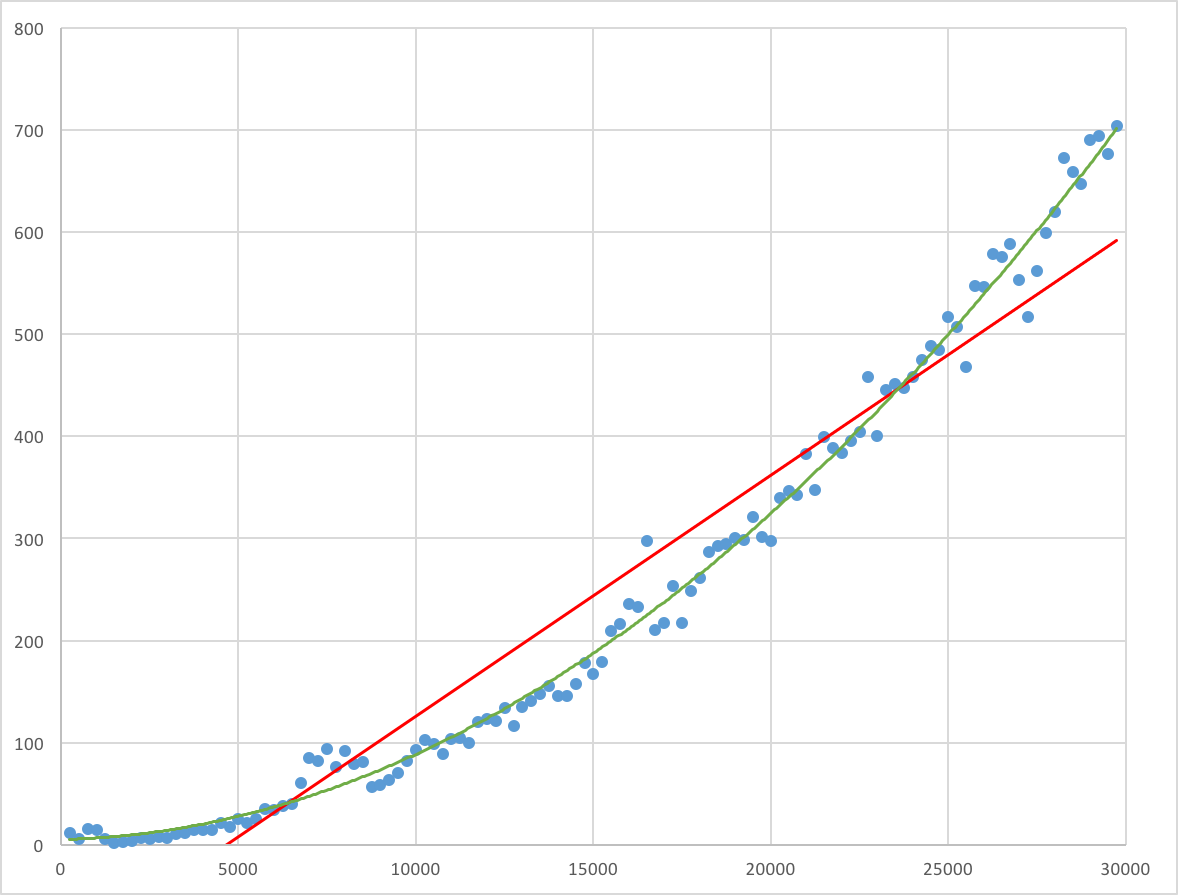
\includegraphics[width=100mm]{./img/selection_sort_linear_trendline.png}}}
	\caption{Linear regression model of selection sort runtime samples.}
	\label{fig:selection_sort_linear_trendline}
\end{figure}

The model can then be used to formulate simple predictions, $a'x + b'$ being the prediction for \textit{input descriptor} $x$. Next, we need to find a way how to determine the certainty of the prediction to be able to select the best function with given certainty using a set of these models.

\subsubsection{Confidence interval based selection from two functions}
\label{subsubsec:confidence_interval_selection}

Suppose we have the linear regression model \(h'(x) = a' x + b'\) that approximates the function $h(x) = ax + b$ constructed using \(n\) data samples \(x_i, y_i\) (in our case, \(x_i\) are the \textit{input descriptors} and \(y_i\) are the run times). If we assume that the errors $\varepsilon_i = y_i - h'(x_i)$ of our sample from the regression model values are random variables with normal distribution, we can perform some observation about the model.

Firstly, the standard errors $se(b')$ and $se(a')$ of the intercept $b'$ and the slope $a'$ can be derived from the model. In addition, the statistics $t_a = \frac{a' - a}{se(a')}$ and $t_b = \frac{b' - b}{se(b')}$ have a t-distribution with $n-2$ degrees of freedom. This means that we are able to construct confidence intervals and perform t-tests for $a$ and $b$. The default tests hypotheses have the following form:

\[H_0:\; a = a_0\]
\[H_1:\; a \neq a_0 \]

We basically test equality of $a$ (or $b$) and a fixed value $a_0$ (or $b_0$) - this test can be used to verify if the data have a specific linear relation. If we put $a_0 = 0$, we can find out whether the observations $y_i$ are constant. 

None of these tests and statistics, however, allows us to test the certainty of the prediction - we need to consider both the intercept and the slope estimation certainty, and, in addition, the distance of the $x$ we want the prediction for from the mean $\bar{x}$. The reason is that if we commit an error in the slope estimation $a'$, the corresponding error in predictions increases with the distance from $\bar{x}$. 

With these facts, a confidence interval on level $1 - \alpha$ for the mean of the actual values ($y$) for $x$ can be constructed. According to \cite{weiss_introductory_2010}, the width of the interval is the following:

%TODO: Change the text to "mean prediction interval"

\[
w_{x, \alpha} = t_{n - 2}(1-\frac{\alpha}{2}) s_e\sqrt{\frac{1}{n} + \frac{(x - \bar{x})^2}{ \sum_{i = 1}^{n} (x_i - \bar{x})^2 }}
\]

where \(\bar{x}\) is the mean of \(x_i\), $t_{n - 2}(1-\frac{\alpha}{2})$ is the $(1-\frac{\alpha}{2})$-th quantile of \textit{t-distribution} with $n-2$ degrees of freedom, and $s_e$\footnote{Standard error of the estimate} can be computed as:

\[s_e = \sqrt{\frac{SSE}{n-2}}\]

and

\[SSE = \sum_{i = 1}^{n} \varepsilon_i^2  =  \sum_{i = 1}^{n} (y_i - y_i')^2 \]

for \(y_i' = h'(x_i)\).

It now holds for any $x$ that the mean of $y = h(x)$ lies in $[a'x + b' \pm w_{x, \alpha}]$ with probability $(1-\alpha)$.

Now in the situation where we have two regression models and we want to find the best prediction of $x$, we can construct these confidence intervals for both models and:

\begin{itemize}
	\item If the intervals do not overlap, the predictions have at least a $(1 - \alpha)^2$ probability of correctly setting the order, i.e. the worse prediction actually being the worse function
	\item If the intervals overlap, there is a non-trivial chance of the predictions being mixed up by error
\end{itemize}

In the first case, we can decide that one function is significantly better and select it. In the second case, we cannot decide with given certainty.

\subsubsection{Confidence interval based selection from multiple functions}

The described method allows us to decide between two functions with given certainty. Now, when choosing among $n$ functions with regressions $h'_1, \dots, h'_n$ for given $x$, we are looking for the $k$ for which the following holds:

\begin{itemize}
	\item The confidence interval on level $(1-\alpha)$ for prediction $h'_k(x)$ does not overlap with any other of the confidence interval for prediction.
	\item $\forall j \ne k: h'_k(x) < h'_j(x)$
\end{itemize}

It can be done by constructing all the regression models and then $\forall i$ performing the comparison described in \ref{subsubsec:confidence_interval_selection} of $h_i$ with $h_j, \forall j \ne i$. If $h_i$ is better than all of the $h_j$, we can choose the corresponding function.

The strength of this decision is influenced by the fact that we perform multiple confidence interval constructions - the errors an error in any of them can influence the result of the selection, se the significance gets lower in general. If we wanted the results to be precise, we would have to perform the correction of the significance level $\alpha$. Just like in \ref{subsec:t_test_multiple}, we will leave the significance correction analysis as a potential future work.

\subsubsection{Selection algorithm}

The strategy is parametrized by the selection significance level $\alpha$ and by the secondary strategy to be used in case of decision failure.

\begin{algorithmic}[1] % The number tells where the line numbering should start
	\INPUT Historical data vectors $d_1,...,d_n$ where $d_i = [(x_{i,1}, y_{i,1}),...,(x_{i,l_i}, y_{i,l_i})]$, \textit{input descriptor} $x$
	\For{$i=1$ to $n$}
	\State $r_i \gets$ createRegression($d_i$) \Comment{Uses the least squares method}
	\EndFor
	\For{$i = 1$ to $n$}
	\State $better \gets$ true
	\For{$j = 1$ to $n$, $j \ne i$}
	\State $(k_1, l_1) \gets$ predictionInterval($r_i, x, \alpha$)
	\State $(k_2, l_2) \gets$ predictionInterval($r_j, x, \alpha)$
	\If{$(k_1, l_1)$ overlaps $(k_2, l_2)$ or $k_1 > k_2$}
	\State $better \gets$ false
	\EndIf
	\EndFor
	\If{$better$}
	\State \Return{$i$}
	\EndIf
	\EndFor
	\State \Return{useSecondaryStrategy($d_1,\dots,d_n, x$)}
\end{algorithmic}

\subsection{Window-bound linear regression}
\label{subsec:window_bound_regression}

To be able to apply the strategy described in section \ref{subsec:simple_linear_regression} on a wider variety of functions, a simple approach to lower the approximation errors can be taken. Instead of creating a regression model for the entire set of historical measurements at once, we can split it into more subsets and create different regressions for them. Figure \ref{fig:window_examples} shows ranges $5000$ to $10000$, $10000$ to $15000$ and $15000$ to $20000$ of the input sizes of the data from \ref{fig:selection_sort_linear_trendline}. As we can observe from the second and third range, the data tend to be much closer to the linear regression line. The first range shows that a less significant fluctuation in the entire set has a lot bigger impact on the model in a smaller subset.

\begin{figure}[h!]
	\captionsetup{justification=centering,margin=0.5cm}
	\centerline{\mbox{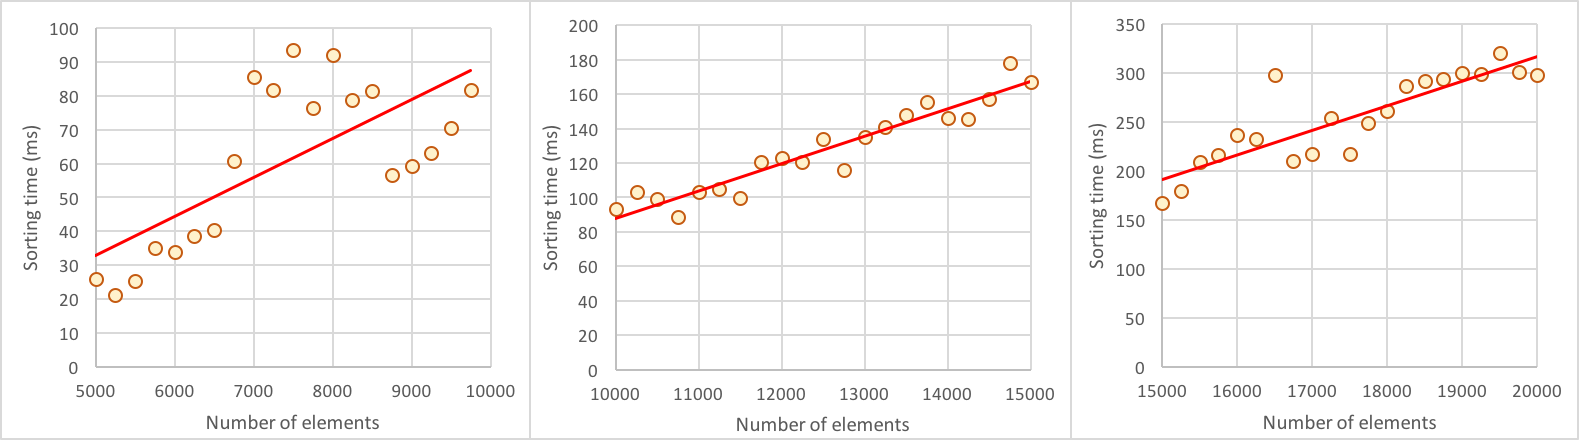
\includegraphics[width=150mm]{./img/window_examples.png}}}
	\caption{Examples of subsets of the data from figure \ref{fig:selection_sort_linear_trendline} with corresponding linear regressions.}
	\label{fig:window_examples}
\end{figure}

When selecting a function for a specific \textit{input descriptor} $x$, a window around its value of specific width $w$ can be created and the regression model built using the data from the said window. We do it by selecting only the historical samples $(x_k, y_k)$ where $\abs{x_k - x} < w$ when constructing the regression.

There are multiple ways how to decide on the window width $w$. Using a fixed number across all the functions and all the data samples would not be recommendable, as the functions can vary in their \textit{input descriptors} by orders of magnitude. The width could be derived as a fraction of the width of the whole data set: $w = \frac{max(x_i) - min(x_i)}{p}$, where $p$ would represent in how many parts we want it to be split. 

More flexible approach is to dynamically determine the $p$. Suppose we want the average window to contain $r$ records. We find out what is the average distance between two neighboring records as $d =  \frac{max(x_i) - min(x_i)}{n - 1}$ and then set the $w = r * d$. This way, the window size will always be adapted to the density of the dataset.

The window limitation might seem similar to the grouping described in \ref{subsec:grouping}, but there are two major differences. First, the windows are based on the \textit{input descriptor}, whereas the \textit{group selector} might use different features of the input. And second, the groups are deterministic and do not move with the \textit{input descriptor} and change their size based on historical data. Both these concept can be used at the same time.

\subsubsection{Selection algorithm}

The strategy is parametrized by the selection significance level $\alpha$ and by the average record count per window $avg$.

\begin{algorithmic}[1] % The number tells where the line numbering should start
	\INPUT Historical data vectors $d_1,...,d_n$ where $d_i = [(x_{i,1}, y_{i,1}),...,(x_{i,l_i}, y_{i,l_i})]$, \textit{input descriptor} $x$
	\For{$i=1$ to $n$}
	\State $dist \gets (max(x_{i,j}) - min(x_{i,j})) / (l_i-1)$
	\State $w \gets dist * avg$
	\State $d'_i \gets [(x_{i,j}, y_{i, j}); \forall j: \abs{x_{i,j} - x} \leq w/2]$
	\EndFor
	\State \Return{useLinearRegressionStrategy($d'_1,...,d'_n, x$)}
\end{algorithmic}

\subsection{Local regression}
\label{subsec:local_regression}

The approach explained in \ref{subsec:window_bound_regression} can be extended further - the locally constructed linear regression models might be used to build up a model for the entire data set. This leads to a model that is non-linear, i.e., the function that approximates the original data relation is not a linear function.

One possible regression method that behaves this way is \textit{LOESS} (Local Regression, \cite{cleveland_locally_1988,cleveland_regression_1988,cleveland_computational_1991}). It uses techniques similar to the least-square regression on local subsets of the data set, and then smooths up the resulting curve. The output is a \textit{Loess Curve}, an artificially constructed function that does not necessarily have to be expressed by a formula. This is one of the advantages of the model - the original relation between \textit{input descriptors} and the run times did not have to be expressed by a simple function in order to be captured correctly.

The \textit{LOESS} model can be used to predict the function run times. It is, however, a lot more complicated to derive the prediction confidence intervals. Therefore, only the values will be used in this selection strategy, which could lead to some wrong decisions.

There are other disadvantages of this strategy as well. First of all, the entire local regression model has to be recomputed whenever there is a new record in the dataset, the model cannot be simply updated like the \textit{simple linear regression}. Secondly, it is much more computationally complex and the model construction takes non-trivial time, so it has a negative impact on the framework overhead, especially when used with short and simple functions. The last downside of \textit{local regression} is its inability to predict further behavior past the minimum and maximum data sample.

\subsubsection{Selection algorithm}

The strategy is parametrized by the secondary strategy to be used in case of decision failure.

\begin{algorithmic}[1] % The number tells where the line numbering should start
	\INPUT Historical data vectors $d_1,...,d_n$ where $d_i = [(x_{i,1}, y_{i,1}),...,(x_{i,l_i}, y_{i,l_i})]$, \textit{input descriptor} $x$
	\For{$i=1$ to $n$}
	\State $m_i \gets$ interpolateLoess($d_i$)
	\State $p_i \gets$ predictValue($m_i, x$)
	\If{$p_i = NaN$}\Comment{The prediction can fail}
	\State\Return{useSecondaryStrategy($d_1,\dots,d_n, x$)}
	\EndIf
	\EndFor
	\State\Return{$argmin(p_i)$}
\end{algorithmic}

\subsection{Window-bound t-test}
\label{subsec:window_bound_t_test}

The mean based t-test selection strategy described in sections \ref{subsec:t_test_two} and \ref{subsec:t_test_multiple} works under the assumption that the run times of a specific function have a normal distribution, and the prediction of run time is simply the mean of all the times measured. This could be true only for the functions with constant complexity - whenever the function run time depends on the input, the samples measured have their distribution influenced by the distribution of the inputs.

\begin{figure}[h!]
	\captionsetup{justification=centering,margin=0.5cm}
	\centerline{\mbox{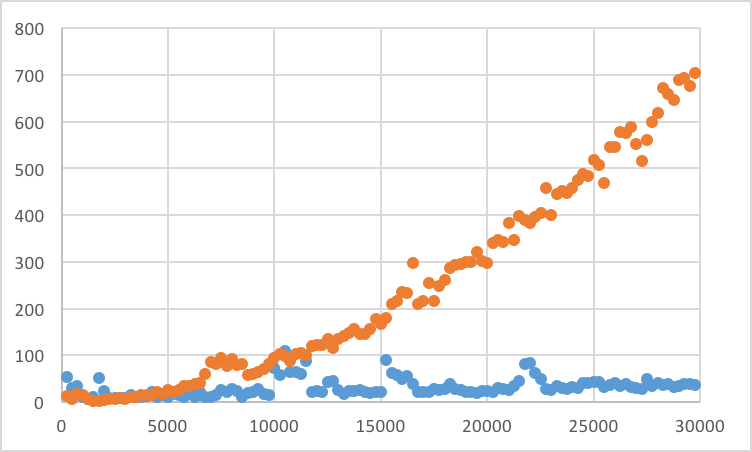
\includegraphics[width=100mm]{./img/quick_vs_selection.png}}}
	\caption{Run times of quick sort algorithm (dark dots) and selection sort algorithm (light dots) by input size.}
	\label{fig:quick_vs_selection}
\end{figure}

\begin{figure}[h!]
	\captionsetup{justification=centering,margin=0.5cm}
	\centerline{\mbox{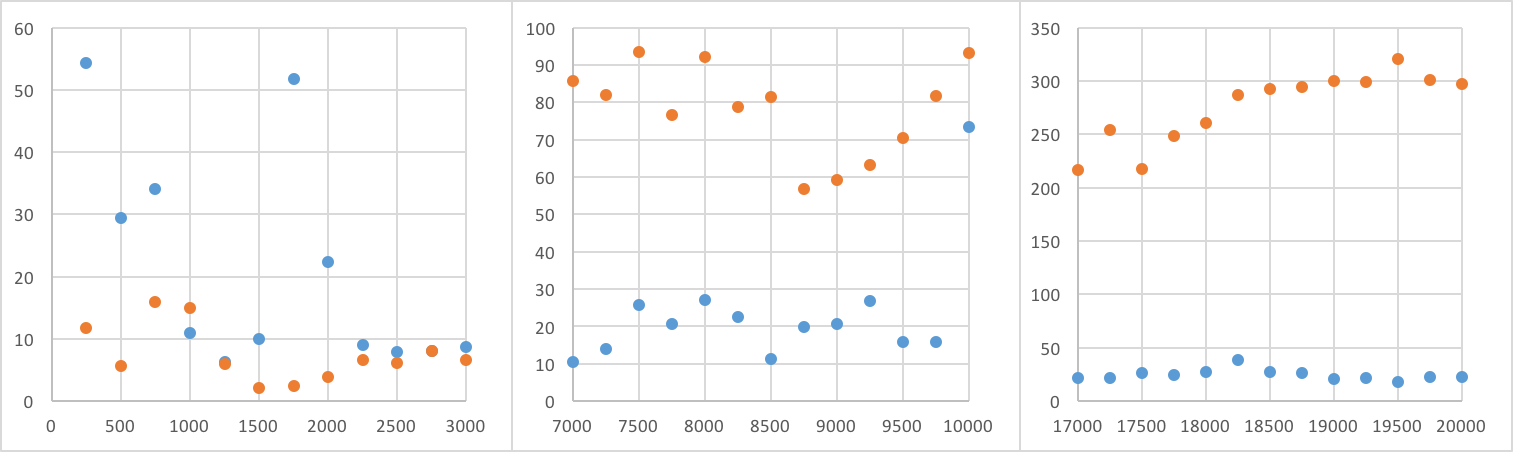
\includegraphics[width=150mm]{./img/window_t_test_examples.png}}}
	\caption{Examples of subsets of the data from figure \ref{fig:quick_vs_selection}}
	\label{fig:window_t_test_examples}
\end{figure}

If we wanted to use the t-test strategy on the functions with non-constant complexity, the same approach as with the \textit{simple linear regression} can be taken. Instead of assuming that the relation in the small window is linear, we want it to be constant and normally distributed. We can then predict the run time using the mean of the measurements from within a very small range of \textit{input descriptor} values. Consequently, it is extremely important to keep the window size as small as possible, so that these assumptions held at least approximately. The t-test significance levels and strengths will be approximate as well, but our goal is to get reasonable selection behavior, we do not need to be precise.

Figure \ref{fig:quick_vs_selection} shows the run times measured for the quick sort and selection sort algorithms on random arrays of sizes between $0$ and $30000$. Obviously, there is a relation to the input size, so the simple t-test should not be applied in this case. In figure \ref{fig:window_t_test_examples}, there are the same data in three different windows - $0$ to $3000$, $7000$ to $10000$ and $17000$ to $20000$. As we can see, in a window of this size, the run times are almost constant and the random fluctuations are more significant than the actual relation to the input size. We can apply the t-test as described in sections \ref{subsec:t_test_two} and \ref{subsec:t_test_multiple} to these windows and consider the result to be relevant enough with respect to the input.

The window sizes can be determined in a similar way as in section \ref{subsec:window_bound_regression}. If we reduce it to a constant 0, we will get a technique in which only the results for inputs with the same descriptor are tested. When there are none, we refuse to select and wait until data are gathered. This might be useful in cases where we know that the function will be called repeatedly on a limited set of input variants, and basically rules out the prediction factor, as we need to have actual observation for each input before making any conclusions. Similar approach is taken in \cite{bulej_performance_2012}. The same goal, however, can be achieved more efficiently using the grouping mechanism (see \ref{subsec:grouping}).

\subsubsection{Selection algorithm}

The strategy is parametrized by the selection significance level $\alpha$ and by the average record count per window $avg$.

\begin{algorithmic}[1] % The number tells where the line numbering should start
	\INPUT Historical data vectors $d_1,...,d_n$ where $d_i = [(x_{i,1}, y_{i,1}),...,(x_{i,l_i}, y_{i,l_i})]$, \textit{input descriptor} $x$
	\For{$i=1$ to $n$}
	\State $dist \gets (max(x_{i,j}) - min(x_{i,j})) / (l_i-1)$
	\State $w \gets dist * avg$
	\State $d'_i \gets [(x_{i,j}, y_{i, j}); \forall j: \abs{x_{i,j} - x} \leq w/2]$
	\EndFor
	\State \Return{useTTestStrategy($d'_1,...,d'_n$)}
\end{algorithmic}

\subsection{Whitebox model construction}

The methods that were described so far are examples of the blackbox techniques - they do not analyze the function itself, the models are based only on the relation of the run times and the \textit{input descriptors}. 

The techniques used in the research projects focused on formulating accurate predictions about program run times (like \cite{goldsmith_measuring_2007,chun_mantis:_2010,huang_predicting_2010}) often build the model using more detailed information about every run. These extra data can be obtained by examining and instrumenting the function code. Key structures (loops, branches, method invocation, ...) can be identified and execution counts can be tracked. Then, a model that captures the relation between the input features, the described structure execution counts and the run time can be constructed. This added dimension might lead to more accurate model and therefore better predictions.

%TODO: Add reference / bibliography
In \cite{chun_mantis:_2010}, a Mantis framework for high accuracy program performance prediction was implemented. The basic principles are similar to the approach described above. It was tested on a series of data gathered from runs of the ImageJ application, and compared with a blackbox prediction model based on interpolating a polynomial of degree three. The prediction error of the whitebox approach was 5.5\%, the blackbox approach error rate reached more than 35\%.
%TODO: Add results?

This approach has, however, a few problems concerning the intended use cases of our framework. The model will not improve the predictions if the majority of the execution time is spent waiting on an I/O operation. Specifically, it will not help with any of the cases where we are selecting a database query, remote server to connect to, etc. In addition, it would require the method code to be instrumented at runtime, which would lead, together with the model construction, to a significant overhead.

For these reasons and because of the complexity, the whitebox model was not implemented in the framework, but it represents a potential future work that could be done on the topic.

\section{Strategy comparison}
\label{sec:strategy_comparison}

In general, the input based strategies do not handle well more historical results for the same \textit{input descriptor}, and are impossible to use when there is none specified. The following rules should be used to decide between input based and mean based strategies:

\begin{itemize}
	\item \textbf{Dependency on the input} \\
	If the function does not have any input, or the input does not affect the expected run time (the complexity is constant), mean based strategies should be used.
	\item \textbf{Expected input values} \\
	If the function is expected to be invoked with a discrete and very limited set of inputs, mean based strategy is preferred. On the other hand, if the function will be called repeatedly with randomly distributed inputs, the input based strategies are a better choice.
\end{itemize}

Considering these facts, the framework will contain both an input based and a mean based strategy, and will automatically use the input based one if the user specified an \textit{input descriptor}, and the mean based one otherwise. The user will be able to override this choice if he wants.

The actual strategies used should be easily replaceable, but some have to be chosen as default for the common uses. Therefore, a practical comparison of the selection success rate and overheads of the strategies that were described and implemented follows.

\subsection{Input based strategies success rates}
\label{subsec:input_based_strategies_success}

To compare the efficiency of the selection strategies, we will perform two tests. The first one will be based on an artificial function with linear complexity defined by the following lambda expression:

\lstset{style=Scala}
\begin{lstlisting}
i => {
  val j = (i * k).toInt
  var acc = 0
  Seq.range(0, j).foreach(l => {
    acc = acc + (l * Random.nextInt(1000))
  })
  acc
}
\end{lstlisting}

Where \inlinecode{i} is the input of the function and \inlinecode{k} is a constant factor which can be used to slow the function down.

Analogically, we will define a quadratic function (using a similar lambda, only with second line replaced by \inlinecode{val j = (i * i * k).toInt}).

Now, the test will be based on combining two instances of the same function\footnote{Note that the actual implementation requires either using two different lambdas, or using custom identifiers, more on that topic in section \ref{subsec:function_identifiers}}, one with $k=1$ and the other with some $k>1$, perform a series of runs and track how many times will the selection strategy choose the worse one (i.e. the $k>1$ one).

For each test, we will generate 100 sequences, each one containing 200 integers between 100000 and 500000 in case of the linear function, or 100 and 500 for the quadratic function. One sequence will represent one test run - the measurement history will be flushed and the function will be invoked on the members of the sequence one by one. The strategies are set in the way that the first 60 runs will use a round-robin selection to gather 30 data samples for each function before starting the actual selection. It means that the strategy should perform 140 selections for each test run. We are going to count how many times the worse function is selected. The baseline solution in this case would be to keep using the round-robin technique, which would lead to the worse function being selected 50\% of the time, 70 times out of 140.

Now, we will use the following values for $k$: 4, 2, 1.5, 1.2, 1.1, 1.01, and the following selectors:
\begin{itemize}
	\item Window-bound t-test (WBTT) with $\alpha$ set to 0.05 and 0.25
	\item Linear regression (LR) with $\alpha$ set to 0.05 and 0.25
	\item Window-bound linear regression (WBLR) with $\alpha$ set to 0.05 and 0.25
	\item Local regression (LOESS)
\end{itemize}

For each combination, all 100 test runs were performed and an average percentage of the worse function selection was computed, the results for the linear function can be seen in table \ref{tab:strategy_comparison} and for the quadratic function in table \ref{tab:strategy_comparison_quadratic}. A surprising fact might be the overall better results for the non-linear case, which should be more difficult to model. The reason for this fact is that there is a dramatically lower range of inputs (100 to 500 instead of 100000 to 500000) in order to keep the test run time realistic. In addition, the run time differences between individual inputs grows much faster, so the error factor involved does less damage to the model. In general, it seems that functions with faster-growing complexities get more precise predictions.


\begin{table}[h!]
	\captionsetup{justification=centering,margin=0.5cm}
	\centering
	\bgroup
	\def\arraystretch{1.5}%
	\begin{tabular}{|l|r|r|r|r|r|r|r|}
		\hline
		\textbf{}      & \multicolumn{1}{c|}{\textbf{\begin{tabular}[c]{@{}c@{}}WBTT\\ (0.05)\end{tabular}}} & \multicolumn{1}{c|}{\textbf{\begin{tabular}[c]{@{}c@{}}LR\\ (0.05)\end{tabular}}} & \multicolumn{1}{c|}{\textbf{\begin{tabular}[c]{@{}c@{}}WBLR\\ (0.05)\end{tabular}}} & \multicolumn{1}{c|}{\textbf{\begin{tabular}[c]{@{}c@{}}WBTT\\ (0.25)\end{tabular}}} & \multicolumn{1}{c|}{\textbf{\begin{tabular}[c]{@{}c@{}}LR\\ (0.25)\end{tabular}}} & \multicolumn{1}{c|}{\textbf{\begin{tabular}[c]{@{}c@{}}WBLR\\ (0.25)\end{tabular}}} & \multicolumn{1}{c|}{\textbf{LOESS}} \\ \hline
		\textbf{1.01x} & 52.4\%                                                                              & 49.6\%                                                                            & 51.5\%                                                                              & 47.1\%                                                                              & 49.6\%                                                                            & 50.1\%                                                                              & 43.6\%                              \\ \hline
		\textbf{1.1x}  & 49.4\%                                                                              & 48.5\%                                                                            & 37.2\%                                                                              & 33.7\%                                                                              & 44.6\%                                                                            & 33.5\%                                                                              & 6.2\%                               \\ \hline
		\textbf{1.2x}  & 40.1\%                                                                              & 46.0\%                                                                            & 29.0\%                                                                              & 26.3\%                                                                              & 41.6\%                                                                            & 27.8\%                                                                              & 3.5\%                               \\ \hline
		\textbf{1.5x}  & 30.2\%                                                                              & 38.9\%                                                                            & 13.9\%                                                                              & 13.7\%                                                                              & 25.6\%                                                                            & 9.9\%                                                                               & 2.9\%                               \\ \hline
		\textbf{2x}    & 17.6\%                                                                              & 25.4\%                                                                            & 7.8\%                                                                               & 4.3\%                                                                               & 14.4\%                                                                            & 4.7\%                                                                               & 2.4\%                               \\ \hline
		\textbf{4x}    & 2.9\%                                                                               & 15.7\%                                                                            & 5.0\%                                                                               & 0.1\%                                                                               & 9.7\%                                                                             & 2.7\%                                                                               & 2.5\%                               \\ \hline
	\end{tabular}
	\egroup
	\caption{Percentage of times the strategy selected the worse one out of two linear functions (average from 100 test runs, each containing 140 selections).}
	\label{tab:strategy_comparison}
\end{table}

\begin{table}[h!]
	\captionsetup{justification=centering,margin=0.5cm}
	\centering
	\bgroup
	\def\arraystretch{1.5}%
	\begin{tabular}{|l|r|r|r|r|r|r|r|}
		\hline
		\multicolumn{1}{|c|}{\textbf{}} & \multicolumn{1}{c|}{\textbf{\begin{tabular}[c]{@{}c@{}}WBTT\\ (0.05)\end{tabular}}} & \multicolumn{1}{c|}{\textbf{\begin{tabular}[c]{@{}c@{}}LR\\ (0.05)\end{tabular}}} & \multicolumn{1}{c|}{\textbf{\begin{tabular}[c]{@{}c@{}}WBLR\\ (0.05)\end{tabular}}} & \multicolumn{1}{c|}{\textbf{\begin{tabular}[c]{@{}c@{}}WBTT\\ (0.25)\end{tabular}}} & \multicolumn{1}{c|}{\textbf{\begin{tabular}[c]{@{}c@{}}LR\\ (0.25)\end{tabular}}} & \multicolumn{1}{c|}{\textbf{\begin{tabular}[c]{@{}c@{}}WBLR\\ (0.25)\end{tabular}}} & \multicolumn{1}{c|}{\textbf{LOESS}} \\ \hline
		\textbf{1.01x}                  & 52.3\%                                                                              & 49.4\%                                                                            & 44.6\%                                                                              & 50.5\%                                                                              & 50.3\%                                                                            & 49.5\%                                                                              & 44.6\%                              \\ \hline
		\textbf{1.1x}                   & 44.9\%                                                                              & 43.1\%                                                                            & 28.9\%                                                                              & 33.3\%                                                                              & 37.8\%                                                                            & 26.2\%                                                                              & 7.4\%                               \\ \hline
		\textbf{1.2x}                   & 38.2\%                                                                              & 38.1\%                                                                            & 16.3\%                                                                              & 17.8\%                                                                              & 31.2\%                                                                            & 15.7\%                                                                              & 4.0\%                               \\ \hline
		\textbf{1.5x}                   & 16.6\%                                                                              & 28.7\%                                                                            & 8.4\%                                                                               & 7.9\%                                                                               & 18.5\%                                                                            & 6.4\%                                                                               & 2.5\%                               \\ \hline
		\textbf{2x}                     & 8.8\%                                                                               & 20.0\%                                                                            & 4.1\%                                                                               & 2.7\%                                                                               & 13.4\%                                                                            & 2.4\%                                                                               & 2.3\%                               \\ \hline
		\textbf{4x}                     & 3.5\%                                                                               & 19.6\%                                                                            & 3.0\%                                                                               & 0.1\%                                                                               & 14.6\%                                                                            & 1.5\%                                                                               & 2.3\%                               \\ \hline
	\end{tabular}
	\egroup
	\caption{Percentage of times the strategy selected the worse one out of two quadratic functions (average from 100 test runs, each containing 140 selections).}
	\label{tab:strategy_comparison_quadratic}
\end{table}

As to the individual strategies, it might be unexpected that the linear regression has quite poor results, even in the case where the original function complexities were linear. Almost $16\%$ of selections of a function that is four times slower in the $\alpha = 0.05$ case. This is caused by the fact that eventual measurements with extreme deviations influence the whole model, not just a local part of it, which might lead to an eventual series of wrong decisions. Therefore, linear regression strategy is not recommended to be used in general.

On the other hand, the absolute winner is the local regression, which is able to maintain extremely low error rates ($6.2\%$ for the linear functions, $7.4\%$ for the quadratic functions) for the second-minimal case $k=1.1$, and push it even lower with growing $k$. Neither one of the other strategies got below $15\%$ not only for $k=1.1$, but even for $k=1.2$.

The window-bound strategies are somewhere in the middle - they perform very well for higher $k$ ($2, 4$), which is the main concern, and reasonably for the other sizes. The main difference between them being that the window-bound linear regression improves steadily with growing $k$, whereas the window-bound t-test reaches better results for the largest $k=4$, but improves dramatically at the end and has worse results for lower $k$.

We can see that in all the cases, lowering the selection significance (by increasing the $\alpha$) can lead to slightly better results overall, especially for larger values of $k$. The success of local regression, which does not employ certainty in the decision making process, supports this observation. It seems that the assumption of selection errors having a bad influence on the model and leading to chains of bad decisions was not confirmed by this test. It might be, however, different for real-life scenarios with more variable run times, environment changes, etc., and we should keep that in mind and be careful when lowering the $\alpha$ for better selection results.

\subsection{Mean based strategies success rates}

Similarly to the input based strategies, we are going to perform a selection success rate test for the mean based strategies. As we need only a function with fixed non-trivial execution time with a possibility to slow it down a little, we are going to reuse the linear function from section \ref{subsec:input_based_strategies_success}, fixing its input to 200000. Again, we are going to combine an instance of the non-slowed function with the instances of function slowed by a factor $k$. 

The values 2, 1.5, 1.2, 1.1, 1.01 will be used for $k$, along with the following selectors:
\begin{itemize}
	\item T-test (TT) with $\alpha$ set to 0.05 and 0.25
	\item U-test (UT) with $\alpha$ set to 0.05 and 0.25
\end{itemize}

For each combination of $k$ and a selector, 100 test runs will be performed, each one consisting of invoking the described combined function 200 times and removing all the history records afterwards.

The results can be seen in table \ref{tab:strategy_comparison_mean_based}. It might seem obvious that the u-tests deliver better results, and again, lowering the $\alpha$ improves the result as well. In order to get more insight into the results, we should take into account another factor - the number of test runs, where the overall success rate was worse than the baseline success rate, i.e. the $50\%$ of the round-robin selection. This is shown in the table \ref{tab:strategy_comparison_mean_based_worse_runs}.

\begin{table}[h!]
	\captionsetup{justification=centering,margin=0.5cm}
	\centering
	\bgroup
	\def\arraystretch{1.5}%
	\begin{tabular}{|l|r|r|r|r|}
		\hline
		& \multicolumn{1}{c|}{\textbf{\begin{tabular}[c]{@{}c@{}}TT\\ (0.05)\end{tabular}}} & \multicolumn{1}{c|}{\textbf{\begin{tabular}[c]{@{}c@{}}UT\\ (0.05)\end{tabular}}} & \multicolumn{1}{c|}{\textbf{\begin{tabular}[c]{@{}c@{}}TT\\ (0.25)\end{tabular}}} & \multicolumn{1}{c|}{\textbf{\begin{tabular}[c]{@{}c@{}}UT\\ (0.25)\end{tabular}}} \\ \hline
		\textbf{1.01x} & 49.8\%                                                                            & 49.5\%                                                                            & 49.8\%                                                                            & 47.1\%                                                                            \\ \hline
		\textbf{1.1x}  & 46.6\%                                                                            & 27.0\%                                                                            & 39.1\%                                                                            & 25.5\%                                                                            \\ \hline
		\textbf{1.2x}  & 42.2\%                                                                            & 18.5\%                                                                            & 25.6\%                                                                            & 14.3\%                                                                            \\ \hline
		\textbf{1.5x}  & 11.6\%                                                                            & 0.0\%                                                                             & 2.6\%                                                                             & 0.2\%                                                                             \\ \hline
		\textbf{2x}    & 1.9\%                                                                             & 0.0\%                                                                             & 0.0\%                                                                             & 0.0\%                                                                             \\ \hline
	\end{tabular}
\egroup
\caption{Percentage of times the strategy selected the worse one out of two constant functions (average from 100 test runs, each containing 140 selections).}
\label{tab:strategy_comparison_mean_based}
\end{table}

\begin{table}[h!]
	\captionsetup{justification=centering,margin=0.5cm}
	\centering
	\bgroup
	\def\arraystretch{1.5}%
	\begin{tabular}{|l|r|r|r|r|}
		\hline
		& \multicolumn{1}{c|}{\textbf{\begin{tabular}[c]{@{}c@{}}TT\\ (0.05)\end{tabular}}} & \multicolumn{1}{c|}{\textbf{\begin{tabular}[c]{@{}c@{}}UT\\ (0.05)\end{tabular}}} & \multicolumn{1}{c|}{\textbf{\begin{tabular}[c]{@{}c@{}}TT\\ (0.25)\end{tabular}}} & \multicolumn{1}{c|}{\textbf{\begin{tabular}[c]{@{}c@{}}UT\\ (0.25)\end{tabular}}} \\ \hline
		\textbf{1.01x} & 0                                                                                 & 1                                                                                 & 19                                                                                & 7                                                                                 \\ \hline
		\textbf{1.1x}  & 0                                                                                 & 15                                                                                & 5                                                                                 & 20                                                                                \\ \hline
		\textbf{1.2x}  & 0                                                                                 & 15                                                                                & 4                                                                                 & 13                                                                                \\ \hline
		\textbf{1.5x}  & 0                                                                                 & 0                                                                                 & 0                                                                                 & 0                                                                                 \\ \hline
		\textbf{2x}    & 0                                                                                 & 0                                                                                 & 0                                                                                 & 0                                                                                 \\ \hline
	\end{tabular}
\egroup
\caption{The number of test runs (out of 100) where the strategy had a success rate worse than 50\%.}
\label{tab:strategy_comparison_mean_based_worse_runs}
\end{table}

It looks like the t-test is more conservative, it refuses to make the decision more often, which leads to switching the functions in the round-robin fashion. On the other hand, the u-test risks more, which leads to better results overall, but there are some runs that are very bad - for $k=1.2$, $15$ runs out of $100$ were worse than $50\%$, and $10$ out of these $15$ runs had a $0\%$ success rate, which means that the model selected the worse function every time.

The conclusion from the observations is that employing u-test (or increasing the $\alpha$) increases the expected success rate in a common case, but brings a non-trivial risk of constructing a wrong model which leads to a sequence of errors that might last very long.

\subsection{Strategy performance}
\label{subsec:strategy_perf}

When deciding for one of the strategies, there is another concern that we should keep in mind. The strategies tend to be quite complex and their execution time might become non-trivial. As they need to process the entire run history of each of the functions, their selection times increase over time, as more historical measurements are collected.

For some of the strategies, it is possible to compute and cache the statistical data in advance, at the moment of storing newly measured data, allowing them to avoid processing all the records again during the selection. From our strategy list, this is possible to be done for the linear regression and the t-tests. Unfortunately, neither the window-bound strategies, nor the local regression support this approach.

To compare the practical overheads, we ran the selection using each of the strategies 20000 times in a row (while evaluating the runs and adding new data in the process) for the task of deciding between quick sort and selection sort algorithm on sequences of 0 to 2000 numbers. The window-bound strategies had the window size calculated to contain 25 records in average. The resulting averages of selection strategy run times are in table \ref{tab:strategy_execution_comparison}.

\begin{table}[h!]
	\captionsetup{justification=centering,margin=0.5cm}
	\centering
	\bgroup
	\def\arraystretch{1.5}%
	\begin{tabular}{|l|r|r|}
		\hline
		\textbf{}                  & \multicolumn{1}{l|}{\textbf{Not cached}} & \multicolumn{1}{l|}{\textbf{Cached}} \\ \hline
		\textbf{Linear regression} & 1.68                                     & 0.15                                 \\ \hline
		\textbf{Window-bound LR}   & 0.91                                     & -                                  \\ \hline
		\textbf{Window-bound TT}   & 0.72                                     & -                                  \\ \hline
		\textbf{LOESS}             & 57.47                                    & -                                  \\ \hline
		\textbf{T-test}            & 1.32                                     & 0.10                                 \\ \hline
		\textbf{U-test}            & 5.91                                     & -                                  \\ \hline
	\end{tabular}
\egroup
\caption{Average strategy selection time (in ms) in a sequence of 20000 consecutive selections.}
\label{tab:strategy_execution_comparison}
\end{table}


The results are showing that local regression has extremely high run times that can grow above 50 milliseconds for situations with larger number of historical observations. An overhead of this size on every selection would be too high for most common usages, so the local regression strategy, even though it has the best success rate, should be used with extreme caution and only in cases where it is clear that overhead this high cannot damage the system performance. 

As for the remaining strategies, it seems that caching speeds up the selection a little more than 10 times for this number of runs. The window-bound strategies cannot be improved by the caching (as the relevant statistics are different for every window), but they have the lowest execution time of all the strategies without cache, and therefore are very usable for the input based case. Regarding the mean based strategies, the t-test is almost 5 times faster than the u-test in the non-cached version, and more than 50 times faster when using the cache, so it is clearly a better choice if performance is the main concern.

\section{Invocation policies}
\label{sec:policies}

The selection process and all the strategies described in sections \ref{sec:mean_based_strategies} and \ref{sec:input_based_strategies} are quite complex and have non-trivial overhead, especially after collecting a large amount of historical data, as discussed in section \ref{subsec:strategy_perf}. In a common scenario where we expect the system to come to a decision about the best function (either overall, or separately for every group), it would be suitable if we could stop the selection process at a certain point and keep using only the most favored function with no extra overhead. Or, to use it most of the time, with only occasional attempts at the selection in order to detect possible changes in the system (response times, I/O operation duration, etc.).

Similarly, it might be desirable to control the overhead time spent on the selection, or, in general, on invoking the functions using selection (which might lead to a bad decision), either per a specific time period, or with respect to a specific action of the system (user request, processing unit, etc.). All of these decisions should be taken at a higher level than the run time history analysis performed by the selection strategies.  

\textit{Invocation policies} are a concept that tries to address these cases, with the main purpose of lowering its invocation overhead. Every combined function has an \textit{invocation policy} associated with it. In the function selection chain, the policy gets evaluated right after invoking the combined function and is supposed to quickly decide how to proceed with the invocation. There might be scenarios where a faster ways could be taken without even using any of the strategies and analyzing the historical data.

The possible results of the policy evaluation are the following:

\begin{itemize}
	\item \textbf{SelectNew} - Select function using the selection strategy, executing the chain described in section \ref{sec:selection_and_invocation_process}
	\item \textbf{GatherData} - Gather more data for the least-executed function (function selection is skipped, but the run time is measured and the data are stored to the history)
	\item \textbf{UseLast} - Use the function selected last time (without measuring run time and storing it to the history)
	\item \textbf{UseMost} - Use the most selected function (without measuring run time and storing it to the history)
\end{itemize}

We can notice that these results require only the basic statistical data about previous selection processes. This is the key idea of the policies - the decision and the execution should depend only on such a simple statistics.

The policy evaluation process also replaces the current policy with a new one. This technically creates a state machine - the state of the function is represented by the active policy, and whenever the function is invoked, a result is produced and new policy becomes active. This corresponds to producing output and moving to a new state in a state machine.

The advantage of the policy system over a regular state machine is its extensibility and reusability - there are no rules directly in the state machine (i.e. here in the combined function). All the logic of deciding on the result and the next policy is in the policy node itself. So the entire behavior of the state machine is defined by the initial policy, which should be specified by the user upon creating the combined function. As a result, reusable policies that are parametrized can be used in various chains of policies, smaller chains can be put together, etc.
%TODO: Reference to the API

\subsection{Statistical data}
\label{subsec:statistical_data}

The only input that the policy receives when making decision is a statistical summary of previous selection results of the combined function. The process itself is supposed to be fast and reflect just the trends in the selection, not to replace the whole selection strategy decision making as described in sections \ref{sec:mean_based_strategies} and \ref{sec:input_based_strategies}, so the statistical data do not contain the entire run history of all the functions involved.

\begin{figure}[h!]
	\captionsetup{justification=centering,margin=0.5cm}
	\centerline{\mbox{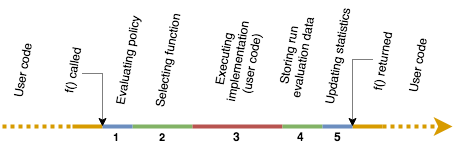
\includegraphics[width=100mm]{./img/run_schema.png}}}
	\caption{Process of combined function invocation.}
	\label{fig:run_schema}
\end{figure}

The policies are a suitable tool to limit the potential damage of the selection process to the system. For this, it is necessary to observe and to store various times connected with the selection and execution. Figure \ref{fig:run_schema} shows the whole process with policy being evaluated with the \textbf{SelectNew} result, split into individual parts. Upon every invocation, the following is tracked:

\begin{itemize}
	\item Selection and run history storage time (2 and 4)
	\item Function execution time (3)
	\item Total time spent on the \textbf{SelectNew} result (2, 3 and 4)
	\item Total time spent on the \textbf{GatherData} result (3 and 4, 2 is skipped in such a case)
\end{itemize}

Sums of these times are kept in every combined function. The policy can work with these numbers and analyze the changes that happen to them over time. In addition, the number of times each function was selected, the total number of times we received the \textbf{SelectNew} and \textbf{GatherData} result and the total number of times the combined function was invoked have to be tracked. 

In general the policy has the following data available to decide:

\begin{itemize}
	\item Total run count of the combined function
	\item Total number of times each function was selected
	\item Total number of times of gathering new data (\textbf{GatherData} result)
	\item Total time spent on function execution (after \textbf{SelectNew} result)
	\item Total time spent on selection and storage overhead (after \textbf{SelectNew} result)
	\item Total time spent on processing the \textbf{SelectNew} result
	\item Total time spent on processing the \textbf{GatherData} result
	\item Number of times the last selected function was selected in a row (the \textit{function streak})
\end{itemize}

\subsection{Implemented policies}

As mentioned earlier, policies are designed to be reusable as building-blocks. The immutable policy itself is the only holder of the state and change of state can be performed only by transitioning to a different policy. Its functionality and very simple decision-making process can be visualized using a transition diagram, which shows the policy itself as a dark (red) square with solid border, all the other policies as a lighter squares with either solid or dashed border (determines if the policy is an argument or not), and arrows as state transitions. The transitions might be conditional, in such a case, the condition splits the arrow into two. The transition can produce a result which is shown next to the transition arrow. If a result is produced, the policy makes a decision and next policy will be evaluated during the following invocation. If a result isn't produced, the policy just delegates the decision to the next policy which is evaluated immediately. The chain of evaluation stops when first result is produced.

The transition conditions use policy parameters, which are passed to a policy in the constructor, and the current statistical data explained in section \ref{subsec:statistical_data}. It can also use static fields and methods that it has access to. The parameters of the top-level (starting) policy are passed in by the user creating it, the parameters of the other policies in the chain are fixed when the policies are created, usually during the decision of the top-level policy, which typically builds the entire policy chain (that can be cyclic and lead back to it).

The transition diagrams and short descriptions of some policies will follow.

\subsubsection{Building blocks}

\begin{figure}[h!]
	\captionsetup{justification=centering,margin=0.5cm}
	\centerline{\mbox{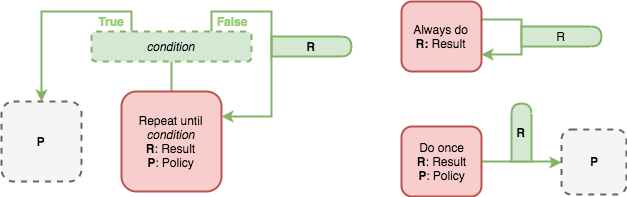
\includegraphics[width=130mm]{./img/helper_policies.png}}}
	\caption{Transition diagram of the basic building-block policies.}
	\label{fig:helper_policies}
\end{figure}

Figure \ref{fig:helper_policies} shows the main policies that serve as a building-blocks. The most important is the \textbf{Repeat until condition} policy, parametrized by a \textit{condition}, result \textit{R}, which it keeps producing until the \textit{condition} becomes true, and the policy \textit{P}, which it makes transition to at that moment. The \textbf{Always do} policy represents an infinite loop producing the same result \textit{R} every time, and the \textbf{Do once} policy produces the result \textit{R} once and immediately makes transition to the policy \textit{P}.

\begin{figure}[h!]
	\captionsetup{justification=centering,margin=0.5cm}
	\centerline{\mbox{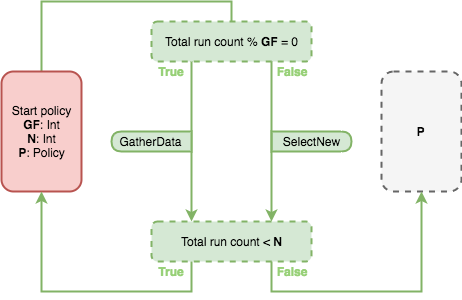
\includegraphics[width=80mm]{./img/start_policy.png}}}
	\caption{Transition diagram of the \textbf{Start policy}.}
	\label{fig:start_policy}
\end{figure}

Figure \ref{fig:start_policy} represents the \textbf{Start policy}, which accepts the gather frequency \textit{GF}, number of invocation times \textit{N} before moving to a next policy \textit{P}. It is a little more complicated and specialized version of the \textbf{Repeat until} policy - it keeps producing the \textbf{SelectNew} result, and every \textit{GF}-th invocation, it produces the \textbf{GatherData} result. It might be useful at the beginning, when it is necessary to gather data for all of the functions and perform some selections so that the following policies had statistical data to base their decision on.

\subsubsection{Stop selecting when decided}

\begin{figure}[h!]
	\captionsetup{justification=centering,margin=0.5cm}
	\centerline{\mbox{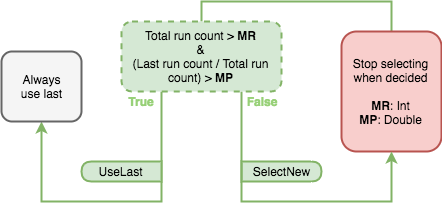
\includegraphics[width=90mm]{./img/stop_selecting_when_decided.png}}}
	\caption{Transition diagram of the \textbf{Stop selecting  when decided} policy.}
	\label{fig:stop_selecting_when_decided}
\end{figure}

In order to limit the overhead, it might be useful to completely stop selecting when we are sure that one of the functions gets selected a lot more often. The \textbf{Stop selecting when decided} policy shown in figure \ref{fig:stop_selecting_when_decided} keeps selecting new function until both the total number of invocations exceeds minimum run count \textit{MR} and the ratio of the number of times that the last selected function was selected and the total number of invocations exceeds the minimum percentage \textit{MP}. After that, it will keep using the last function forever. 

The advantage of falling back to the infinite \textbf{Always use last} policy is its basically zero overhead - no condition is evaluated in the decision process. So this policy is useful for the fast functions where keeping low overhead for the long-term is critical. It cannot, however, undo a wrong decision, reflect a change in conditions, or anything else.

\subsubsection{Pause selection after streak}

\begin{figure}[h!]
	\captionsetup{justification=centering,margin=0.5cm}
	\centerline{\mbox{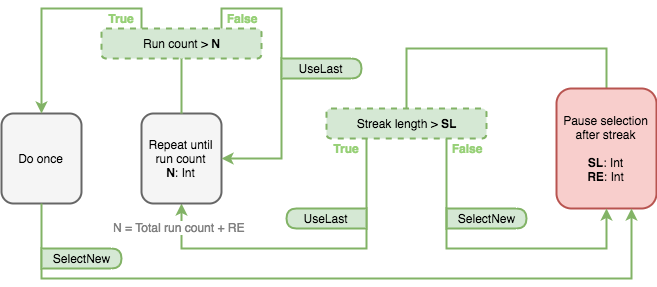
\includegraphics[width=110mm]{./img/pause_selection_after_streak.png}}}
	\caption{Transition diagram of the \textbf{Pause selection after streak} policy.}
	\label{fig:pause_selection_after_streak}
\end{figure}

To lower the number of selections, an approach based on the streak lengths can be used as well. It is implemented by the \textbf{Pause selection after streak} policy in figure \ref{fig:pause_selection_after_streak}. Its functionality is defined by the \textit{SL} (streak length) and \textit{RE} (retry every) arguments. Whenever one function is selected \textit{SL} times in a row, the selection process stops and the \textbf{UseLast} result is being produced. Once every \textit{RE} times, a new selection attempt is done, looping back to the original policy. If the same function is selected once again, the streak gets longer by one and the selection process stops again. If, however, a different function is selected this time, the streak becomes zero and we start selecting again.

The described behavior is the preferred way of limiting the selection overhead. By setting the streak length to a reasonable number (e.g. between 10 and 100, based on the data, situation, etc.), we can assure that if one function is significantly better than the others, it will be used without the need to select it. The retry that happens every once in a while makes sure that eventual wrong decision will be detected and will reset the system back to the beginning.

\subsubsection{Limited overhead, gather time and selection time}

\begin{figure}[h!]
	\captionsetup{justification=centering,margin=0.5cm}
	\centerline{\mbox{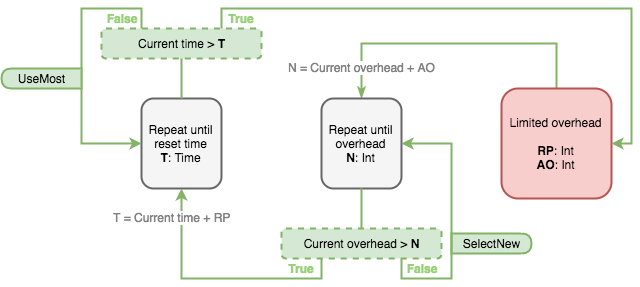
\includegraphics[width=110mm]{./img/limited_overhead.png}}}
	\caption{Transition diagram of the \textbf{Limited overhead} policy.}
	\label{fig:limited_overhead}
\end{figure}

Policies can be used to limit the framework involvement per a real-time period, so that the selection overhead or the time spent on gathering data does not damage the system more than a specified limit. The \textbf{Limited overhead} policy in figure \ref{fig:limited_overhead} limits only the selection overhead time to \textit{AO} (allowed overhead) every \textit{RP} (reset period). After depleting the allowed time, it cannot select anymore and keeps using the most selected function until the end of the period.

\begin{figure}[h!]
	\captionsetup{justification=centering,margin=0.5cm}
	\centerline{\mbox{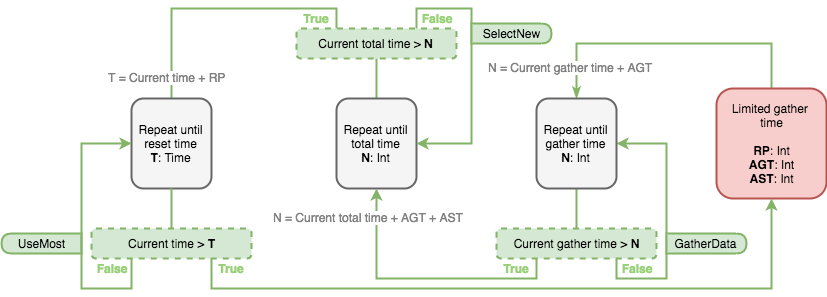
\includegraphics[width=110mm]{./img/limited_gather_time.png}}}
	\caption{Transition diagram of the \textbf{Limited gather time} policy.}
	\label{fig:limited_gather_time}
\end{figure}

In exactly the same way, the time spent on executing the function for the result \textbf{GatherData} and the whole process of selection and execution for the \textbf{SelectNew} result can be limited. The figure \ref{fig:limited_gather_time} demonstrates the \textbf{Limited gather time} policy, which keeps producing \textbf{GatherData} until total gather time reaches \textit{AGT} (allowed gather time), after that, it continues with the \textbf{SelectNew} result until total selection time reaches \textit{AST} (allowed selection time). A loop producing \textbf{UseMost} follows, for the rest of the real-time period specified by \textit{RP} (reset period).

This policy gives us control over the time spent on selecting results in real-time. If we get a lot of requests at the same time, receive a large batch of data to process or for any reason need to momentarily increase the throughput of the system, the time or overhead limits get depleted very quickly and the \textbf{UseMost} fallback result means reasonably good performance with a minimum overhead.

\subsection{Policy builder}

As we could see from the policy examples, most of them were built only using the \textbf{Repeat until} or \textbf{Do once} blocks in a loop. This process of combining these generic blocks into sequences can be automatized and hidden behind a simple DSL (see \ref{sec:dsls}) called \textit{policy builder} that would allow the user to express his customized way to decide about the function run.

Figure \ref{fig:policy_builder_chart} shows the syntax diagram of \textit{policy builder}.

\begin{figure}[h!]
	\captionsetup{justification=centering,margin=0.5cm}
	\centerline{\mbox{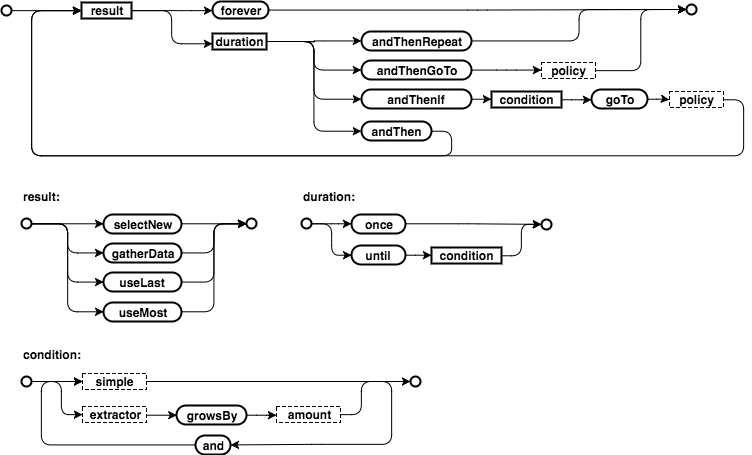
\includegraphics[width=140mm]{./img/policy_builder_chart.png}}}
	\caption{Syntax diagram of the \textit{policy builder} DSL.}
	\label{fig:policy_builder_chart}
\end{figure}

The policy built with \textit{policy builder} has always one main loop. Its definition starts with the first result that it emits: \textit{selectNew}, \textit{gatherData}, \textit{useMost} or \textit{useLast}. A result is always followed by a duration specifier, and another result. When we specify the sequence of results and their durations, we can end it by either closing the main loop (using \textit{andThenRepeat}), by transitioning to an external policy (using \textit{andThenGoTo}, leads to a policy out of the loop), or by using \textit{forever} as a duration for the last result, which limits the loop just this one result. In addition, it is possible to put a conditional transition to a policy out of the loop anywhere in between two results (using \textit{andThenIf}).

The conditions can be either simple functions accepting statistical data and returning a boolean value, or a \textit{growsBy} condition with a value extractor\footnote{A function that extracts a value of some type from the statistical data. Default implementations are provided for the basic fields.} and an amount. A simple condition is evaluated only once against current statistical data. In case of the \textit{growsBy} condition, the extractor is executed once at the beginning of the policy loop and its result is stored, and the condition evaluation consist of executing it and comparing current result to the stored one.

An example of a simple policy described using the \textit{policy builder} follows. It produces \textbf{GatherData} 50 times, then \textbf{SelectNew} 50 times, and then either loops forever on \textbf{UseLast}, if the streak is larger than 20, or repeats the whole process otherwise.

\lstset{style=Scala}
\begin{lstlisting}
val conditional: Policy = (
  gatherData until (totalRunCount growsBy 50)
  andThen selectNew until (totalRunCount growsBy 100)
  andThenIf ((stats: StatisticDataProvider) => stats.getStreakLength >= 20) goTo (useLast forever)
  andThenRepeat)
\end{lstlisting}

\subsection{Policies and groups}

One of the techniques for improving the selection process is grouping the history records using some input features, as described in \ref{subsec:grouping}. We will extend the grouping to function statistics and to the current policy. It means that the combined function needs to hold the policy and the statistical data for every group, and perform transitions and statistics updates separately.

The main advantage is the possibility to take faster decisions in some groups, using for example the \textit{Pause selection after streak} policy. When a function is significantly faster than the others for some category of inputs, the streak will build up fast within the group and the invocation for future inputs from such a group will require no selection and will be very quick, yielding correct results.

\subsection{Possible improvements}
\label{subsec:policy_improvements}

The policies were designed as a concept that is completely independent from the actual selection strategies and history analysis. One of the improvements that would require closer tying would be to allow the policies to choose the selection strategy, or to influence it somehow, by limiting it to a subset of data, etc. 

Another improvement that might seem useful is to let the policies analyze the whole history data. This would, however, mean a lot of additional overhead time when evaluating the policy, which is not desirable.
With a different approach, we could achieve the same thing by giving selection strategies a state that could involve their decision. The state would be managed by the combined function and it could even be the same state that is used by the policies. 

Next, a factor of combined certainty of all the selections of a specific function could be included in the statistical data. This factor could be aggregated from the selection results of the strategies that would support it (in the statistical test based strategies, it could be a p-value, strength of the test, or similar) and would serve as a decision factor for more complex policies.

%TODO - when do I need more data?

\chapter{Framework implementation}
\label{chap:implementation}

The API, as described in chapter \ref{chapter:api}, and the decision making logic from chapter \ref{chap:deciding} was implemented into the ScalaAdaptive framework, a simple library that can be added to any Scala project and allows the programmer to utilize the adaptive decision making in his application.

In this chapter, we will go through the implementation of the framework, its basic architecture and the possibilities to extend it. We will also mention some decisions that had to be made during the implementation.

\section{Goals of implementation}

The main concerns upon implementing the framework were the following:

\begin{itemize}
	\item To separate the API from the selection logic
	\item To keep the framework strongly typed and use static type checking even in the internal parts of the code
	\item To make the framework as extensible as possible
	\item To keep the framework overhead as low as possible
	\item To keep the code well-organized, to minimize code duplication
\end{itemize}

\subsubsection{Development approach}

The main development approach was based on using the Scala language features to make the code simpler, easier to maintain and less error-prone. We tried to benefit from the functional approach whenever possible, while still keeping the high-level design object oriented. It leads to having the data and functionality separated in different classes. Inheritance is used only for implementing traits (except for some special cases, like the API function objects). All of the functionality-providing classes are used via corresponding traits, and thus communicating only through a simple and limited interface, which allows replacing them very easily. These trait-based building blocks are put together using composition and delegation patterns.

\subsubsection{Error handling}

The framework is designed so that the number of exceptions handled in the code was minimized. The ScalaAdaptive itself does not raise almost any exceptions in case of errors\footnote{The only exception being custom identifier validation in the function combination.}, and catches most of the exceptions from the libraries within to replace them with a None return value.

This approach is known from the functional programming and takes advantage of monadic operations over the \textit{Option monad}\footnote{In Haskell and other languages known as Maybe monad.}. The return values can be mapped over using the \textit{bind} operator, which allows smooth function chaining and the error propagation through the chain. More details can be found in the talk \cite{noauthor_railway_nodate}.

\section{Architecture overview}
\label{sec:architecture_overview}

This section will provide brief overview of the entire framework architecture and related decisions. More detailed description at the level of individual classes can be found in the documentation (see  \hyperref[attach:scaladoc]{attachments}).
%TODO: Documentation reference

\subsection{API architecture}
\label{subsec:api_architecture}

As briefly described in section \ref{subsec:api_implementation}, the public API of the framework is represented by a set of traits \inlinecode{AdaptiveFunction0}, ..., \inlinecode{AdaptiveFunction5}, which expose all the user accessible methods. Because only some of the methods depend on the number of input arguments, the part of the API that can be generalized was extracted into a common trait \inlinecode{AdaptiveFunctionCommon}, which is parametrized by the function type that extends it. 

\begin{figure}[h!]
	\captionsetup{justification=centering,margin=0.5cm}
	\centerline{\mbox{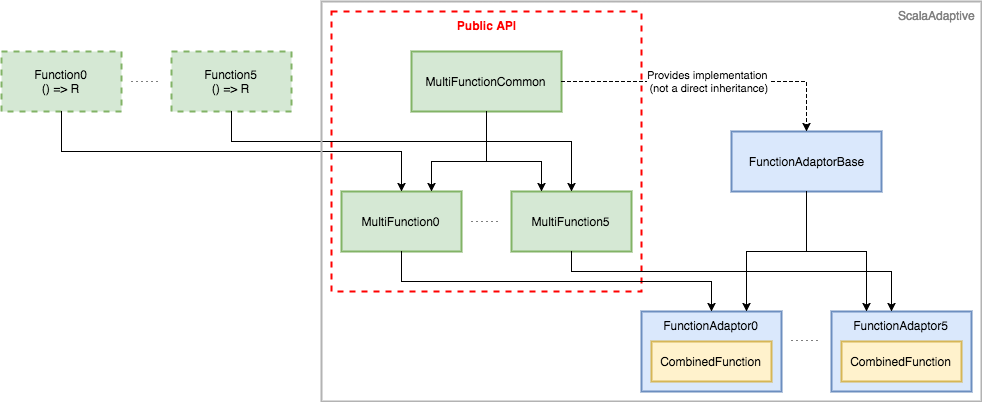
\includegraphics[width=140mm]{./img/inheritance_function_adaptors.png}}}
	\caption{Diagram showing the inheritance chain of MultifFunctionN and related classes.}
	\label{fig:inheritance_function_adaptors}
\end{figure}

The \inlinecode{AdaptiveFunctionN} traits are implemented by \inlinecode{FunctionAdaptorN} classes that are directly inaccessible to the user, which allows us to modify or extend their internal API without changing the public API, thus maintaining backwards compatibility. The methods that can be implemented independently on the number of input arguments are extracted into an abstract class \inlinecode{FunctionAdaptorBase} that the other adaptors inherit from.

It would be quite impractical to manipulate with N different classes that represent the combined functions inside the internal parts of the framework. Therefore, the actual class holding the functions, \inlinecode{CombinedFunction}, is wrapped inside each one of the \inlinecode{FunctionAdaptorN} and is parametrized by the tuple type consisting of all the N arguments of the original function, and by the return type. All the functions are converted into functions of type \inlinecode{(TArgType) => TRetType} in the following way:

\lstset{style=Scala}
\begin{lstlisting}
val tupleFunction = (tupleArg) => function(tupleArg._1, ..., tupleArg._n)
\end{lstlisting}
	
The whole inner part of our framework works only with \inlinecode{CombinedFunction} types and therefore with functions of type \inlinecode{(TArgType) => TRetType}. Individual function adaptor classes perform the composition of the arguments into the tuple version before propagating the call further whenever a method depending on the argument number is invoked.

The figure \ref{fig:inheritance_function_adaptors} shows this inheritance and composition scheme.

The user of the framework will generate the instances using implicit conversion methods defined on an \inlinecode{Implicits} singleton, a part of the API that is described in \ref{subsec:api_implementation}. The actual conversions where the \inlinecode{FunctionAdaptorN} and the \inlinecode{CombinedFunction} instances get created will be wrapped inside another singleton object, \inlinecode{Conversions}, and the delegating calls will be done using a macro due to reasons explained later.

\subsection{Internal architecture}
\label{subsec:internal_architecture}

The simplified internal architecture can be seen in the figure \ref{fig:internal_architecture}. It shows the core chain that is executed when a combined function, represented as a \inlinecode{AdaptiveFunctionN} to the user, but internally stored as a \inlinecode{CombinedFunction} instance, is called.

\begin{figure}[h!]
	\captionsetup{justification=centering,margin=0.5cm}
	\centerline{\mbox{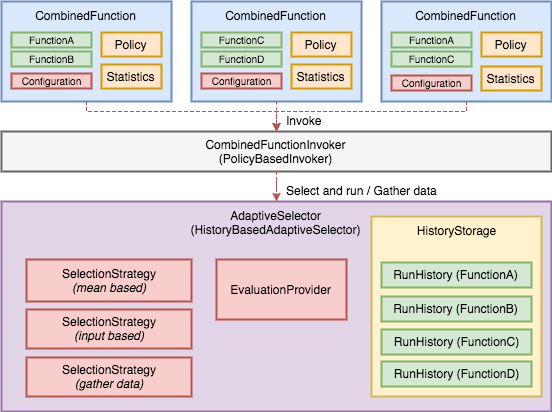
\includegraphics[width=140mm]{./img/internal_architecture.png}}}
	\caption{Diagram showing the internal architecture of the ScalaAdaptive framework.}
	\label{fig:internal_architecture}
\end{figure}


As we can see, there are two principal logic units participating in the process:

\begin{enumerate}
	\item \textbf{\inlinecode{CombinedFunctionInvoker}} \\
	Supposed to make a quick decision based on the \textit{policy} of the combined function. It should either directly invoke one of the functions, or delegate the call to the \inlinecode{AdaptiveSelector}, and update the statistics of the combined function afterwards. It works only with the data directly stored in the \inlinecode{CombinedFunction} instance, it does not have any state or shared storage.
	\item \textbf{\inlinecode{AdaptiveSelector}} \\
	The key component of the framework, it receives a set of functions and an input, and it should decide which one of them to run and to execute it, evaluate the function run and return the result. The default implementation works with an abstract history storage (\inlinecode{HistoryStorage}), three selection strategies (\inlinecode{SelectionStrategy}) and an evaluation mechanism (\inlinecode{EvaluationProvider}). It also offers an operation of invoking the function with least data directly.
\end{enumerate}

\section{Implementation options}

A few questions regarding the implementation arise from the basic architecture showed in section \ref{sec:architecture_overview}. We will provide a brief analysis before explaining the implementation details any further.

\subsection{History storage location}
\label{subsec:storing}

\inlinecode{HistoryStorage} is supposed to gather and store history data for all functions that are invoked using a combined function. The question is, where to save the data and how accessible to make it. We propose three variants.

\subsubsection{Local}

First option is to make the storage part of the \inlinecode{CombinedFunction} itself. In this case, the history data would, just like the statistics, be unique for every instance of the class, i.e. for every \inlinecode{AdaptiveFunctionN} created by the user. This has two consequences:

\begin{itemize}
	\item A function will have separate histories for every use in a combined function
	\item Every new instance of a combined function will have an entirely new history for all the functions
\end{itemize}

The second consequence might lead to some unexpected behavior - for example, if we create a combined function inside of a method call as described in section \ref{subsubsec:method_from_combined_func} and call it just once, it will have a clear history every time and will be useless:

\lstset{style=Scala}
\begin{lstlisting}
def processData(data: List[Int]): Int = 
  (impl1 _ or impl2 withStorage Storage.Local)(data)
\end{lstlisting}

Some use cases for this configuration exist, e.g. if we have a class that holds some immutable data and we keep executing some computations on the data, then a combined function defined as a field on this class with local storage will adapt specifically to the data of the class and does not need input based strategies.

\subsubsection{Global}

Another option is to store all the measured data globally, in a static area of the memory accessible from all contexts. This will allow to collect run data for functions faster and share them across all the combined functions, which usually leads to more informed and more precise decisions. This is usually the preferred approach for some business logic or utility methods in long-running services. A unique identifier has to be used to match the function history record with the actual function in the \inlinecode{CombinedFunction} class. The selection of the identifier will be discussed later.

\subsubsection{Persistent}

The biggest problem of the discussed storage locations is that the run history data are available only during a single run of the application. Whenever the application restarts, it will have to collect the data again. This might not be a problem for some long running services or daemons, but it is not very convenient for some tools or client applications with shorter lifecycle.

A solution to the problem is storing the data in a persistent storage, (e.g. HDD). We can do it in three different ways:

\begin{enumerate}
	\item Immediately persist each run history record
	\item Persist all of the records when the application terminates
	\item Buffer the history records and persist them in batches
\end{enumerate}

The first option seems like the best one, but it would lead to a series of I/O operations upon every invocation of a combined function. The added overhead of this solution could be dramatic. The second option, on the other hand, has no runtime overhead at all, but it requires a possibility to detect an application termination from our framework. JVM does not guarantee finalizers being called and relying on notifications from the user would complicate the API and be problematic in general. 

There is a mechanism in JVM called \textit{shutdown hooks} that allow the user to perform a custom action on shutdown (for more details see \cite{noauthor_jvmshuthooks_nodate}). It will, however, not be called when the application crashes. Additionally, it might be unexpected from a library to perform actions on shutdown and the delay that caused by persisting a lot of run data on a slow HDD (or even a network drive) could lead to the application being terminated immediately in some automatized environments.
Therefore, the third option was selected, as it leads to the runs being regularly saved and the I/O overhead is lower.

The persistence relies on the unique function identifier as well. There are additional problems connected to persisting the run history, namely:
\begin{itemize}
	\item Running multiple instances of the application at once (collisions on the persisted data file)
	\item Changes in the application code (outdated run data, changed identifiers, etc.)
	\item Having to deal with larger amounts of history data
\end{itemize}

\subsection{History storage function identifiers}
\label{subsec:function_identifiers}

As described in section \ref{subsec:storing}, we need some sort of identifier of the function to be able to store the run history data in a global or persistent storage. It does not make sense to use the references to the function objects, as new closure instances are created every time a lambda expression (or an eta-expanded method) is assigned, which would lead to having new history for each new instance, a behavior equivalent to local storage discussed in \ref{subsec:storing}.

%TODO: Reference an example?

This leaves us with three basic identifier options.

\subsubsection{Type name}

As explained in \ref{subsec:functiontypes}, functions in Scala are instances that extend the \inlinecode{FunctionN} trait. The default implementations are anonymous closure classes that are compiled from lambda expressions. Two different functions originate in two different lambda expressions and thus have two different type names, the ones that were generated and assigned by the compiler. The fully qualified type name can be used as the identifier of a function

Using the type names as unique identifiers is safe and straightforward. A small disadvantage is that they are not very readable, the compiler uses the name of the type that contained the lambda expression followed by sequential number. 

There is also a subtle danger connected - if we try to combine two different function that originated from the same lambda expression (the difference might be determined by the closure arguments), they will have the same identifier, thus sharing the same history, which is usually not desirable.

The next problem is that in case of persisting the run history, the closure classes might get renamed automatically upon recompiling. The compiler usually assigns the closure names sequentially, so this could happen by just inserting another lambda expression into the enclosing class code before the current one. Run history data might even get mixed up as the newly added lambda expression could have the former name of the original closure (by taking its position in the sequence).

Last but not least, If the \inlinecode{FunctionN} trait has a different than default implementation, the type name identification might fail - the trait can be implemented by a single class wrapping other values. In this case, all functions implemented by that class would share the run history.

\subsubsection{Method name}
\label{subsec:methodnameident}


The expected most common usage pattern of the framework is the one where the functions used with the \inlinecode{or} method are \textit{eta-expanded} methods (see \ref{subsubsec:apimethods}). There is a problem connected with methods when using the type name identifiers - every time a method gets eta-expanded, a new lambda expression with new type name is generated. In the following case, the \inlinecode{method1} would not have the same identifier in the two combined functions:

\lstset{style=Scala}
\begin{lstlisting}
val fun1 = method1 _ or method2
val fun2 = method1 _ or method3
\end{lstlisting}



It would be handy to use the method name as an identifier in such a case, which would lead to better readability and allow the same method used in different combined functions to have just one run history.

The problem is that at runtime, the implicit type conversion method or the \inlinecode{or} method will always get the already \textit{eta-expanded} function object with a compiled \inlinecode{apply} method holding the actual method call inside. The names have to be extracted at compile time, using the def macros (see \ref{sec:defmacros}). At the moment of the implicit conversion from \inlinecode{FunctionN} to \inlinecode{AdaptiveFunctionN} (as described in \ref{subsec:api_implementation}), the AST\footnote{Abstract syntax tree.} of the \inlinecode{FunctionN} expression can be examined - if it's a lambda expression containing one method call, the method name can be extracted. The exact process how to do so will be presented in a separate section.

\subsubsection{Custom identifier}
\label{subsubsec:custom_identifier}

In order to handle the specific cases where type name and method name identifiers do not distinguish correctly between different functions, there is also a possibility of choosing a custom, arbitrary identifier. This has to be triggered specifically by the user in the API and should be used in the cases where:

\begin{enumerate}
	\item User knows that the automatically assigned identifiers will not be sufficient
	\item User wants to replace default type identifier with custom identifier because of readability
\end{enumerate}

\section{Extracting method name from eta-expansion AST}
\label{sec:extracting_method_name}


In the description of the API in section \ref{subsec:api_implementation}, we introduced an implicit method that will perform the conversion from \inlinecode{FunctionN} to \inlinecode{AdaptiveFunctionN}. In order to extract the method name from potential uses of eta-expanded methods in this conversion, we will have to implement it in the following way:

\begin{enumerate}
	\item Replace the implicit conversion method by a def macro (see \ref{sec:defmacros}) and extract the conversion logic into a different, non-implicit method that allows explicitly setting the function identifier (in our case, the \inlinecode{Conversions} singleton object methods \inlinecode{toAdaptor()})
	\item Inside the implicit macro, analyze the AST and try to locate the eta-expansion method call
	\item If the method call is successfully found:
	\begin{enumerate}
		\item Generate the identifier expression as a \inlinecode{getTypeName} call on the target of the method call, concatenated with the method name
		\item Generate the conversion code with explicitly specified identifier expression
	\end{enumerate}
	\item Otherwise generate the conversion code with implicit identifier	
\end{enumerate}

The conversion is done using the \inlinecode{toAdaptor()} method with two overloads:
\begin{itemize}
	\item Accepting only the function - implicit identifier is used (type name of the closure)
	\item Accepting the function and a custom identifier - the identifier provided is used
\end{itemize}

\subsection{Eta-expansion AST format}

First step in the macro implementation has to be parsing the input AST and detecting patterns that are generated from eta-expansions by the compiler. Using the \inlinecode{printAst()} macro mentioned in \ref{subsec:buildingast}, the following facts were discovered:

\begin{itemize}
	\item The eta-expansion is already replaced by the equivalent code in AST, so it cannot be detected directly.
	\item The result of eta-expansion is a lambda expression (referred to as function literal in the AST).
\lstset{style=Dump}
\begin{lstlisting}
Function(...)
\end{lstlisting}
	\item The lambda expression is always wrapped in a block, being its return value.
	
\lstset{style=Dump}
\begin{lstlisting}
Block(
  List(...), 
  Function(...))
\end{lstlisting}	
	
	\item If the target of the invocation is either a constant or \textit{this}, it is captured in the lambda expression closure (i.e., the constant or \textit{this} is referenced directly from the function body).
	
	\item If the target of the invocation is a variable or a result of a more complicated expression, it is extracted to the enclosing block, its result is stored in a variable local to the block and then captured in the lambda expression closure. The following example shows how the target, originally an expression \inlinecode{this.getInstance()} on a \inlinecode{Class} class, was extracted into the block body.
	
\lstset{style=Dump}
\begin{lstlisting}
Block(
  List(
    ValDef(
      Modifiers(SYNTHETIC), 
      TermName("eta$0$1"), 
      TypeTree(), 
      Apply(
        Select(
          This(
            TypeName("Class")), 
          TermName("getInstance")), 
        List()))), 
  Function(...))
\end{lstlisting}

	\item The function node contains argument definition and the expression itself, which is a single application (method call).

\lstset{style=Dump}
\begin{lstlisting}
Function(
  List(
    ValDef(
      Modifiers(PARAM | SYNTHETIC), 
      TermName("arg"), 
      TypeTree(), 
      EmptyTree)), 
  Apply(...))
\end{lstlisting}
\end{itemize}

This has a few consequences for our case. First, we will look for functions with a body consisting from one method call. Secondly, we need to generate our conversion code (along with the method retrieval) into the block return value, because we need to be able to access the actual invocation targets that might exist only in the block (as the original expression was extracted and replaced by a local variable). The target and the method name will always be in the single Apply node representing the function body.

\subsection{Retrieving the target from the method call}

Now we need to go through the method call subtree and locate the invocation target. If the method does not accept any type arguments, the structure is quite simple:

\lstset{style=Dump}
\begin{lstlisting}
Apply(
  Select(
    ...invocation target expression..., 
    TermName("methodName")), 
  List(...function arguments...))
\end{lstlisting}

Where the \textit{invocation target expression} can have multiple forms based on the original expression, and can depend on the enclosing block variables. It is not, however, important for us, as we can work with the expression as whole. The function arguments are not needed either.

If the method is generic, the type arguments need to be applied in order to convert it to a function (which can't be generic). In this case, the tree gets a little more complicated:

\lstset{style=Dump}
\begin{lstlisting}
Apply(
  TypeApply(
    Select(
      ...invocation target expression..., 
      TermName("genericMethod")), 
    List(...type arguments...))), 
  List(...function arguments...))
\end{lstlisting}

The method call is wrapped in a TypeApply node before being invoked using the Apply node. The TypeApply node can be ignored in our case.

And the most complicated case we are going to analyze is when the method has some implicit arguments as well:

\lstset{style=Dump}
\begin{lstlisting}
Apply(
  Apply(
    TypeApply(
      Select(
        ...invocation target expression...,
        TermName("genericMethodImplicit")), 
      List(...type arguments...)), 
    List(...function arguments...)), 
  List(...implicit arguments...))
\end{lstlisting}

One more Apply node is added to the topmost level - the implicit arguments are applied after applying the actual function arguments. Their definition contains another nested block and lambda expression, but again, it is not important for our case. We just need to extract the invocation target and the method name, which can be both found in the Select node in one of the previous cases.

Note that there are situations where the eta-expansion might lead to more complicated trees, for example when used on methods with multiple argument lists. These are, however, cases which we are not going to support with the extraction.

\subsection{Generating the conversion}
\label{subsec:generate_conversion}

Supposing we have the invocation target expression and the method name, we need to create the identifier string expression that will be used in the manual \inlinecode{toAdaptor} invocation.

In order to extract the fully qualified name of the method call target, we need to generate the following expression:

\lstset{style=Scala}
\begin{lstlisting}
invocationTarget.getClass.getTypeName + ".methodName"
\end{lstlisting}

The AST representing this expression has to be wrapped in a construction application of \inlinecode{MethodNameIdentifier} class (it is a case class with automatically generated \inlinecode{apply()} method) to get the resulting identifier.

In all the cases, the \inlinecode{toAdaptor} method has to be generated to replace the macro function. The function literal from the original AST has to be passed in as the first argument, and optionally, the second argument containing the method name identifier can be provided if the extraction of the method name was successful.

The original tree in a simplified form can be seen in figure \ref{fig:original_eta_ast}.

\begin{figure}[h!]
	\captionsetup{justification=centering,margin=0.5cm}
	\centerline{
		\begin{forest}
			[Block
			[Statements
			[ValDef]
			]
			[Function]
			]
		\end{forest}
	}
	\caption{The original simplified eta-expansion AST.}
	\label{fig:original_eta_ast}
\end{figure}

We need to transform the block, keeping the definition in the statement part, but wrapping the \inlinecode{Function} into the \inlinecode{toAdapter} call, as shown in figure \ref{fig:transformed_eta_ast}.
	
\begin{figure}[h!]
	\captionsetup{justification=centering,margin=0.5cm}
	\centerline{
		\begin{forest}
			[Block
			[Statements
			[ValDef]
			]
			[Apply
			[toAdaptor]
			[ArgumentList
			[Function]
			[ExtractedIdentifierExpression]
			]
			]
			]
		\end{forest}
	}
	\caption{The simplfied eta-expansion AST after manually adding toAdaptor call.}
	\label{fig:transformed_eta_ast}
\end{figure}

\subsection{Extracting method overloads}

The approach that was described so far has one small issue - it does not recognize function overloads, so all the overloads share the same identifier.

 It would not be difficult to extract the actual number of arguments that the method is being invoked with and include it in the identifier. As for extracting their types, the situation gets a little complicated - the function literal is generated without argument type specification, the TypeTree is empty:

\lstset{style=Dump}
\begin{lstlisting}
ValDef(
  Modifiers(PARAM | SYNTHETIC), 
  TermName("i"), 
  TypeTree(), 
  EmptyTree)
\end{lstlisting}

This is a valid AST in Scala and can be generated in a lot of situations, for example:

\lstset{style=Scala}
\begin{lstlisting}
val function: (Int) => Int = { i => math.abs(i) + 1 }
\end{lstlisting}

In this case, the lambda expression does not have the type of its arguments specified either, because the compiler will infer it from the context in which the expression is used, in this case, from the type specifier of the variable it is being assigned to.

The compiler is able to infer the data type from the usage of the argument as well\footnote{The code snippet is correctly compiled by the Scala compiler, although some IDEs (namely IntelliJ IDEA 2016.3.4) are not able to infer the type and mark the code as incorrect.}:
\lstset{style=Scala}
\begin{lstlisting}
def method(i: Int): Int = ???
val function = { i => method(i) }
\end{lstlisting}

Note that the eta-expansion is guided by the same rules, so whenever expanding a method without overloads, the compiler infers the types by itself:
\lstset{style=Scala}
\begin{lstlisting}
def method(i: Int): Int = ???
val function = method
\end{lstlisting}

Upon expansion of a method with overloads, the resulting function type has to be provided either explicitly, or as an expected type in an expression (e.g. inside a method argument). The inference flow goes in the other direction in such a case:
\lstset{style=Scala}
\begin{lstlisting}
def method(i: Int): Int = ???
def method(s: String): Int = ???
val function: (String) => Int = method
def useFunction(fun: (Int) => Int): Unit = ???
useFunction(method)
\end{lstlisting}

As a consequence, at the time of syntax analysis, the types are not inferred yet and there is no way for us to find out which method overload is being called.

The method overloads therefore have to share the same identifier. If it leads to a problem, a type name or a custom identifier can be used in such a case.

\subsection{The conversion demonstration}

As a practical demonstration of the process described in this section, we are going to show the compile-time conversions that are done on a method identifier that is being \textit{eta-expanded} and converted into a \inlinecode{AdaptiveFunctionN}. Let's consider the following code:

\lstset{style=Scala}
\begin{lstlisting}
val combined = target.method _ or function
\end{lstlisting}

We will follow the conversions that the compiler and our macro perform on the \inlinecode{target.method \_} expression\footnote{The actual changes are performed on the AST level, we will show them in corresponding Scala code for simplicity.}:

\begin{enumerate}
	\item The explicit \textit{eta-expansion} is performed:
	\lstset{style=Scala}
	\begin{lstlisting}
{ () => target.method() }
	\end{lstlisting}
	\item The implicit conversion is applied:
		\lstset{style=Scala}
	\begin{lstlisting}
Implicits.toAdaptiveFunction0({ () => target.method() })
		\end{lstlisting}
		\item The macro \inlinecode{toAdaptiveFunction0} is executed and expanded:
		\lstset{style=Scala}
		\begin{lstlisting}
Conversions.toAdaptor({ () => target.method() }, MethodNameIdentifier(this.getClass.getName + ".method"))
		\end{lstlisting}
\end{enumerate}

The final state shows the code that will be present in our compiled program and will be executed.

\subsection{Macros in the combining method}

In the section \ref{subsubsec:apimethods}, we explained why the \inlinecode{or} method has to accept an argument of \inlinecode{FunctionN} type instead of \inlinecode{AdaptiveFunctionN}. This does not seem to cause any trouble as we can manually convert \inlinecode{FunctionN} into the \inlinecode{FunctionAdaptorN} inside the method body. With the macro expansion, however, we run into problems. Image we do it the following way:
\lstset{style=Scala}
\begin{lstlisting}
def or(fun: (T1) => R) = orAdaptiveFunction(Implicits.toAdaptiveFunction1(fun))
\end{lstlisting}

The  \inlinecode{toAdaptiveFunction1} method is a macro - it gets executed at compile time, and it receives the argument AST as its input. In this case, an AST that consists of the \inlinecode{fun} identifier. We have no way to find out, where this function will be called from and with which arguments, so in order to extract the method name, we need to convert the entire \inlinecode{or} function to a macro which will generate the conversion code in the same manner as described in section \ref{subsec:generate_conversion}, and then wrap it in the internal \inlinecode{orAdaptiveFunction} code.

This does not require any extra AST manipulations, only one method call generation. It does, however, mean a complication for us, as the macros cannot be called virtually. The macro definition therefore has to be a part of the \inlinecode{AdaptiveFunctionN} API trait, breaking somehow the encapsulation of the implementation. Fortunately, it does not perform any actions by itself, only replaces the \inlinecode{or} call with a conversion and an \inlinecode{orAdaptiveFunction} call, which is, again, a virtual method defined on the trait without implementation and therefore encapsulated.


\section{Module implementation}
\label{sec:module_impl}

All the modules mentioned in \ref{subsec:internal_architecture} are abstract traits with replaceable implementations, that are put together using composition. The API classes have to be able to access the composed and active implementations at the moment of invocation. For this reason, a singleton Scala object \inlinecode{AdaptiveInternal} was introduced and holds the following composed modules:

\begin{itemize}
	\item \inlinecode{AdaptiveSelector} with global storage
	\item \inlinecode{AdaptiveSelector} with persistent storage
	\item \inlinecode{CombinedFunctionInvoker}
\end{itemize}

We will briefly introduce the implementations of these modules and the parts that they are composed from.

\subsubsection{CombinedFunction}

The \inlinecode{CombinedFunction} is the main data class representing a function with multiple implementations in ScalaAdaptive. It is basically a data holder class, the important functionality was separated to be easily replaceable. It gets created and modified when a user of the framework manipulates with the \inlinecode{AdaptiveFunctionN} API type. Part of its attributes are immutable, representing the configuration and default setup of the function, and part of its attributes are mutable, holding its state in the invocation process.

It contains the following immutable data:

\begin{itemize}
	\item Set of functions that it is combined from (wrapped into the tuple form, see \ref{subsec:api_architecture})
	\begin{itemize}
		\item	Each function holds up to two identifiers - one based on the closure type name, the other being either a method name or a custom name, depending on the creation process (see \ref{subsec:function_identifiers})
	\end{itemize}
	\item \textit{Descriptor function} (wrapped into the tuple form), see \ref{sec:input_based_strategies}
	\item \textit{Group selector} function (wrapped into the tuple form), see \ref{subsubsec:group_selection}
	\item Function configuration defined by the user, will be described later in more detail
\end{itemize}

And the following state representing data:

\begin{itemize}
	\item Function statistics (separately for each group, see \ref{subsec:statistical_data})
	\item Current \textit{policy} (separately for each group, see \ref{sec:policies})
	\item Analytics data - full list of all the selections and their results
\end{itemize}

In case of the local storage setup, the instance also has to contain its own \inlinecode{AdaptiveSelector} that holds the local \inlinecode{HistoryStorage}.

\subsubsection{CombinedFunctionInvoker}

It has access to the state of the \inlinecode{CombinedFunction} and its basic implementation does the following:

\begin{itemize}
	\item Evaluate the current \textit{policy} with the statistics of the combined function
	\item According to the result either invoke directly the function which is accessible through the statistics (the last one and the most selected one) in case of \inlinecode{UseLast} or \inlinecode{UseMost} results , or pass the decision onto the \inlinecode{AdaptiveSelector} in case of \inlinecode{SelectNew} or \inlinecode{GatherData} results
	\item Update the function statistics
\end{itemize}

The \inlinecode{AdaptiveSelector} is accessed either through the \inlinecode{CombinedFunction} itself for the local storage setup, or using the singleton object \inlinecode{AdaptiveInternal} in case of global or persistent setup.

\subsubsection{AdaptiveSelector}

A module which is supposed to select one of given options to run, and to evaluate the run. It is parametrized with \inlinecode{TMeasurement} type, which represents the data measured from the function run. By default, a \inlinecode{Long} type for run time measured is used. It supports two basic operations - \textit{selectAndRun} and \textit{gatherData}, which correspond to the \textit{policy} results. Both of these operations have also an option with delayed measurement (see \ref{subsec:delayed_measuring}).

The implementation \inlinecode{HistoryBasedAdaptiveSelector} contains the general chain described in \ref{sec:selection_and_invocation_process}. It uses a \inlinecode{HistoryStorage} to store and retrieve the run data of individual functions. In addition, it holds three \inlinecode{SelectionStrategy} instances, one for gathering new data, one for the input based selection, and one for the mean based selection. One of these three instances is used to select the function to run, which is then executed using an \inlinecode{EvaluationProvider}. The measurement retrieved is added to the history and the result is returned, along with a performance benchmark including execution and overhead times (independent on the actual measurement, always based on wall-clock times) for the function statistics update. Figure \ref{fig:history_based_selector} shows the entire process.

In case of the operations with delayed measurement, the function run is not evaluated, an \inlinecode{InvocationToken} is generated instead. The token holds a callback to the \inlinecode{AdaptiveSelector} and whenever used to invoke some function, it will use the \inlinecode{EvaluationProvider} to evaluate the run and store the data to the corresponding history record.

Note that the \inlinecode{SelectionStrategy} for gathering new data should select a function for which data are needed the most at the moment instead of optimizing the performance.

\begin{figure}[h!]
	\captionsetup{justification=centering,margin=0.5cm}
	\centerline{\mbox{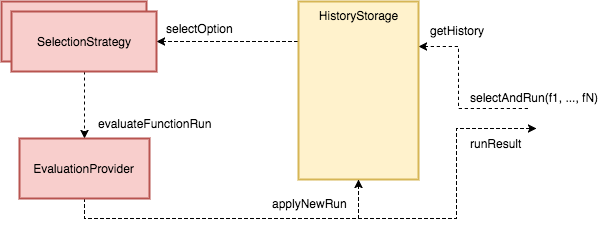
\includegraphics[width=100mm]{./img/history_based_selector.png}}}
	\caption{Diagram showing the HistoryBasedAdaptiveSelector execution path.}
	\label{fig:history_based_selector}
\end{figure}

\subsubsection{HistoryStorage}

A type with a map-like interface based on the concepts from section \ref{subsec:storing_evaluation_data} - it is supposed to hold the historical measurement vectors represented by \inlinecode{RunHistory} instances for each combination of function and group. A key composed of the function identifier and the group identifier is used to access the histories.

There are two implementations in the framework:

\begin{itemize}
	\item\inlinecode{MapHistoryStorage} - stores the histories in memory
	\item\inlinecode{PersistentHistoryStorage} - a wrapping storage that delegates the calls to an internal \inlinecode{HistoryStorage}, and, in addition, it serializes every new run using a \inlinecode{HistorySerializer} and if asked for a history that is not present in the underlying storage, it tries to deserialize it using the same class
\end{itemize}

The \inlinecode{HistorySerializer} has two basic implementations, one for direct serialization, and one for buffered serialization. The data are stored into a file, one per function, and the format, root directory and file name pattern are fully customizable. There is no list of these history containing files anywhere - when trying to deserialize a function, a file with corresponding name is checked for existence. This means that the individual function histories are deserialized one by one, at the moment of the first invocation of a combined function that contains them, which might cause a delay in the first execution.

\subsubsection{RunHistory}

\inlinecode{RunHistory} represents the vector of historical measurement results and other details about a function run. The interface is designed to support immutable solution - the appending methods always return an instance of the same type, which might or might not be the same object depending on the implementation. The interface provides some basic operations on the history, allows iteration over the data and appending new data (always at the end). 

Apart from that, it also has some methods to directly provide precomputed data for some of the selection strategies in order to support caching. These supporting methods can always be computed using the data available, and if the implementation of \inlinecode{RunHistory} does not support the caching or precomputation, there are \textit{mixin} traits\footnote{Traits that contain functionality that can be included in a class.} with default implementations available.

The provided implementations of \inlinecode{RunHistory} can be chained using the \textit{Decorator} pattern to modify the behavior. The basic implementations are the following:
\begin{itemize}
	\item \inlinecode{FullRunHistory} - stores all runs in an \inlinecode{ArrayBuffer}, is mutable
	\item \inlinecode{ImmutableFullRunHistory} - stores all runs in an immutable \inlinecode{List}, is a little slower in general
\end{itemize}

These instances can be wrapped in the following decorator classes:
\begin{itemize}
	\item \inlinecode{LimitedRunHistory} - limits the maximum number of stored items, whenever it reaches maximum, it throws the older half of all the records away
	\item \inlinecode{CachedStatisticsRunHistory} - stores the statistical data about the run items, speeds up the t-test strategy (see \ref{subsec:t_test_multiple})
	\item \inlinecode{CachedGroupedRunHistory} - stores average evaluation data for each \textit{run selector}, speeds up the local regression strategy (see \ref{subsec:local_regression})
	\item \inlinecode{CachedRegressionRunHistory} - stores the linear regression model built upon all the run items, speeds up the linear regression strategy (see \ref{subsec:simple_linear_regression})
\end{itemize}

The \inlinecode{LimitedRunHistory} wrapper should always be used, as it can prevent unexpected out-of-memory exceptions in the program run, as the base run history implementations have no size limits.

\subsubsection{SelectionStrategy}
\label{subsubsec:selection_strategy_impl}

Very simple trait that represents the selection strategies described in detail in sections \ref{sec:input_based_strategies} and \ref{sec:mean_based_strategies}. The implementations should be stateless and should work only with the \inlinecode{RunHistory} records that it receives (in order not to mix together decisions about two separate history storage locations). The strategy implementations often have a customizable fallback strategy that is used in cases where the current strategy is not able to make a decision, as described in section \ref{subsec:solving_decision_failures}.

The strategies are parametrized by the \inlinecode{TMeasurement} type of the function run evaluation. All of the implemented strategies work with function run time represented either directly by \inlinecode{Long} or by a type viewable as \inlinecode{Numeric}.

The mean based strategies consist of the following classes:
\begin{itemize}
	\item \inlinecode{TTestSelectionStrategy} - implements the t-test strategy described in section \ref{subsec:t_test_multiple}, uses \cite{noauthor_apachemath_nodate} to compute the p-value.
	\item \inlinecode{UTestSelectionStrategy} - implements the u-test strategy described in section \ref{subsec:u_test}, uses \cite{noauthor_apachemath_nodate} to compute the test statistics.
\end{itemize}

The implemented input based strategies are:
\begin{itemize}
	\item \inlinecode{RegressionSelectionStrategy} - implements the linear regression strategy as described in section \ref{subsec:simple_linear_regression}, uses the \cite{noauthor_apachemath_nodate} to compute the regression

	\item \inlinecode{LoessInterpolationSelectionStrategy} - implements the local regression strategy from section \ref{subsec:local_regression}, uses the \cite{noauthor_apachemath_nodate} for the interpolation
\end{itemize}

In addition, some complementary supporting were added:
\begin{itemize}
	\item \inlinecode{WindowBoundSelectionStrategy} - a wrapper strategy that limits the history records to a flexible window as described in sections \ref{subsec:window_bound_regression} and \ref{subsec:window_bound_t_test}
\item \inlinecode{LowRunAwareSelectionStrategy} - if any of the functions has less than a specified number of history records, uses one strategy, otherwise, uses a different strategy
\item \inlinecode{LeastDataSelectionStrategy} - uses the function with least historical runs
\end{itemize}

The common pattern is to use the \inlinecode{LowRunAwareSelectionStrategy} as the topmost strategy in the composition to postpone the decision process until some data are ed, the \inlinecode{LeastDataSelectionStrategy} as the fallback strategy, and to have one of the actual input based or mean based strategies in the middle, optionally wrapped in the window-bound class. The \inlinecode{LeastDataSelectionStrategy} is also recommended to be used as the strategy for the \textit{gather data} operation of \inlinecode{AdaptiveSelector}.

\subsubsection{EvaluationProvider}

With a goal of potentially supporting larger variety of possible function evaluation data, the selected function is always executed using an implementation of \inlinecode{EvaluationProvider}, which is supposed to run the function and to evaluate it, and return both the result of the function and the evaluation data in the form of \inlinecode{TMeasurement}. The default implementation simply measures the wall-clock time of the function run.

\section{User interaction and customization}

The basic behavior of the combined functions can be changed in two ways:
\begin{itemize}
	\item Each combined function can have the most basic features configured individually
	\item The whole framework can be re-configured and customized
\end{itemize}

\subsection{Combined function setup}
\label{subsec:function_setup}

As the basic API designed in chapter \ref{chapter:api}, i.e. the \inlinecode{or} method used to create new combined functions, does not allow directly setting the function behavior, a simple configuration API has to be added. In compliance with the DSL-like \inlinecode{or} chaining, the configuration was made possible via special methods on the \inlinecode{AdaptiveFunctionN} type that allow chaining as well\footnote{In the \textit{builder}-style pattern, by returning the same type.} and are also meant to be used like operators. The combined function definition including the configuration can be very fluent and natural:

\lstset{style=Scala}
\begin{lstlisting}
val sort = standardSort _ or selectionSort by (_.size) selectUsing Selection.InputBased storeUsing Storage.Global
\end{lstlisting}

\subsubsection{Input descriptor and group selector}

The most important part of the configuration API are the \inlinecode{by} and \inlinecode{groupBy} methods. The first allow the user to specify the \textit{descriptor function}, i.e., function describing how to extract an \textit{input descriptor} from the input (see \ref{subsec:input_in_selection}). A function of type \inlinecode{(T1, ..., TN) => Long} is used for that, where \inlinecode{T1, ..., TN} are the arguments of the \inlinecode{AdaptiveFunctionN}. 

The second method expects a \textit{group selector}, which assigns the input to a certain group (see \ref{subsubsec:group_selection}). It should receive a function of type \inlinecode{(T1, ..., TN) => Group}.

\subsubsection{Function configuration}

Additional behavior can be modified for the combined function. The choice is based mostly on selecting which one of multiple implementation options should be used with given function. In the \inlinecode{AdaptiveInternal} singleton, we hold two implementations of \inlinecode{AdaptiveSelector}, one with persistent history storage, the other without. Each of these two implementations then includes two instances of  \inlinecode{SelectionStrategy}, one for input based and one for mean based selection.

The function configuration methods and possible values are the following:

\begin{itemize}
	\item \inlinecode{storeUsing} - represents the history storage options as described in section \ref{subsec:storing}
	\begin{itemize}
		\item \inlinecode{Global} - uses the shared \inlinecode{AdaptiveSelector} without persistent storage
		\item \inlinecode{Persistent} - uses the shared \inlinecode{AdaptiveSelector} with persistent storage
		\item \inlinecode{Local} - creates a new instance of \inlinecode{AdaptiveSelector} locally in the function object
	\end{itemize}
\item \inlinecode{selectUsing}
\begin{itemize}
	\item \inlinecode{InputBased} - uses the input based strategy in \inlinecode{AdaptiveSelector}
	\item \inlinecode{MeanBased} - uses the mean based strategy in \inlinecode{AdaptiveSelector}
\end{itemize}
\item \inlinecode{limitedTo} - allows to specify the maximum age of the history records to be used in the selection process, as described in \ref{subsec:limiting_record_age}
\item \inlinecode{asClosures} - represents the history storage identifier choice as described in section \ref{subsec:function_identifiers}
\begin{itemize}
	\item \textit{true} - always uses closure type names as the function identifiers
	\item \textit{false} - uses either method names or custom names as the function identifiers if available
\end{itemize}
\item \inlinecode{withPolicy} - allows to specify the starting policy for the function, as described in \ref{sec:policies}
\end{itemize}

The user is expected to specify this configuration with most of the combined functions. The default values are determined by the framework configuration, except for the selection strategy choice, which is defaulted to input based if the \textit{descriptor function} is provided for the combined function and to mean based otherwise.

\subsection{Logging, analytics and control access}

There are two basic mechanisms for the user of the framework to observe its functionality - logging and analytics.

\subsubsection{Logging}

Logging is performed by multiple parts that are involved in the selection process. An instance of the simple \inlinecode{Logger} trait held in the \inlinecode{AdaptiveInternals} and passed around to other modules is used for that purpose. The provided implementation of loggers are \inlinecode{ConsoleLogger}, \inlinecode{FileLogger} and \inlinecode{EmptyLogger}, where the last one does not actually save the logs anywhere, and is used by default to limit the overhead.

Replacing \inlinecode{EmptyLogger} with one of the other types will lead to detailed output describing each invocation of every combined function, which can be used to trace eventual problems with the framework behavior.

\subsubsection{Analytics and control access}
\label{subsubsec:analytics}

To provide a more systematic and technical access of the framework behavior, a simple set of methods was made accessible on the \inlinecode{AdaptiveFunctionN} type by extending the \inlinecode{AdaptiveFunctionControl} and \inlinecode{AdaptiveFunctionAnalytics} traits:

\begin{itemize}
	\item \inlinecode{train} - trains the combined function on a given set of inputs (by executing all of the functions on each of the inputs and storing the results)
	\item \inlinecode{flushHistory} - flushes the entire run history of given function (in the corresponding history storage)
	\item \inlinecode{setPolicy} - sets the current \textit{policy} of the function to a custom one
	\item \inlinecode{resetPolicy} - sets the current \textit{policy} of the function to the starting one
	\item \inlinecode{getAnalyticsData} - retrieves analytics data regarding the function history
\end{itemize}

The analytics data represent a way of monitoring the decisions of the selection process for each combined function. It contains a complete set of records of previous runs, each one holding the identifier of the selected function, the \textit{input descriptor}, run time and the overhead time spent on the selection. The data can either be analyzed directly in the application by processing these records, or can be easily serialized into a CSV file.

Note that the analytics data collection is relies on the \inlinecode{AnalyticsCollector} trait. Again, we provide two implementations, \inlinecode{BasicAnalyticsCollector} that collects all the data mentioned, and \inlinecode{EmptyAnalyticsCollector}, that does not collect anything. The empty variant is default in order to minimize the overhead of the framework. In case the user has a need of the analytics data from his application, he can enable the collection by replacing the collector.

\subsection{Framework configuration}
\label{subsec:framework_config}

In section \ref{sec:module_impl}, we mentioned a variety of building blocks that the main parts of the framework are composed of, and the possibility to use multiple implementation to change the behavior of the entire system. This is the more advanced part of the configuration and it requires manipulation with the actual implementations.

As explained earlier, all the shared and commonly accessible functionality is held inside the singleton object \inlinecode{AdaptiveInternal}. This object can be initialized using an \inlinecode{initialize()} method on a publicly accessible singleton \inlinecode{Adaptive}. The static description of the composition of the implementations that is followed in this process is provided by a \inlinecode{Configuration} trait. This can be though of as a composition root of the whole system - it has to provide factory functions for all the building blocks used. In addition, it has an abstract type member \inlinecode{TMeasurement} for the evaluation data. 

%TODO: Add ref to http://docs.scala-lang.org/tutorials/tour/abstract-types.html

The implementation of the \inlinecode{Configuration} trait has to provide a specific \inlinecode{TMeasurement} type and the factory methods that rely on the type. Note that the \inlinecode{AdaptiveSelector} trait and its methods do not depend on the \inlinecode{TMeasurement}, only its implementation does, so the type of the evaluation data does not leak outside of the composition root. As a result, the actual type can be changed at runtime by simply replacing the \inlinecode{AdaptiveSelector} instance.

The \inlinecode{Configuration} can be created by the user himself, using either a combination of provided implementation or his custom implementations. Alternatively, one of the predefined \inlinecode{Configuration} traits with some basic settings already implemented can be utilized:

\begin{itemize}
	\item \inlinecode{BaseConfiguration} - provides basic configuration of some of the types that do not depend on the \inlinecode{TMeasurement}
	\item \inlinecode{BaseLongConfiguration} - sets the \inlinecode{TMeasurement} type to \inlinecode{Long} and adds basic configuration of some of the types that depend on it
\end{itemize}

These traits have to be extended to define the unimplemented values.

\subsubsection{Configuration blocks}
 To simplify the configuration process when working with existing implementations and to hide the initialization details from the user, a concept called \textit{configuration blocks} was introduced. 
 
 \textit{Configuration blocks} are traits that provide implementation for just one (or a few) functions from the \inlinecode{Configuration} trait, setting up part of the framework in given way. The user of the framework can then define the configuration by creating an anonymous class extending the base configuration along with desired \textit{configuration blocks}. Thanks to the fluent and simple syntax of Scala, this concept is very expressive and easy to use. The compile-time check will automatically alert the user if the combination of block does not cover some required method.
 
 In addition, some blocks can be parametrized. The parameters are always protected read-only attributes of the block trait that usually have default implementation (i.e. value), but can be overridden. It fits easily into the anonymous class usage pattern, as the new parameter values for all the blocks can simply be stated in the body of the class. Blocks can share a parameter by inheriting it from the same base trait - in such a case, it is impossible to set different values for different blocks.
 
 The whole configuration can look the following way:

\lstset{style=Scala}
\begin{lstlisting}
val config = new BaseLongConfiguration
  with DefaultHistoryPath
  with RunTimeMeasurement
  with WindowBoundRegressionInputBasedStrategy
  with UTestMeanBasedStrategy
  with CachedRegressionAndStatisticsStorage
  with FileLogging {
  override val maximumNumberOfRecords = 20000
  override val alpha = 0.25
  override val logFilePath = "./adaptive/log.txt"
}

Adaptive.initialize(config)
\end{lstlisting}

List of all the configuration blocks available along with their parameters can be found in appendix REF.

%TODO: ADD THE APPENDIX / ATTACHMENT REFERENCE!

\subsubsection{Default configuration}

A special class for the default configuration was created, which is used to initialize the ScalaAdaptive framework at the beginning of the application run and which specifies the implementations that are used if the user does not provide his configuration.

Based on the results observer in section \ref{sec:strategy_comparison}, we decided to include the t-test selection strategy with cached statistics as the mean based strategy, and the window-bound linear regression as the input based strategy.

The default configuration can be extended with any of the configuration blocks as well:

\lstset{style=Scala}
\begin{lstlisting}
val config = new DefaultConfiguration with ConsoleLogging
\end{lstlisting}

\subsection{Extending the framework}

The framework can be simply extended without actually modifying it by creating custom implementations of some of the traits that are used by the invocation and selection process, and by supplying it to the \inlinecode{Adaptive} initialization using a custom configuration, as described in \ref{subsec:framework_config}.

An overview of the areas that are the simplest and most useful to extend will follow.

\subsubsection{Selection strategies}

A new selection strategy can be created by extending the \inlinecode{SelectionStrategy} trait and by providing the implementation as either input based or mean based selection strategy. The trait itself is technically a single function corresponding to the algorithm mentioned in \ref{subsec:selecting_function}, which is given a sequence of function run histories and an input descriptor and is supposed to return the key (function identifier and group identifier) of the function with best expected performance:

\lstset{style=Scala}
\begin{lstlisting}
def selectOption(records: Seq[RunHistory[TMeasurement]], 
  inputDescriptor: Option[Long]): HistoryKey
\end{lstlisting}

The strategy will most likely have to work with either a specific \inlinecode{TMeasurement} data type, or at least put a constraint on it (by using the \textit{viewability} mechanism, see section \ref{subsec:implicit_args}).

\subsubsection{History storages}

If we wanted to change the way in which the history data are stored, e.g. by filtering some of the results, performing some aggregations to save space, etc., we would need to implement one or both of the following traits - the \inlinecode{RunHistory} trait, that represents the sequence of results for one group and function, and the \inlinecode{HistoryStorage} trait, that manages the \inlinecode{RunHistory} instances for different groups and functions.

\subsubsection{Evaluation data}

We can change the \inlinecode{TMeasurement} data type and make the framework perform the adaptations according to a different (or more complex) evaluation results. In such a case, we need to implement the \inlinecode{EvaluationProvider} trait, and then add our custom selection strategies that select based on the new evaluation type.

\section{Framework distribution and usage}

The framework is distributed in a form of JAR package containing all its compiled classes, which can be found in the \hyperref[attach:cd]{attachments}. The simplest way to set up ScalaAdaptive in any Scala project is to use the SBT (see \cite{noauthor_sbt_nodate}). The \inlinecode{scalaadaptive.jar} file needs to be placed into the \inlinecode{lib} folder in the project root. SBT will automatically locate the content of the archive and add the required classes in the \textit{classpath}.

Now, in any of the Scala source files in the corresponding project, the following line can be added:
\lstset{style=Scala}
\begin{lstlisting}
import scalaadaptive.api.Implicits._
\end{lstlisting}

From now on, the original Scala function types have been enhanced with the ScalaAdaptive methods, including the most important \inlinecode{or} method, that allows creating functions with adaptive execution. The usage is described in detail in section \ref{sec:api_usage}, a brief description of other options can be found in section \ref{subsec:function_setup}. A complete documentation is included in the \hyperref[attach:scaladoc]{attachments}.

The framework can be configured using the following call:
\lstset{style=Scala}
\begin{lstlisting}
scalaadaptive.api.Adaptive.initialize(configuration)
\end{lstlisting}

The \inlinecode{configuration} object functionality is described in \ref{subsec:framework_config} along with simple examples. The whole list of blocks that can be used in the configuration process is also available in the \hyperref[attach:config_blocks]{attachments}.
\chapter{Evaluation}

An~example citation: \cite{Andel07}


\section{Artificial algorithm}
\section{Sorting algorithm}
\section{... General algorithm - predicting the big O notation ...}
\section{SQL query selection}
\section{Spark}
\subsection{What is Spark}

\subsection{Spark APIs}

Spark currently supports three different APIs that can be used to construct Spark queries.

\subsubsection{RDD}

RDD (Resilient Distributed Dataset) was the first API introduced and is based on chaining higher order functions like \inlinecode{map()}, \inlinecode{filter()}, etc. RDDs contain custom JVM objects, Spark isn't aware of its structure. The query is typed and constructed using lambda expressions that work with these objects. It gets executed when a function that doesn't produce new RDD is called, e.g. \inlinecode{collect()} or \inlinecode{count()}. 

Example of a simple query:
\lstset{style=Scala}
\begin{lstlisting}
rdd.filter(_.id > 5000).count
\end{lstlisting}

Upon execution, the Spark worker engine works with the RDDs as a whole (partitions it, collects the results, etc.), but the operations on its members (filtering, transformation, grouping) are carried out by actually executing the lambdas. This approach is very simple and allows the user to write queries over custom data types without any limitation. The downside is that the Spark execution engine doesn't know what is going on within the lambdas, can't optimize the execution plan based on the query, and, when moving the parts of RDDs between the nodes, the objects have to be serialized and deserialized again.

\subsubsection{Dataframes}

Dataframes API 

\subsubsection{Datasets}
\subsection{RDD query selection}
\subsection{RDD or Datasets selection}
\subsection{Usage}
\subsection{Environment}
\section{Server selection}

\section{JSON parsing libraries}
\label{subsec:jsonparsing}

\section{Problems with the practical use of the framework}

\subsection{Selection overhead}
\subsection{Maintainability}

One of the main problems that such a framework is facing in a real-life software system is an engineering problem. The code of today's systems has to be kept working and maintained for several years, sometimes decades. During this period, bugs appear in the system, business requirements change and consequently, it is necessary to perform changes and adaptations in function code.

Maintaining multiple implementations of the same functionality at once brings a lot of issues. The developers have to know exactly how all the implementations work and whenever it's necessary to modify the behavior, be able to perform changes in all of them to achieve the same result. Described process itself is very demanding and has a significant time impact on the development. 

What's more, subtle differences in behavior of the implementations could be unintentionally introduced. These differences might not have visible effects immediately and may appear after several other modifications. At that moment, it will be extremely difficult to locate the problem, because the misbehavior caused by it won't be deterministic thanks to the nature of the selection algorithm.

Using non-deterministic decision tools in general lowers the maintainability of the system.

\subsection{Debugging}

Discovering and fixing bugs in a software system is a key part of its development and maintenance process. It is a very complex and time consuming activity, and its complexity grows considerably for the bugs that have non-deterministic occurrences. Whenever there is a bug in one of the implementations used with the framework, it is inherently non-deterministic, as it has effect only when the specific implementation is selected.

\section{Other tests...?}

\section{Usage from Java}

\section{Usage from Kotlin}

%TODO: Usage from Java & Kotlin

\section{Implementation in other languages}

The framework is implemented in Scala and can be used by any JVM-based languages, even though often without the comfort that provides Scala with its implicits and eta-expansion.

The same functionality, however, could be used on other platform than JVM as well. The framework itself isn't complicated to reproduce and its runtime back-end is transferable to basically any platform. There would be minor complications with immutability of the data structures and expressiveness of Scala in some cases, but nothing show stopping.

The key part of the framework that would cause problems upon reimplementation is the API, which relies heavily on Scala's DSL features (see \ref{sec:dsls}). It requires the following features from the language:

\begin{itemize}
	\item Implicit type conversions
	\item Functions as first-class values
	\item Eta-expansion of methods
	\item Infix operator syntax for methods
	\item Macros to parse and modify the AST upon compilation
\end{itemize}

With a subset of the features in the language, a limited API can be designed. Let's have a look at some language examples and what they offer.

\subsection{Kotlin}

\subsection{Java}

\subsection{C\#}

The C\# language has relatively advanced features and offers function types (\inlinecode{Func<TArg, TRetVal>}) that allow treating the functions as first class values. There is also a feature called \textit{Method groups}, which, in certain situations, lead to an implicit conversion of a method on an object to the corresponding function type - basically the same as eta-expansion.

%TODO: Add examples

The API in C\# could be based on method chaining and be quite similar to the one in Scala, although the method name extraction and the infix fluent-language syntax wouldn't be present.

\subsection{Python}
???

\subsection{C / C++}
\chapter{Related work}

A different approach for the same goal consists in manually selecting an implementation and guaranteeing its performance with unit tests. A special language, SPL (Stochastic Performance Logic), which allows to express assumptions about the performance of multiple functions, was introduced in \cite{bulej_capturing_2012}. The innovative concept is that it treats the performance as a random variable, not as a fixed value, so the conditions are evaluated with certain confidence. It was later used to examine the performance of JDOM framework in \cite{horky_performance_2013}, and became the base of performance unit testing frameworks for C\# (\cite{Trojanek:Thesis:2013}) and Java (\cite{Kotrc:Thesis:2015}).

The development of adaptive systems that can tweak their performance based on the environment is a widely studied topic as well. Systems that are capable of some form of \textit{auto-tunning}, i.e., self reconfiguration based on an analysis of the execution environment (OS, CPU, etc...), are often among the fastest in its category - an example might be \cite{frigo_fftw:_1998},  which is considered to be the fastest non-commercial FFT\footnote{Fast Fourier transform} algorithm in the world. The adaptation in this case is done by recompiling the application code (\cite{frigo_fast_1999}).

An idea of a universal adaptive framework that would not require manual analysis of the environment and work only with observations from actual execution is presented in \cite{bulej_performance_2012}. It describes a system that has generally the same goal as our work - increase performance awareness by designing the systems adaptively. It is focused on large component-based applications where the performance of certain components is tracked. Multiple use-case scenarios are presented, e.g. verifying component contract, observing trends, or selecting between multiple interchangeable components based on performance. The SPL is used to make the decisions, i.e., the components are guarded by conditions expressed in the language.

The article does not solve the issue of predicting run time on a certain input based on the performance on other inputs. In a case when the component does not have a run data for the input, it is executed with generated data of given size. The presented concept is also based on the interconnection between the adaptive framework and the system components. ScalaAdaptive provides a partial implementation of a similar system, more narrowly focused, which puts higher emphasis on the simplicity and efficiency of performing the single task of selecting faster implementation. In addition, it provides an API that allows easily using the adaptivity in any existing system with no need of architectural changes.

The problem of predicting function (or application in general) run time based on the input is a separate problem examined in many different ways. In \cite{wegbreit_mechanical_1975}, a statical analysis of LISP programs is performed in order to derive actual complexity. A runtime analysis approach was taken in \cite{goldsmith_measuring_2007}, where basic blocks in the program called \textit{locations} are identified and their performance is measured for a certain input described by a set of \textit{features}. The performance is represented by an execution count in order to keep the measurement deterministic and platform or environment independent. A powerlaw regression is then built to find relations between \textit{feature} values and \textit{locations}. The resulting model can be used to formulate predictions.

Relatively precise predictions of an actual execution can be achieved using the Mantis framework \cite{chun_mantis:_2010}, which is based on instrumenting the code and automatically identifying its \textit{features} (loops, branches, variable values...). The features are evaluated (branch counts, loop counts) at runtime and the machine learning process is used to select the ones that are important for the overall performance. A regression model is then constructed using the data. One of the possible models is described in \cite{huang_predicting_2010}.

Authors of \cite{smith_predicting_1998} obtain the predictions in two steps - first, they use greedy or genetic algorithm to find similar inputs (jobs, workloads) in the historical run measurement, and then, they generate the prediction using either simple mean or a linear regression, both with corresponding confidence interval. The basic approach taken here is quite similar to the ScalaAdaptive, even though neither this, nor the other works referenced in this chapter deal with the problem of real-time prediction upon invocation, where the main concern is minimizing the overhead.

\chapter*{Conclusion}
\addcontentsline{toc}{chapter}{Conclusion}

In this thesis, we designed and implemented a framework that allows a completely new style of performance-aware development by composing functions from interchangeable implementations. An API that allows fluent integration with almost no effort from the developer was introduced. Various statistical methods to identify the most appropriate implementation for given input based on historical performance observation were examined, implemented and compared.

The testing that was carried out identified potential use-cases for this style of development. Among the more suitable ones were in general longer running functions, where the run time fluctuations were not as significant and where the selection overhead was negligible. We achieved better overall run times of adaptive functions in artificial scenarios with input adaptation, either in case of an algorithmic problem (matrix multiplication), or in case of selection between two of the most used libraries.

In addition, we demonstrated a potential of environment adaptation on the Spark distributed data processing framework, where various configurations and query types achieved better results in different environments. The Spark itself has a big potential in the adaptivity, as it is being actively developed and many features have experimental character and are being iteratively optimized. On the other hand, the overhead caused by the invocation effectively prevents us from using the adaptation with quick and simple functions.

Among the main drawbacks of the solution is the fact that the user still has to identify the key feature of the input, which has to be one-dimensional (simple integer) in order to enable predictive selection. The prediction models are not perfect, especially in cases where the observed performances of all the functions are very similar. When we are, in addition, selecting from more than two functions, we might get stuck in a situation where the selection strategy cannot decide due to a pair of equally good functions and all of the functions are being used in a round-robin manner.

The majority of current problems and issues can be addressed in the future by extending the framework and adding new functionality. This can be done without actually modifying the framework code due to the modularity and run-time composition.

We believe that the biggest potential of this framework lies in its simplicity and possibility to be used in any kind of system without any structural changes. As we do not expect a common developer to implement one functionality multiple times and then combine it using our library, the main use-case in some larger project would most likely consist in combining multiple libraries, configuration, queries or other simply obtainable entities.

To see the actual benefit that this development approach can bring to a larger system, we would need to practically test it in such an application, i.e. a long running service, and track the performance changes. This kind of test would also expose other problems connected with either the framework, or the whole concept of adaptive development, that could not have been identified in the isolated artificial tests.

%%% Bibliography
%%% Bibliography (literature used as a source)
%%%
%%% We employ bibTeX to construct the bibliography. It processes
%%% citations in the text (e.g., the \cite{...} macro) and looks up
%%% relevant entries in the bibliography.bib file.
%%%
%%% The \bibliographystyle command selects, which style will be used
%%% for references from the text. The argument in curly brackets is
%%% the name of the corresponding style file (*.bst). Both styles
%%% mentioned in this template are included in LaTeX distributions.

%\bibliographystyle{plainnat}    %% Author (year)
\bibliographystyle{unsrt}     %% [number]

\renewcommand{\bibname}{Bibliography}

%%% Generate the bibliography. Beware that if you cited no works,
%%% the empty list will be omitted completely.

\bibliography{bibliography}

%%% If case you prefer to write the bibliography manually (without bibTeX),
%%% you can use the following. Please follow the ISO 690 standard and
%%% citation conventions of your field of research.

% \begin{thebibliography}{99}
%
% \bibitem{lamport94}
%   {\sc Lamport,} Leslie.
%   \emph{\LaTeX: A Document Preparation System}.
%   2nd edition.
%   Massachusetts: Addison Wesley, 1994.
%   ISBN 0-201-52983-1.
%
% \end{thebibliography}


%%% Figures used in the thesis (consider if this is needed)
\listoffigures

%%% Tables used in the thesis (consider if this is needed)
%%% In mathematical theses, it could be better to move the list of tables to the beginning of the thesis.
\listoftables

%%% Abbreviations used in the thesis, if any, including their explanation
%%% In mathematical theses, it could be better to move the list of abbreviations to the beginning of the thesis.
\chapwithtoc{List of Abbreviations}

\begin{itemize}
	\item \textbf{JVM} -- Java Virtual Machine, the target platform of Java, Scala and other languages
	\item \textbf{HTML} -- Hyper Text Markup Language
	\item \textbf{API} -- Application Programming Interface
	\item \textbf{REST} -- Representational State Transfer, a philosophy of web API
	\item \textbf{JSON} -- JavaScript Object Notation, a format for data exchange
	\item \textbf{XML} -- Extensible Markup Language, a format for data exchange
	\item \textbf{FFT} -- Fast Fourier Transform
	\item \textbf{JAR} -- Java Archive, a package format to distribute JVM based applications
	\item \textbf{SPL} -- Stochastic Performance Logic
	\item \textbf{OS} -- Operating System
	\item \textbf{CPU} -- Central Processing Unit
	\item \textbf{I/O} -- Input / Output
	\item \textbf{IoC} -- Inversion of Control, an application development pattern
	\item \textbf{AST} -- Abstract Syntax Tree, the result of syntax analysis of a code
	\item \textbf{DSL} -- Domain Specific Language
	\item \textbf{SBT} -- Scala Build Tools
	\item \textbf{RDD} -- Remote Distributed Dataset, a Spark API
\end{itemize}

%%% Attachments to the master thesis, if any. Each attachment must be
%%% referred to at least once from the text of the thesis. Attachments
%%% are numbered.
%%%
%%% The printed version should preferably contain attachments, which can be
%%% read (additional tables and charts, supplementary text, examples of
%%% program output, etc.). The electronic version is more suited for attachments
%%% which will likely be used in an electronic form rather than read (program
%%% source code, data files, interactive charts, etc.). Electronic attachments
%%% should be uploaded to SIS and optionally also included in the thesis on a~CD/DVD.
\chapwithtoc{Attachments}
\label{attachments}
\renewcommand{\thesection}{\Alph{section}}

\section{The enclosed disc contents}
\label{attach:cd}

A disc is enclosed 

\section{ScalaAdaptiveEvaluation project}
\label{attach:eval_project}

The ScalaAdaptive project contains only the framework, as it uses compile-time macros and therefore cannot be used from the same compilation unit. The ScalaAdaptiveEvaluation project contains all the source code that uses with the ScalaAdaptive framework. The important parts of the project are the following:

\begin{description}
	\item [evaluation] Package containing all the tests that were used to generate evaluation data. In each of the subpackages, there are Scala objects that have the \inlinecode{main} method and run the test. Each test contains a brief description about its inputs and output.
	\item [tutorials] Package containing a set of examples serving as simple introduction to the usage of the framework.
	\item [tests] Package containing mostly uncommented tests that were written and used in the process of development of the ScalaAdaptive framework.
\end{description}

\section{Scaladoc documentation}
\label{attach:scaladoc}

A detailed automatically generated documentation of all the classes in the ScalaAdaptive framework is enclosed on the disk. The 

\section{Complete list of configuration blocks}
\label{attach:config_blocks}

The following blocks can be used to configure ScalaAdaptive. If there is not a suitable block, a custom configuration implementation can be done.

\subsubsection{Analytics}
\begin{itemize}
	\item \inlinecode{AnalyticsCollection} - turns on the analytics data collection
	\item \inlinecode{NoAnalyticsCollection} - turns off the analytics data collection
\end{itemize}

\subsubsection{Logging}
\begin{itemize}
	\item \inlinecode{ConsoleLogging} - framework logs to the standard output
	\item \inlinecode{FileLogging} - framework logs to a specified file (\textit{logFilePath} argument)
	\item \inlinecode{NoLogging} - framework does not log
\end{itemize}

\subsubsection{Persistence}
\begin{itemize}
	\item \inlinecode{BufferedPersistence} - framework persists the run data in batches of \textit{serializationBufferSize} into a directory (\textit{rootHistoryPath} argument)
	\item \inlinecode{DirectPersistence} - framework persists the run data into a directory (\textit{rootHistoryPath} argument)
	\item \inlinecode{NoPersistence} - framework does not persist the data, global storage is used for persistent setup
\end{itemize}

\subsubsection{Selection strategies}
Sets the corresponding strategy as the main strategy of given type. Note that the \inlinecode{LowRunAwareStrategy} is always used as a wrapper with configurable \textit{lowRunLimit} argument. Some strategy blocks allow setting \textit{alpha} and \textit{averageWindowSize} arguments.
\begin{itemize}
	\item \inlinecode{LinearRegressionInputBasedStrategy}
	\item \inlinecode{LoessInterpolationInputBasedStrategy}
	\item \inlinecode{TTestMeanBasedStrategy}	
	\item \inlinecode{UTestMeanBasedStrategy}
	\item \inlinecode{WindowBoundRegressionInputBasedStrategy}
	\item \inlinecode{WindowBoundTTestInputBasedStrategy}
\end{itemize}

\subsubsection{History}
\begin{itemize}
	\item \inlinecode{CachedGroupHistory} - caches average run times for input descriptors
	\item \inlinecode{CachedRegressionHistory} - caches linear regression model
	\item \inlinecode{CachedStatisticsHistory} - caches statistics (used for T-test)
\end{itemize}

\openright
\end{document}
